\documentclass[twoside,english]{uiofysmaster}

\bibliography{references}
\usepackage{simplewick}
\usepackage{float}

% Adding nicer font to listings
\usepackage{ifxetex}
\ifxetex
  \usepackage{fontspec}
  \newfontfamily\listingsfontfamily[Scale=0.85]{Droid Sans Mono}
  \renewcommand{\listingsfont}{\listingsfontfamily}
\fi

\setlength{\parskip}{1em}

\author{Fredrik Wilhelm Holmen}
\title{A Study of Coupled-Cluster Methods for infinite matter}
\date{Autumn 2016}

\begin{document}
% set space around equations
\setlength{\belowdisplayskip}{12pt} \setlength{\belowdisplayshortskip}{12pt}
\setlength{\abovedisplayskip}{12pt} \setlength{\abovedisplayshortskip}{12pt}


\maketitle


\begin{abstract}
	In this thesis, we present the formalism of many-body methods,
        with an emphasis on the Coupled Cluster method with double
        excitations. The methods are tested on three physical systems,
        the finite size pairing model and two infinite homogenoeus
        systems, the electron gas in three dimensions and infinite
        nuclear matter. We have developed a software suite which can
        easily be extended to other physical systems, as well as to
        include more complicated correlations. The results have been
        benchmarked against existing literature. 
\end{abstract}

\begin{acknowledgements}
	The work I have done in this thesis could never been done without the help of Morten Hjorth-Jensen, my advisor. You have taught me everyting I have used in this thesis, through your many great courses and personal interactions. I want to thank you for the amazing work you have done for the group Computational Physics and for the way you inspire everyone you meet. The material I present in this thesis are built heavily upon the work of others. A special thank you to Audun Skau Hansen. My work is influenced by your great thesis. 

	I would like to thank Henrik Sveinsson for being a great inspiration and a good friend. You taught me the value of hard work and high ambitions. It was you who sparked my interest in physics at Oslo katedralskole when I followed your path in natural sciences. I would also like to thank Bj\o rnar Pettersen and Marit Ingebrigtsen, two of my teachers at Oslo katedralskole. 

	The last five years have been an amazing experience. I have learned way more than I thought was possible, I have met great people and been given opportunities by the institute to develop my skills as a tutor. Much of the positive experience is owed to the community at Lillefy, the home of Fysikkforeningen and Fysisk Fagutvalg, where I have emptied countless cups of coffee. Vetle Wegner Ingeberg, Henrik Limseth, Torgeir Mo, Sigve Smedsrud Harang, Anders Lauvland have been my best friends for the last five years. You have selflessly shared your knowledge, good humour and beers. 

	I am thankful for my time at Computational Physics, a splendid master group, filled with brilliant and caring people. You have created a relaxed atmosphere, where interesting discussions and competitive card games light up the day. A special thank you to Marte Julie Sætra, Jonas van den Brink, Sean Bruce Miller and Emilie Fj\o rner for sharing my office and giving me loads of help. 

	Thank you My Tien Diep for always keeping my motivation high and reducing my nerdy obsessions to a tolerable level.

\end{acknowledgements}


\tableofcontents


\begin{chapter}{Introduction}
	The aim of this thesis is to utilize many-body methods for
        computing the ground state energy for three different
        systems. The pairing model, the homogeneous electron gas and
        infinite nuclear matter. Well-performing many-body methods
        are very computationally costly, and a brute force
        implementation of configuration interaction theory, many-body perturbation
        theory and coupled-cluster theory is only a viable
        option for small systems. The thesis investigates how one can
        implement a more efficient solver for the coupled-cluster
         equations in order to gain a better  understanding of large systems.

	\begin{subsection}{Motivation}
		The pairing model is an interesting model to solve,
                not because of its direct representation of real
                matter, but because it lives in a small and finite
                Hilbert space. This allows us compute the exact ground
                state energy with full configuration interaction
                theory. The result is an important tool for comparing
                the performance of different solvers. Because it is a
                small and confined system, it is easy to calculate
                matrix elements, leading to an exact solution that
                lends itself for comparisons with methods like
                many-body perturbation theory and coupled-cluster
                theory. The system is therefore exceptionally good at
                benchmarking the implementation of many-body methods.

		Moving on to the homogeneous electron gas, we present
                an infinite system of electrons interacting with each
                other and a background charge. By only taking care of
                the electron-electron interaction, we generate a system
                that can be dealt with using common tools of many-body
                quantum mechanics. This is one of the first systems to
                be evaluated by many-body methods, and the literature
                on this topic contains many different benchmarks.


		The main goal of nuclear physics, is to understand the
                fundamental physics of the nucleus, its constituents
                and their interaction. We can generate experimental
                data on ground state energies, and by applying
                known many-body quantum mechanics, we hope to
                reproduce these results and gain larger insights into
                the forces and laws of motion which govern nuclear physics. 
                Studies of infinite matter and its equation of state have important consequences for 
dense objects like neutron stars or how a supernova evolves in its late stages.

	\end{subsection}

	\begin{subsection}{Goals for the Work}
		I have worked systematically to achieve the goals set up by the introduction to the thesis. The main goals of this thesis can be summarized in a few points: 
		\begin{itemize}
			\item A first goal for the thesis has been to
                          present the theory behind four many-body
                          methods. Starting with fundamental many-body
                          quantum mechanics and second quantization
                          before deriving the equations for
                          configuration interaction theory, Hartree-Fock
                          theory, Rayleigh-Schr\"{o}dinger
                          perturbation theory and coupled-cluster
                          theory.
			\item The second goal was to implement the Pairing model and the four solvers, coded in c++. The implementations could compute the ground state correlation energy to compare the efficiency of different solvers. The Pairing model could also serve as valuable benchmarking for the solvers.
			\item Next, I needed to present and implement the homogeneous electron gas system and the infinite nuclear matter system with neutrons. Only the coupled-cluster doubles equations would be used to compute correlation energies for these systems. 
			\item The original, brute force, coupled-cluster solver is too slow to compute correlation energies for large basis sets. I needed to look at how matrix-matrix multiplication and symmetries of the system could be exploited to reduce the computational costs. Presenting and implementing a much more advanced and efficient coupled-cluster doubles code has been the hardest and most time-consuming part of the thesis. 
      \item An important goal when developing the advanced coupled-cluster solver, was to make it as a good foundation for further expansions in the future. It should be object oriented and modular to allow for fast and easy expansions. It should also run in parallel. 
			\item Finally, the last goal has been to produce results for large basis sets for both the homogeneous electron gas and infinite nuclear matter of neutrons.
		\end{itemize}
	\end{subsection}

	\begin{subsection}{Structure}
		The first part of the thesis is purely a theoretical part, going through the formalism needed to develop many-body methods. My own contributions are presenented in the chapter on implementation, and in the developed code, open to everyone at gibhub.com \cite{WholmenGithub}.

		Chapter 2 gives a short introduction to quantum mechanics, with a main focus on presenting the many-body wave function, the many-body Hamiltonian and the calculations of matrix elements. 

		Chapter 3 presents the formalism of \textit{second quantization}, a powerful formalism that simplifies notation by rewriting states as operators. Wick's theorem gives a powerful tool to perform fast computations of matrix elements. This chapter presents alsothe main goal of post-Hartree Fock methods, the calculation of the \textit{correlation energy}. 

		Chapter 4 gives a brief introduction to the use of Feynman diagrams to represent states, operators and contractions.

		Chapter 5 presents a brief introduction to three many-body methods; full configuration interaction theory, many-body perturbation theory and Hartree-Fock theory. 

		Chapter 6 gives a deeper introduction to coupled-cluster method and sets up the equations for coupled-cluster theory with double excitations only. 

		Chapter 7 presents the pairing model, introducing the Hamiltonian and basis states. The chapter focuses on how I implemented Full Configuration Interaction, Hartree-Fock calculations and many-body perturbation theory to calculate the ground state energy. 

		Chapter 8 presents two different systems; the homogeneous electron gas and infinite nuclear matter with the Minnesota potential. 

		Chapter 9 gives a thourough explanation of the various computational elements of the coupled-cluster solver. First explaining the general concepts of the direct implementation, before delving into more advanced implementations exploiting symmetries and efficiency of matrix multiplication. 

		Chapter 10 contains all results produced the pairing model, the homogeneous electron gas and infinite nuclear matter, while chapter 11 contains my summary and perspectives. 
	\end{subsection}
\end{chapter}



\begin{chapter}{Quantum Mechanics}
 	
	\begin{section}{Postulates}
 		Quantum mechanics is built upon a few principles \cite{Audun,Griffiths,Sakurai,Susskind2014}, often called the postulates of quantum mechanics. 
 		\begin{enumerate}
 			\item \textbf{The Wave Function} \\ All
                          information on a quantum system is given by
                          the wave function $\Psi(x,t) $. The wave
                          function represents the probability of
                          measuring a particle within a small volume
                          $\text{dx}$ and for a given time, $t$. As
                          the probability cannot exceed $1$, the wave
                          function must be normalized, namely
 			\begin{align}
 				\int_{-\infty}^\infty \Psi^*(x,t) \Psi(x,t) \text{dx} = 1.
 			\end{align}
 			Using Dirac notation, we write the wave function as $\left| \Psi \right>$.
 			Physical distinguishable states are orthogonal to each other. Using normalized states, they are orthonormal to each other, meaning that for two unambigously distuingishable states, we have
 			\begin{align}
 				\left< \lambda | \psi \right> = \delta_{\lambda \psi}.
 			\end{align}
 			\item \textbf{Observables}\\
			All observables are represented by linear operators, written with a "hat", $\hat O$. These linear operators are bound to be hermitian. 
			\item \textbf{Measurements}\\
			The possible outcomes of an experiment are the eigenvalues of an operator that represents the observable, given as a number $\lambda$. If a state is in the eigenstate $\left| \lambda \right>$, the only possible measurement of an experiment is the eigenvalue, $\lambda$. We write this as
 			\begin{align}
 				\hat O \left| \lambda \right> = \lambda \left| \lambda \right>.
 			\end{align}
 			\item \textbf{Probabilities}\\
 			Given a state $\left| \alpha \right>$, the probability of observing $\lambda$ when measuring the observable $\hat O$ is given by 
 			\begin{align}
 				P(\lambda) = \left< \alpha | \lambda \right> \left< \lambda | \alpha \right> = | \left< \alpha | \lambda \right> |^2,
 			\end{align}
 			which measures the overlap of the two states $\left| \alpha \right>$ and $\left| \lambda \right>$. If they are physically distinguishable, the probability is zero. If the probability is non-zero, we have "mixed states".
 			\item \textbf{Time development and the Schr\"{o}dinger equation}\\
 			Time developement for states are given by acting on the state with a unitary operator
 			\begin{align}
 				\left| \Psi(t) \right> = \hat U(t) \left| \Psi(0) \right>.
 			\end{align}
 			This leads us to the time-independent Schr\"{o}dinger equation
 			\begin{align}
 				\hat H \left| \Psi(x,t) \right> = i \hbar \frac{\partial}{\partial t} \left| \Psi(x,t) \right>, 
 			\end{align}
 			where we have defined the Hamiltonian operator $\hat H$. The Hamiltonian will be used throughout the thesis, as its eigenvalues are the measurable energy. We will primarily focus on solving the \textit{time independent} Schr\"{o}dinger equation
 			\begin{align}
 				\hat H \left| \Psi(x) \right> = E \left| \Psi(x) \right>.
 			\end{align} 
 		\end{enumerate}
 	\end{section}

 	\begin{section}{The Many-Body Wave Function}
 		A single particle, in isolation, occupies the single particle wave function \cite{Audun,Crawford}
 		\begin{align}
 			\phi_i(\mathbf{x}_1). 
 		\end{align}
 		Single particle wave functions are described by the lower case letter $\phi$, holding all relevant quantum numbers. The vector $\mathbf{x}_1$ holds information on translational position as well as spin for particle $1$. When aiming to describe a system consisting of many such particles, it is tempting to think of the many-body wave function as a function of each particle's wave function 
 		\begin{align}
 			\Phi = \Phi( \phi_1(\mathbf{x}_1), \phi_2(\mathbf{x}_2), ..., \phi_N(\mathbf{x}_N) ),
 		\end{align}
 		where we will use the upper case letters $\Psi$ and $\Phi$ as the many-body wave functions. This wave function will be sought in the combined Hilbert space of the single particle functions \cite{MHJSlides}
 		\begin{align}
 			\Phi \in \mathcal{H} = \mathcal{H}_1 \oplus \mathcal{H}_2 \oplus ... \oplus \mathcal{H}_N,
 		\end{align}
 		where $\mathcal{H}_i$ represent the Hilbert space for particle $i$. This combined space is referred to as the Fock space \cite{MHJSlides}. A first guess for the wave function can be the \textit{Hartree-product} of single particle functions \cite{Audun,ShavittAndBartlett,Szabo} 
 		\begin{align}
 			\Phi_h = \phi_1(\mathbf{x}_1), \phi_2(\mathbf{x}_2), ..., \phi_N(\mathbf{x}_N) = \prod_{i=1}^N \phi_i(\mathbf{x}_i).
 		\end{align}

 	\end{section}

 	\begin{section}{Pauli's Exclusion Principle}
 		Pauli's exclusion principle, also called the
                antisymmetry principle or the symmetrization
                requirement \cite{Szabo,Griffiths}, is quite often
                included as one of the underlying postulates of
                quantum mechanics. Our first guess is to write  the two-body wave
                function on the form of a Hartree-product
 		\begin{align}
 			\Psi(\mathbf{x}_1,\mathbf{x}_2) = \phi_1({\mathbf{x}_1}) \phi_b(\mathbf{x}_2).
 		\end{align}
All particles, however, are completely identical, with no way of separating them from each other \cite{Griffiths}. Therefore, one must require a different form on the wave function, one that does not commit the particles to specific wave functions. Introducing a general wave function
 		\begin{align}
 			\Psi(\mathbf{x}_1,\mathbf{x}_2) = A[\psi_1(\mathbf{x}_1) \psi_2(\mathbf{x}_2) \pm \psi_1(\mathbf{x}_2) \psi_2(\mathbf{x}_1)],
 		\end{align}
 		with $A$ given as a normalization factor. We notice the choice of sign. Particles with spin integers, named bosons, will require the use of the positive sign, and the wave function will therefore remain unchanged through the interchange of particles. Particles with spin half-integers, will require the use of a negative sign. All particles used in calculations in this thesis are fermions, namely electrons, neutrons or protons. We can introduce the specific antisymmetrization requirement for this thesis as
 		\begin{align}
 			\Psi(\mathbf{x}_1,\mathbf{x}_2) = -\Psi(\mathbf{x}_2,\mathbf{x}_1).
 		\end{align}
 		An exchange of particles can be represented through the use of a permutation operator $\hat P$, which gives 
 		\begin{align}
 			\hat P \Psi(\mathbf{x}_1,\mathbf{x}_2) = \Psi(\mathbf{x}_2,\mathbf{x}_1).
 		\end{align}
 	\end{section}

	\begin{section}{Slater Determinant}
		The antisymmetrized wave function grows rapidly for every added particle, and we need to introduce a more convenient notation, called the Slater Determinant. Written in terms of the permutation operator \cite{Audun}
		\begin{align}
			\Phi_{SD} = \frac{1}{\sqrt{N!}} \sum_\lambda^{N!} \hat P_\lambda (-1)^{n(\lambda)} \Phi_h,		 	
		\end{align} 
		where the permutation operator $\hat P_{\lambda}$, performes every permutation possible, and introducing a factor $-1$ every time a perturbation is performed. Introducing the anti-symmetry operator $\mathcal{A}$, we can write the shorthand equation
		\begin{align}
			\Phi_{SD} = \sqrt{N!}\mathcal{A}\Phi_h,
			\label{equation:SlaterDeterminant}
		\end{align}
		where we have defined $\mathcal{A}$ as \cite{MHJSlides}
		\begin{align}
			\mathcal{A} = \frac{1}{N!} \sum_\lambda (-1)^\lambda \hat P.
		\end{align}
		This operator holds important properties, like commuting with the Hamiltonian operator
		\begin{align}
			\left[\hat H, \mathcal{A}\right] = 0,
		\end{align}
		and 
		\begin{align}
			\mathcal{A}^2 = \mathcal{A}, \:\:\:\:\:\:\:\: \mathcal{A} = \mathcal{A}^\dagger.
			\label{equation:OperatorA}
		\end{align}
		A more intuitive representation of the Slater determinant is on a matrix form 
		\begin{align}
			\Phi_{SD} = \frac{1}{ \sqrt{N!} } \left|\begin{matrix}
				\phi_1(\mathbf{x}_1) & \phi_2(\mathbf{x}_1) & \cdots & \phi_N(\mathbf{x}_1) \\
				\phi_1(\mathbf{x}_2) & \phi_2(\mathbf{x}_2) & \cdots & \phi_N(\mathbf{x}_2) \\
				\vdots & \vdots & \ddots & \vdots \\
				\phi_1(\mathbf{x}_N) & \phi_2(\mathbf{x}_N) & \cdots & \phi_N(\mathbf{x}_N) 
			\end{matrix} \right|.
		\end{align}
		This way of writing the many-body wave function will represent a linear combination of products of the one-body wave functions $\phi_i$'s and all the electronic coordinates $\mathbf{x}_i$ distributed among them in all possible ways. Exchanging two lines will change the sign such that the Slater determinant will respect the antisymmetric requirement. Introducing a convenient shorthand expression using Dirac-notation, consisting only of the diagonal elements, we can write the Slater determinant as \cite{Crawford}
		\begin{align}
			\left| \Phi \right > = \left| \phi_1(\mathbf{x}_1) \phi_2(\mathbf{x}_2) ... \phi_N({\mathbf{x}_N}) \right>,  
		\end{align}
		which will be the preferred representation of a Slater determinant until Second quantization is introduced. 
	\end{section}

	\begin{section}{An ansatz for the Wave Function}
		The true wave function, represented by $\Psi$ is
                seldomly known. On the contrary, one of the goals of
                many-body quantum mechanics is to find an expression
                for $\Psi $. To find $\Psi$, one can introduce the
                Slater determinant as an approximation to the wave
                function
		\begin{align}
			\Psi \approx \Phi_{SD},
		\end{align}
		made up of a set of known single particle wave functions $\phi_i$. Choosing a set of single particle functions that lies close to the true state, will provide good results. Calculations will be made easier by using single particle states that are eigenstates of the one-body Hamiltonian operator. One could, for example, choose the hydrogen orbitals as single particle functions when calculating on electrons around an atom. We name $\Phi_{SD}$ the ansatz for the true wave function. 
	\end{section}

 	\begin{section}{The Hamiltonian}
 		The Hamiltonian operator represents the total energy for the system, namely the kinetic energy and the potential energy
 		\begin{align}
 			\hat H = \hat T + \hat V,
 		\end{align}
 		where we can write the kinetic energy as \cite{MHJSlides}
 		\begin{align}
 			\hat T = \sum_{i=1}^N \frac{ \mathbf{p}_i^2}{2m_i} \sum_{i=1}^N \left( \frac{\hbar^2}{2m_i} \nabla_i^2 \right) = \sum_{i=1} t(x_i).
 		\end{align}
 		A general potential operator can be written as
 		\begin{align}
 			\hat V = \sum_{i=1}^N \hat u_{ext}(x_i) + \sum_{ji = 1}^N v(x_i,x_j) + \sum_{ijk=1}^N v(x_i,x_j,x_k) + \cdots ,
 		\end{align}
 		where we have included the possibility of more than two-body interactions. When doing quantum chemistry, it is common to \textit{freeze} the core. This is called the Born-Oppenheimer Approximation, and simplifies the potential a lot. We now need to look at electrons interacting with a positive core through the Coulombic interaction. The Coulombic potential is a two-body potential, and including the interaction between every electron, we can rewrite the Hamiltonian as
 		\begin{align}
 			\hat H = \sum_{i=1}^{N_e} t(x_i) - \sum_{i=1}^{N_e} k \frac{Z}{r_i} + \sum_{i<j}^{N_e} \frac{k}{r_{ij}},
 		\end{align}
 		where $N_e$ is the number of electrons and $k = 1.44$eVnm. It is useful to group the one- and two-body parts together
 		\begin{align}
 			\hat H = \hat H_0 + \hat H_1,
 		\end{align}
 		where we have the one-electron energy
 		\begin{align}
 			\hat H_0 = \sum_{i=1}^{N_e} t(x_i) - \sum_{i=1}^{N_e} k \frac{Z}{r_i},
 		\end{align}
 		and the interaction term
 		\begin{align}
 			\hat H_1 = \sum_{i<j}^{N_e} \frac{k}{r_{ij}}.
 		\end{align}
 		It is very useful to have an ansatz for the wave function that satisfies the relation
 		\begin{align}
 			\hat H_0 \left| \phi_\lambda \right> = \epsilon_\lambda \left| \phi_\lambda \right>.
 		\end{align}
 		In this thesis, I have only included a two-body interaction for my potentials, simplifing the calculations on nuclear matter by using easier potentials. 
 	\end{section}

	\begin{section}{Matrix Elements}
		A Slater determinant will have an energy, given by the Hamiltonian operator
		\begin{align}
			\hat H \left| \Phi_{SD} \right> = \epsilon_{SD} \left| \Phi \right>.
		\end{align}
		We want to calculate the energy, and to do that, we need to introduce the concept of expectation values. By taking the Hermitian conjugate of a wave function, one finds the \textit{bra} version of the state 
		\begin{align}
			\left( \left| \Phi_{SD} \right> \right)^\dagger = \left( \Phi_{SD}^* \right)^T = \left< \Phi_{SD} \right|.
		\end{align}
		The original state is known as a $ket$ state. The expectation value is defined as taking the inner product of two states, where one is worked on by an operator
		\begin{align}
			\int_{-\infty}^\infty \Phi_{SD}^\dagger \hat H \Phi_{SD} d \tau = \epsilon_{SD}.
		\end{align}
		Because of the orthonormality of the states, this calculation will result in the energy. In terms of Dirac notation, this is usually referred to as \textit{multiplying from the left by a bra state}
		\begin{align}
			\left< \right. \Phi_{SD} | \hat H | \Phi_{SD} \left. \right> = \epsilon_{SD}.
		\end{align}
		By splitting the Hamiltonian into the one-body and two-body part
		\begin{align}
			\hat H = \hat H_0 + \hat H_1 = \sum_i \hat h_0(x_i) + \sum_{i<j} \hat v(i,j),
		\end{align}
		we can rephrase the expectation value as a one-body calculation and a two-body calculation 
		\begin{align}
			\left< \Phi_{SD} \right| \hat H \left| \Phi_{SD} \right> = \left< \Phi_{SD} \right| \hat H_0 \left| \Phi_{SD} \right> + \left< \Phi_{SD} \right| \hat H_1 \left| \Phi_{SD} \right>.
		\end{align}
		Written out, this gives 
		\begin{align}
			\left< \Phi_{SD} \right| \sum_i \hat h_0(x_i) \left| \Phi_{SD} \right> + \left< \Phi_{SD} \right| \sum_{i<j} \hat v \left| \Phi_{SD} \right>.
		\end{align}
		We will commonly refer to these elements as \textit{matrix elements}.

		\begin{subsection}{Calculation of matrix elements}
			Looking at the one-body matrix element, we use
                        equations
                        (\ref{equation:Slaterdeterminant},\ref{equation:OperatorA})
			\begin{align}
				\left< \Phi_{SD} \right| \hat h_0(x_i) \left| \Phi_{SD} \right> = N! \left< \Phi_h \right| \hat h_0(x_i) \mathcal{A} \left| \Phi_h \right>, 
			\end{align}
			which, when written  on integral form, gives
			\begin{align}
				\sum_i N! \int \Phi_h^* \hat h_0(x_i) \mathcal{A} \Phi_h d\tau .
			\end{align}
			Substituting out the Hartree-product and $\mathcal{A}$ for the permutation operator, we are left with
			\begin{align}
				\sum_i \sum_\lambda (-1)^\lambda \int d\tau \left( \prod_j \phi_j(x_j)^* \right) \hat h_0(x_i) \hat P_\lambda \left( \prod_k \phi_k(x_k) \right).
			\end{align}
			Because of the orthogonality of the single particle states, we can deduce that any permutation of particles on one Hartree-product, will set up an inner product of different particles and give zero as a result. We can therefore reduce the calculation to a single sum of unpermuted inner products
			\begin{align}
				\sum_i \ \int d\tau \left( \prod_j \phi_j(x_j)^* \right) \hat h_0(x_i) \left( \prod_k \phi_k(x_k) \right).
			\end{align}
			Since the operator $\hat h_0(x_i)$ only works on $\phi_i(x_i)$, we can split the sum into two parts. Looking at the equation for particle i
			\begin{align}
				\left< \phi_i \right| \hat h_0 \left| \phi_i \right>  \left( \prod_{j \neq i} \int d\tau \left| \phi_j(x_j) \right|^2 \right),
			\end{align}
			which, using the orthonormality relations, become
			\begin{align}
				\left< \phi_i \right| \hat h_0 \left| \phi_i \right>.
			\end{align}
			We can write the one-body matrix elements as
			\begin{align}
				E_0 = \sum_i \left< \phi_i \right| \hat h_0 \left| \phi_i \right>.
			\end{align}
			If we are using single particle wave functions that are eigenstates for the one-body Hamiltonian operator, we get the simple result
			\begin{align}
				\left< \right. \hat H_0 \left. \right> = E_0 = \sum_i \epsilon_i.
			\end{align}

			We can apply the same logic for the two-body part
			\begin{align}
				\left< \Phi_{SD} \right| \hat H_1 \left| \Phi_{SD} \right>.
			\end{align}
			We want to calculate 
			\begin{align}
				N! \left< \Phi_h \right| \sum_{i<j} \hat v_{ij} \mathcal{A} \left| \Phi_h \right> = N! \sum_{i<j} \int \Phi_h^* \hat v(x_i,x_j) \mathcal{A} \Phi_h d\tau.
			\end{align}
			Rewritten in terms of the permutation operator
			\begin{align}
				\sum_{i<j} \sum_\sigma (-1)^\sigma \int \Phi_h^* v(x_1,x_2) \hat P \Phi_h d\tau,
			\end{align}
			the two-body interaction will allow for a single permutation. This is because the interaction is dependent on the distance between the two particles. Every other particle must be unpermuted. We can rewrite the equation by this single permutation as
			\begin{align} 
				\sum_{i<j} \int \Phi_h^* v(x_i,x_j) (1 - P_{ij}) \Phi_h d\tau,
			\end{align}
			where $P_{ij}$ means the interchange of the two particles $i$ and $j$. By the same argument as for the one-particle operator, most states vanish due to orthonormality, and we are left with the terms that take part in the interaction, giving
			\begin{align}
				\frac{1}{2} \sum_\mu \sum_\nu & \left[ \int \phi_\mu^*(x_i) \phi_\nu^*(x_j) \hat v(x_i,x_j) \phi_\mu(x_i) \phi_\nu(x_j) d x_i d x_j \right.  \\     -& \left. \int \phi_\mu^*(x_i) \phi_\nu^*(x_j) \hat v(x_i,x_j) \phi_\nu(x_i) \phi_\mu(x_j) d x_i d x_j \right],
			\end{align}
			where we have introduced the factor $\frac{1}{2}$ because the sum now counts all states twice. The first term is known as the direct term, and the second term is known as the \textit{exchange term} or the \textit{Fock} term and it incorporates the Pauli principle. We need to introduce an easier notation to present this matrix element
			\begin{align}
				\left< \mu \nu | v | \mu \nu \right> = \int \phi_\mu^*(x_i) \phi_\nu^*(x_j) \hat v(x_i,x_j) \phi_\mu(x_i) \phi_\nu(x_j) d x_i d x_j,
			\end{align}
			and 
			\begin{align}
				\left< \mu \nu | v | \nu \mu \right> = \int \phi_\mu^*(x_i) \phi_\nu^*(x_j) \hat v(x_i,x_j) \phi_\nu(x_i) \phi_\mu(x_j) d x_i d x_j.
			\end{align}
			Finally, we can write it on an anti-symmetric form
			\begin{align}
				\left< \mu \nu | v | \mu \nu \right>_{AS} = \left< \mu \nu | v | \mu \nu \right> - \left< \mu \nu | v | \nu \mu \right>,
			\end{align}
			meaning that we can write the expectation value of the interaction as a sum of alle the anti-symmetric matrix elements
			\begin{align}
				\left< \Phi_{SD} \right| \hat H_1 \left| \Phi_{SD} \right> = E_{\text{interaction}} = \frac{1}{2} \sum_{\mu \nu} \left< \mu \nu | v | \mu \nu \right>_{AS}.
 			\end{align}
		\end{subsection}
	\end{section}

	\begin{section}{The Variational Principle}
		The variational principle is a very powerful principle, useful when doing many-body quantum theory. It states that, if you have a system with the true many-body wave function $\left| \Psi \right>$ and the exact energy
		\begin{align}
			\left< \Psi \right| \hat H \left| \Psi \right> = \epsilon_0,
		\end{align}
		then, any approximate wave function will produce a larger energy \cite{Szabo}
		\begin{align}
			\left< \Phi \right| \hat H \left| \Phi \right> \leq \epsilon_0.
		\end{align}
		Meaning that we can search for the wave function providing the lowest possible energy. This is the basis for many many-body methods, including Hartree-Fock theory or for example various Monte Carlo approaches. 
	\end{section}

\end{chapter}



\begin{chapter}{Second Quantization}
 	This chapter is meant to introduce  second quantization as an efficient formalism to handle complicated many-body states and their possible expectation values and transition probabilities. This
        formalism allows us represent states and operators in a much more
        complex and intuitive way, without integrals. This formalism
        is used in the remainder part of the thesis. The chapter also
        introduces a powerful toolbox for large calculations, the
        time-independent Wick's theorem. The last section, sets the
        groundwork for many-body methods introduced in chapters 5 and
        6, by introducing quantities like the  reference energy and the correlation energy,
        $E_{\text{ref}}$ and $\Delta E$. This chapter is based upon,
        and follows the material in \textit{Many-Body Methods in
          Chemistry and Physics} by \textit{Shavitt} and
        \textit{Bartlett} \cite{ShavittAndBartlett}.
	\begin{section}{Annihilation and Creation operators}
		We introduce a new way of writing states using the mathematical technique known as second quantization. The main goal is to treat states without paying attention
		to individual particle coordinates. We represent the empty space with the symbol for vacuum
		\begin{align}
			\left| 0 \right>.
		\end{align}
		To represent a state, we use a creation operator that will add the state to the vacuum
		\begin{align}
			\hat a_i^{\dagger} \left| 0 \right> = \left| \phi_i \right>,
		\end{align}
		And the annihilation operator will remove the particle again
		\begin{align}
			\hat a_i \left| \phi_i \right> = \left| 0 \right> .
		\end{align}
		Trying to add a new particle to an already filled state and removing an unoccupied state results in zero
		\begin{align}
			\hat a_i^{\dagger} \left| \phi_i \right> = 0, \;\;\;\;\; \hat a_i \left| 0 \right> = 0.
		\end{align}
		Bra states are needed, and by looking at the adjoint of a ket state, we get
		\begin{align}
			\left(\left| \phi_i \right> \right)^\dagger = \left< \phi_i \right| ,
		\end{align}
		which results in
		\begin{align}
			\left( \hat a_i^\dagger \left| 0 \right> \right)^\dagger = \left< 0 \right| \hat a_i = \left< \phi_i \right|.
		\end{align}
		We see that the creation and annihilator operator are each other's adjoint operator. We can define the counting operator, $\hat N$, which will count how many states are occupied in a Slater determinant
		\begin{align}
			\hat N = \sum_p \hat a^\dagger_p \hat a_p = \sum_p \hat n_p.
		\end{align}
	\end{section}

	\begin{section}{Strings of Operators}
		We can now construct the Slater determinant by working on vacuum with a string of creation operators
		\begin{align}
			\hat a_1^{\dagger} \hat a_2^{\dagger}... \hat a_N^{\dagger} \ket{0} = \left| \phi_1 \phi_2 ... \phi_N \right> .
		\end{align}
		Permutations of the operators introduce a sign-change, which is equivalent to interchanging rows in the determinant. We need second quantization to respect the antisymmetrization condition, so a permutation of two states should introduce a sign change 
		\begin{align}
			\hat a_1^{\dagger} \hat a_2^{\dagger} \ket{0} = \ket{\phi_1 \phi_2} = -\ket{\phi_2 \phi_1} = -\hat a_2^{\dagger} \hat a_1^{\dagger} \ket{0}.
		\end{align}
		We introduce the permutation operator, $\hat P$, which permutes two states in the Slater determinant 
		\begin{align}
			\hat P \left| \Phi \right> = (-1)^{\sigma(P)} \left| \Phi \right>,
		\end{align}
		where $\sigma(P)$ counts how many times the states are interchanged. Demonstrated with creation operators
		\begin{align}
			\hat a_1^\dagger \hat a_2^\dagger ... \hat a_i^\dagger \hat a_j^\dagger ... \hat a_n^\dagger = - \hat a_1^\dagger \hat a_2^\dagger ... \hat a_j^\dagger \hat a_i^\dagger ... \hat a_n^\dagger.
		\end{align}
	\end{section}

	\begin{section}{Anticommutator Relations}
		When working on strings of operators, it is very convenient to introduce anticommutator relations. We define the relation as 
		\begin{align}
			\{ \hat A, \hat B \} = \hat A \hat B + \hat B \hat A.
		\end{align}
		By inserting the annihilation and creation operator, we can compute the relations and look at how they work on the vacuum state 
		\begin{align}
			\{ \hat a_i^\dagger \hat a_j \} \left| 0 \right>  &= \hat a_i^\dagger \hat a_j \left| 0 \right>  + \hat a_j \hat a_i^\dagger \left| 0 \right> = 0 + \delta_{ij} \left|0\right>,
 		\end{align}
 		where we have introduced the kroenecker-delta function
 		\begin{align}
 			\delta_{ij} = \begin{cases}
 						1, & \text{if } i = j \\
 						0, & \text{ij } i \neq j
 						\end{cases}.
 		\end{align}
		The second case gives
		\begin{align}
			\{ \hat a_i \hat a_j^\dagger \} \left| 0 \right> &= \hat a_i \hat a_j^\dagger + \hat a_j^\dagger \hat a_i \left| 0 \right> = \delta_{ij} \left| 0 \right> + 0.
		\end{align}
		And the two last cases will be zero
 		\begin{align}
			\{ \hat a_i \hat a_j \} \left| 0 \right> &= \hat a_i \hat a_j \left| 0 \right> + \hat a_j \hat a_i \left| 0 \right> = \hat a_i \hat a_j \left| 0 \right> - \hat a_i \hat a_j \left| 0 \right> = 0,\\
			\{ \hat a_i^\dagger \hat a_j^\dagger \} \left| 0 \right> &= \hat a_i^\dagger \hat a_j^\dagger \left| 0 \right> + \hat a_j^\dagger \hat a_i^\dagger \left| 0 \right> = \hat a_i^\dagger \hat a_j^\dagger \left| 0 \right> - \hat a_i^\dagger \hat a_j^\dagger \left| 0 \right> = 0.
 		\end{align}
 		Ending up with the final relations
 		\begin{align}
 			&\{ \hat a_i \hat a_j \} = 0, \\
 			&\{ \hat a_i^\dagger \hat a_j^\dagger \} = 0, \\
			&\{ \hat a_i^\dagger \hat a_j \} = \{ \hat a_i \hat a_j^\dagger \} = \delta_{ij}.
		\end{align}
		The last result is very useful for rewriting strings of operators, since it allows us to rewrite a set of two operators as
		\begin{align}
			\hat a_i^\dagger \hat a_j = \{ \hat a_i^\dagger \hat a_j \} - \hat a_j \hat a_i^\dagger = \delta_{ij} - \hat a_j \hat a_i^\dagger ,
			\label{interchange operators}
		\end{align}
		which will be at the center of Wick's theorem. 
	\end{section}

	\begin{section}{Inner products}
		We assume all states are orthonormal, taking the inner product of two states should give
		\begin{align}
			\left< i | j \right> = \delta_{ij},
		\end{align}
		and for consistency, the vacuum state must also be normalized
		\begin{align}
			\left< 0 | 0 \right> = 1.
		\end{align}
		This can be demonstrated by looking at the definition of the inner product for two equal states and using the anticommutator relations
		\begin{align}
			1 = \left< i | i \right> &= \left< 0 \right| \hat a_i \hat a_i^\dagger \left| 0 \right>, \\
									 &= \left< 0 \right| (\delta_{ij} - \hat a_i^\dagger \hat a_i) \left| 0 \right>, \\
									 &= \left< 0 | 0 \right> - 0 = \left< 0 | 0 \right>.
		\end{align}
		It turns out we can use this exact scheme for longer chains of operators as well. Looking at the inner product of two general Slater determinants
		\begin{align}
			&\left| A \right> = \left| a_1 a_2 ... a_N \right> = \hat a_1^\dagger \hat a_2^\dagger ... \hat a_N^\dagger \left| 0 \right>, \\
			&\left| B \right> = \left| b_1 b_2 ... b_N \right> = \hat b_1^\dagger \hat b_2^\dagger ... \hat b_N^\dagger \left| 0 \right>.
		\end{align}
		Writing the inner product of $\left| A \right>$ and $\left| B \right>$
		\begin{align}
			\left< A | B \right> = \left< 0 \right| \hat a_N ... \hat a_2 \hat a_1 \hat b_1^\dagger \hat b_2^\dagger ... \hat b_N^\dagger \left| 0 \right>.
		\end{align}
		By moving the annihilation operators all the way to the right, we know that the inner product becomes zero because $\hat a_p \left| 0 \right> = 0$. We utilize the anticommutator relations for interchanging creation and annihilation operators shown in (\ref{interchange operators}). By first moving $a_1$ to the right, we get two possible outcomes:
		\begin{enumerate} 
			\item One $b_p$ is equal to $a_1$ and we get
			\begin{align}
				\hat a_1 \hat b_p^\dagger = \delta_{a_1,b_p} - \hat b_p^\dagger \hat a_1 = 1 - \hat b_p^\dagger \hat a_1 .
				\label{InnerProduct1}
			\end{align}
			This will now give us a new and shorter inner product
			\begin{align}
				\left< A | B \right> = \left< 0 \right| \hat a_N ... \hat a_2 \hat b_1^\dagger... \hat b_{p-1}^\dagger \hat b_{p+1}^\dagger ... \hat b_N^\dagger \left| 0 \right>(-1)^{p-1} - \left< 0 \right| \hat a_N ... \hat a_2 \hat b_1^\dagger \hat b_2^\dagger ... \hat b_N^\dagger \hat a_1  \left| 0 \right>,
			\end{align}
			where the last term will vanish because of $\hat a_1 \left| 0 \right> = 0$. Notice the sign factor coming from $(-1)^{p-1}$. This is due to interchanging creation operators when moving $\hat b_p^\dagger$ from position $p$ and $(p-1)$ steps to the left before using (\ref{InnerProduct1}).  
			\item No $b_p$ is equal to $a_1$ and all $\delta_{a_1, b_p} = 0$. Applying the same logic as for outcome 1, we get
			\begin{align}
				\left< A | B \right> = 0.
			\end{align}
		\end{enumerate}
		We do the same for all states and see that this inner product can only be non-zero if all states $a_1 .. a_N$ have  matching states in $b_1 .. b_N$ and vice versa. If the ordering of states is different, a permutation factor $-1^{\sigma(P)}$ is included. 
	\end{section}

	\begin{section}{Representation of Operators}
		Consider a symmetric one-body operator represented by a sum of single-particle operators
		\begin{align}
			\hat F = \sum_{\mu = 1}^N \hat f_\mu 
		\end{align}
		The number $\mu$ tells us on which particle $\hat F$ works on. In this case, we are looking at a symmetric operator because it works identically on all particles. Looking at a matrix element of $\hat F$ put between two Slater determinants, we get the expectation value
		\begin{align}
			\left< a_1 a_2 ... a_N \right| \hat F \left| b_1 b_2 ... b_N \right>.
		\end{align}
		Written out as a sum over all single-particle operators, this expectation value becomes 
		\begin{align}
			\sum_\mu \left< a_1 a_2 ... a_N \right| \hat f_\mu \left| b_1 b_2 ... b_N \right>.
		\end{align}

		\begin{subsection}{One-Body Operator}
			In second quantization, a one-body operator is given as
			\begin{align}
				\hat F = \sum_{pq} \left< p \right| \hat f \left| q \right> \hat a_p^\dagger \hat a_q,
			\end{align}
			where the matrix element $\left< p \right| \hat f \left| q \right>$ is determined on the nature of the operator $\hat F$. It is common to denote this matrix element as
			\begin{align}
				\hat F = \sum_{pq} \left< p \right| \hat f \left| q \right> \hat a_p^\dagger \hat a_q = \sum_{pq} f_{pq} \hat a_p^\dagger \hat a_q.
			\end{align}
			Doing calculations in many-body quantum mechanics, we are primarily interested in expectation values. It is therefore crucial that we develop a solid scheme for calculating these values. This can be done by for example looking at the following inner product  between two Slater determinants $R$ and $P$
			\begin{align}
				\left< P \right| \hat F \left| R \right> .
			\end{align}
			Inserting the definition of $\hat F$, we get the expectation value
			\begin{align}
				\left< 0 \right| \hat a_M ... \hat a_s \hat a_r \left( \sum_{kl} f_{kl} \hat a_k^\dagger \hat a_l \right) \hat a_p^\dagger \hat a_q^\dagger ... \hat a_N^\dagger \left| 0 \right>,
			\end{align}
			which can be rewritten as
			\begin{align}
				\sum_{pq} f_{pq} \left< 0 \right| \hat a_M ... \hat a_s \hat a_r (\hat a_k^\dagger \hat a_l) \hat a_p^\dagger \hat a_q^\dagger ... \hat a_N^\dagger \left| 0 \right>.
			\end{align}
			We apply the same logic we used in the section \textit{3.4}, which provides us with three different outcomes for this expectation value
			\begin{enumerate}
				\item The states $p,q,...,N$ are all identical to the states $r,s,...,M$. This results in
				\begin{align}
					\left< P \right| \hat F \left| R \right> = \sum_k^N f_{kk} (-1)^{\sigma(P)},
				\end{align}
				where we have included a permutation factor in case the ordering of states is different in the two states. 
				\item If all states except one from each Slater determinant are equal, we get a \textit{noncoincidence} \cite{ShavittAndBartlett}
				\begin{align}
					(p = r), \: (s = q), \: ..., \: (n \neq m), \: ..., \: (N = N),
				\end{align}
				meaning that we can rewrite the expectation value as
				\begin{align}
					\sum_{pq} f_{pq} \left< 0 \right| \hat a_M ... \hat a_s \hat a_r (\hat a_k^\dagger \hat a_l) \hat a_p^\dagger \hat a_q^\dagger ... \hat a_N^\dagger \left| 0 \right> = (-1)^{\sigma(P)} f_{mn},
				\end{align}
				because the operators $\hat a_k^\dagger$ and $\hat a_l$ must be paired with the non-identical states $m$ and $n$ for us to be left with a orthogonal inner product.
				\item If there is more than one noncoincidence, no contributions can survive, and the expectation value is 
				\begin{align}
					\left< P \right| \hat F \left| R \right> = 0.
				\end{align}
			\end{enumerate}
		\end{subsection}

		\begin{subsection}{Two-body Operator}
			I have in this thesis only looked at Hamiltonians consisting of a maximum of two-body interactions. Because of this, I will need a formalism for a two-body operator as well. It is defined almost identically as the one-body operator. We write the general two-body operator as
			\begin{align}
				\hat G = \frac{1}{2} \sum_{ijkl} \left< i(1) j(2) \right| g_{12} \left| k(1) l(2) \right> \hat a_i^\dagger \hat a_j^\dagger \hat a_l \hat a_k,
			\end{align}
			where the numbers $(1)$ and $(2)$ show which particle occupies a give single-particle state. We are, as for the one-body operator, interested in how we can calculate expectation values for this operator. We take the inner product with the two Slater determinants $\left| P \right>$ and $\left| R\right>$
			\begin{align}
				\frac{1}{2} \sum_{ijkl} \left< i(1) j(2) \right| g_{12} \left| k(1) l(2) \right>   \left< 0 \right| \hat a_M ... \hat a_s \hat a_r (\hat a_i^\dagger \hat a_j^\dagger \hat a_l \hat a_k) \hat a_p^\dagger \hat a_q^\dagger ... \hat a_N^\dagger \left| 0 \right>.
			\end{align}
			There are three possible outcomes here as well 
			\begin{enumerate}
				\item If there are none noncoincidences, and all states in SD $\left| P \right>$ are equal to all states in SD $\left| R \right>$, we get 
				\begin{align}
				 	\left< P \right| \hat G \left| R \right> = \frac{1}{2}\sum_{p \in P}\sum_{q \in P} (\left< pq\right| \hat g \left| pq \right> - \left< pq\right| \hat g \left| qp \right> ) = \frac{1}{2}\sum_{p \in P}\sum_{q \in P} \left< pq || pq \right>,
				\end{align}
				where it is useful to use the antisymmetric matrix element
				\begin{align}
					\left< pq || pq \right> = \left< pq\right| \hat g \left| pq \right> - \left< pq\right| \hat g \left| qp \right>.
				\end{align}
				\item If we have a single noncoincidence, where all states except one from each SD are perfectly identical, we get \cite{ShavittAndBartlett}
				\begin{align}
					\left< P \right| \hat G \left| R \right> = \sum_{q \in P} \left< p' q || p q \right>,
				\end{align}
				where the states $p'$ and $p$ are the unequal states. 
				\item If we have two noncoincidences, we get 
				\begin{align}
					\left< P \right| \hat G \left| R \right> = \left< p' q' || p q \right> .
				\end{align}
				\item If more than two states from each SD are unequal, the expectation value will be $0$.
			\end{enumerate}
		\end{subsection}

		\begin{subsection}{The Hamiltonian}
			We can now write our Hamiltonian using second quantization. The Hamiltonian consists of a one-body and a two-body term
			\begin{align}
				\hat H = \hat H_1 + \hat H_2,
			\end{align}
			which can be written out as
			\begin{align}
				\hat H_1 = \sum_\mu \hat h_\mu, \:\;\;\;\;\; \hat H_2 = \sum_{\mu < \nu} \hat v_{\mu \nu}.
			\end{align}
			Using atomic units, we can write this as
			\begin{align}
				\hat h_\mu = -\frac{1}{2}\nabla_\mu^2 - \sum_A \frac{Z_A}{r_{\mu A}}, \:\;\;\;\;\; \hat v_{\mu \nu} = \frac{1}{r_{\mu \nu}}.
			\end{align}
			Using the formalism of second quantization, we can write the Hamiltonian as
			\begin{align}
				\hat H = \hat H_1 + \hat H_2 = \sum_{ij} \left<i \right| \hat h \left| j \right> \hat a_i^\dagger \hat a_j 
						+ \frac{1}{4} \sum_{ijkl} \left<ij|| kl \right> \hat a_i^\dagger \hat a_j^\dagger \hat a_l \hat a_k,
			\end{align}
			where we have used the anti-symmetric form of the two-body operator
			\begin{align}
				\left<ij|| kl \right> = \left< i(1) j(2) \right| \hat v_{12} \left| k(1) l(2) \right> - \left< i(1) j(2) \right| \hat v_{12} \left| l(1) k(2) \right>.
			\end{align}
		\end{subsection}

	\end{section}

	\begin{section}{Normal Ordering and Wick's Theorem}
		As one can see, calculations of inner products can be a tedious affair when utilizing the anticommutator rules. Luckily, one can develop more powerful tools, namely Wick's theorem. Before introducing Wick's theorem, a definition of normal ordering and contractions are needed.
		\begin{subsection}{Normal Ordering}
			As previously shown, when evaluating a string of operators, the general scheme is to place all annihilation operators to the right of creation operators. This is because, when working on the true vacuum state, annihilation operators give zero. The only non-zero results will then arize from kroenecker delta's when permutating creation-annihilation operators according to equation (\ref{interchange operators}). 

			A string of operators with all annihilation operators to the right will be referred to as a \textit{normal ordered} string of operators. Normal ordering of operators is commonly denoted by a curvy bracket or square bracket
			\begin{align}
				n[ \hat A \hat B ... \hat N ] = \{ \hat A \hat B ... \hat N \}.
			\end{align}
			Any expectation value, with respect to the true vacuum, of a set of normal ordered operators will always be zero:
			\begin{align}
				\left< 0 \right| \{ \hat A \hat B ... \hat N \} \left| 0 \right> = 0 .
				\label{NormalOrdering1}
			\end{align}
			One can note that the Hamiltonian operator is already written in a \textit{normal ordered} form. 
		\end{subsection}

		\begin{subsection}{Contractions}
			The second tool needed for Wick's theorem is
                        the definition of so-called \textit{contractions} of
                        operators. We define the contraction of
                        general creation and annihilation operators as
			\begin{align}
				\bcontraction{}{\hat A}{}{\hat B} 
				\hat A \hat B
				\equiv \hat A \hat B - \{ \hat A \hat B \}.
			\end{align}
			Taking the expectation value of the two operators with respect to the true vacuum, provides the contractions
			\begin{align}
				\bcontraction{}{\hat a_a^\dagger}{}{\hat a_b^\dagger}
				\hat a_a^\dagger \hat a_b^\dagger 
				= 
				\bcontraction{}{\hat a_a}{}{\hat a_b}
				\hat a_a \hat a_b
				= 
				\bcontraction{}{\hat a_a^\dagger}{}{\hat a_b}
				\hat a_a^\dagger \hat a_b
				= 0 .
			\end{align}
			The only non-zero results will be for 
			\begin{align}
				\bcontraction{}{\hat a_a}{}{\hat a_b}
				\hat a_a \hat a_b
				^\dagger = \delta_{ab}.
			\end{align}
		\end{subsection}
	
		\begin{subsection}{Time-independent Wick's theorem}
			Wick's theorem states: \textit{A product of a string of creation and annihilation operators is equal to their normal product plus the sum of all possible normal ordered contractions} \cite{ShavittAndBartlett}. Symbolically, this is shown by 
			\begin{align}
				\hat A \hat B \hat C \hat D ... = \{\hat A \hat B \hat C \hat D ... \} + \sum \{  \bcontraction[2ex]{}{\hat A}{\hat B \hat C \hat D ...}
				\hat A \bcontraction{}{\hat B}{\hat C \hat D ..}
				\hat B \hat C \hat D .... \}.
			\end{align}
			The usefulness of this relation is when calculating expectation values. Because of (\ref{NormalOrdering1}), the only result that will give a non-zero result, is when all operators are fully contracted. As an example to display the usefulness of Wick's theorem 
			\begin{align}
				\left< 0 \right| \hat a_a \hat a_b^\dagger \hat a_c \hat a_d^\dagger \hat a_e \hat a_f^\dagger \left| 0 \right> = \left< 0 \right| \{ 
				\bcontraction{}{\hat a_a}{}{\hat a_b^\dagger}
				\hat a_a \hat a_b^\dagger \bcontraction{}{\hat a_c}{}{\hat a_d^\dagger}
				\hat a_c \hat a_d^\dagger \bcontraction{}{\hat a_e}{}{\hat a_f^\dagger}
				\hat a_e \hat a_f^\dagger 
				\} \left| 0 \right> = \delta_{ab} \delta_{cd} \delta_{ef},
			\end{align}
			where the contractions displayed are the only possible non-zero contractions.
		\end{subsection}
	\end{section}

	\begin{section}{Particle-Hole Formulation}
		For larger Slater determinants, it is tedious to write all states in terms of the vacuum state $\left| 0 \right>$. We define a reference state that will be used instead of the pure vacuum. Looking at a general Slater determinant
		\begin{align}
			\left| \Phi_0 \right> = \hat a_i^\dagger \hat a_j^\dagger ... \hat a_n^\dagger \left| 0 \right>.
		\end{align}
		If this Slater determinant is the ground state of our system, we can use it as a reference state. We define the highest lying occupied state as the Fermi level, and name all states above the Fermi level \textit{particle states} or \textit{virtual states}. If a state below the Fermi level is vacant, we name it a \textit{hole state}. Hereafter in this thesis, we will use a distinct naming pattern for indices. Indices using the latin alphabet using letters $i, j, k, l, ...$ are reserved for \textit{hole states}. Latin letters $a, b, c, d, ...$ are reserved for \textit{particle states}. Sometimes, we want to name more general states that can take the form of either a \textit{hole state} or a \textit{particle state}. We use the latin letters $p, q, r, s, ...$. For a more convenient way of writing, operators will be written on a shorter and more convenient form
		\begin{align}
			\hat a_a = \hat a \:\:\:\:\: \hat a_b^\dagger = \hat b^\dagger \:\:\:\:\: \hat a_i^\dagger = \hat i^\dagger \:\:\:\: ... ,
		\end{align}
		and so forth. The reference state will be written as 
		\begin{align}
			\left| \Phi_0 \right> = \hat i^\dagger \hat j^\dagger \hat k^\dagger ... \hat n^\dagger \left| \right> = \left| ijk ... n \right> = \left| \right>,
		\end{align}
		and excitations will be written as
		\begin{align}
			\text{Single Excitation: }\:\:\:\:& \left| \Phi_i^a \right> = \left| ajk ... n \right> = \hat i \hat a^\dagger \left| \right>, \\
			\text{Double Excitation: }\:\:\:\:& \left| \Phi_{ij}^{ab} \right> = \left| abk ... n \right> = \hat i \hat j \hat a^\dagger \hat b^\dagger \left| \right> ,
		\end{align}
		where the use of annihilation operators for \textit{hole states} no longer produce zero when used on the reference state, but simply remove one particle from the reference state and create a \textit{hole state}:
		\begin{align}
			\hat a_i \left| \right> = \left| \Phi_i \right> = \left| jk ... n \right>.
		\end{align}
		This will introduce a small change in Wick's theorem, as the only non-zero contractions are now 
		\begin{align}
			\contraction{}{\hat i^\dagger}{}{\hat j}
			\hat i^\dagger \hat j = \delta_{ij},
		\end{align}
		and 
		\begin{align}
			\contraction{}{\hat a}{}{\hat b^\dagger}
			\hat a \hat b^\dagger = \delta_{ab}.
		\end{align}
		Contractions relative to the Fermi vacuum will now be denoted by brackets \textit{above} the operators instead of below. Apart from this, Wick's theorem is unchanged relative to the Fermi vacuum. \par 

		A very important property of the reference state, is the expectation value for the Hamiltonian: 
		\begin{align}
			\left< \right| \hat H \left| \right> = \left< \Phi_0 \right| \hat H \left| \Phi_0 \right> = \left< ijk...n \right| \hat H \left| ijk...n\right> .
		\end{align}
		We name this the reference Energy. The result is given by \cite{ShavittAndBartlett}
		\begin{align}
			E_{\text{ref}} = \left< \Phi_0 \right| \hat H \left| \Phi_0 \right> = \sum_i h_{ii} + \frac{1}{2} \sum_{ij} \left< ij || ij \right>.
		\end{align}

	\end{section}

	\begin{section}{Normal ordering of Operators}
		After defining the new vacuum, we will now write the operators on a normal-ordered form, which will now work with respect to the reference state.	
		\begin{subsection}{One-Body Operator}
			 Consider a general one-body operator
			\begin{align}
				\hat F = \sum_{pq} \left< p \right| \hat f \left| q \right> \hat p^\dagger \hat q.
			\end{align}
			Using Wick's theorem to rewrite the string of operators
			\begin{align}
				\hat p^\dagger \hat q = \{\hat p^\dagger \hat q \} + \contraction{}{\hat p}{^\dagger}{\hat q}
				\hat p^\dagger \hat q,
			\end{align}
			we get 	
			\begin{align}
				\hat F &= \sum_{pq} \left< p \right| \hat f \left| q \right> \{ \hat p^\dagger \hat q \} + \sum_i \left< i \right| \hat f \left| i \right>,\\
					&= \hat F_N + \sum_i \left< i \right| \hat f \left| j \right>.
			\end{align}
			We notice that since 
			\begin{align}
				\left< \right. | \hat F_N |\left. \right> = 0 \:\:\:\: \rightarrow \:\:\:\: \sum_i \left< i \right| \hat f \left| i \right> = \left< \right. | \hat F | \left. \right>,
			\end{align}
			we can rewrite the equation as
			\begin{align}
				\hat F = F_N + \left< \right. | \hat F | \left. \right>.
			\end{align}
			Meaning that $F_N$ represent the difference between $\hat F$ and the Fermi expectation value. 
		\end{subsection}
		
		\begin{subsection}{Two-Body operators}
			Consider a general two-body operator, given by
			\begin{align}
				\hat G = \frac{1}{4} \sum_{pqrs} \left< pq | \hat g | rs \right>_A \hat p^\dagger \hat q^\dagger \hat s \hat r
			\end{align}
			As we did for the one-body operator, we want to use Wick's theorem to find an expression for the normal-ordered two-body operator. Although the method will be identical for the two-body operator as for the one-body operator, we will require a much larger sum over all possible contractions when using Wick's theorem. The calculations, using Wick's theorem can be viewed in \cite{ShavittAndBartlett}. The results are presented as
			\begin{align}
				\hat G = \frac{1}{4} \sum_{pqrs} \left<pq | \hat g | rs\right>_A \{ \hat p^\dagger \hat q^\dagger \hat s \hat r \}+ \sum_{ipq} \left<pi |\hat g | qi\right>_A \{ \hat p^\dagger \hat q\} + \frac{1}{2} \sum_{ij} \left< ij | \hat g | ij \right>_A .
				\label{Two-Body Normal Ordering}
			\end{align}
			As we did for the one-body operator, we will rename the terms for the two-body operator. Starting with the reference part, we get
			\begin{align}
				\left< \right. | \hat G | \left.  \right> = \frac{1}{2} \sum_{ij} \left< ij | \hat g | ij \right>_A .
			\end{align}
			The normal ordered one-body term is labelled
			\begin{align}
				\hat G_N' = \sum_{ipq} \left<pi |\hat g | qi\right>_A \{ \hat p^\dagger \hat q\}, 
			\end{align}
			and the normal ordered two-body term is labelled 
			\begin{align}
				\hat G_N = \frac{1}{4} \sum_{pqrs} \left<pq | \hat g | rs\right>_A \{ \hat p^\dagger \hat q^\dagger \hat s \hat r \}.
			\end{align}
			We can now rewrite the two-body operator, $\hat G$ in terms of the respective normal ordered terms
			\begin{align}
				\hat G = \hat G_N + \hat G_N' + \left< \right. | \hat G | \left.  \right>.
			\end{align}
		\end{subsection}
	\end{section}

	\begin{section}{Partitioning the Hamiltonian Operator}
		The Hamiltonian has been shown to consist of a one-body and a two-body term
		\begin{align}
			\hat H = \hat H_1 + \hat H_2.
		\end{align}
		One can, however, write it in terms of a zero-order term and a perturbation
		\begin{align}
			\hat H = \hat H_0 + \hat V.
		\end{align}
		It is convenient to choose a zero-order Hamiltonian that is diagonal
		\begin{align}
			\hat H_0 = \sum_p \epsilon_p \hat p^\dagger \hat p.
		\end{align}
		This means we can write the perturbation as
		\begin{align}
			\hat V &= (\hat H_1 - \hat H_0) + \hat H_2 \\
			&= \sum_{pq}(h_{pq} - \epsilon_p \delta_{pq} ) \hat p^\dagger \hat q + \frac{1}{4}\left<pq||rs\right>\hat p^\dagger \hat q^\dagger \hat s \hat r .
		\end{align}
		First, we define a Fock operator, $\hat F$, and a common practice is to choose the orbital energies as the diagonal elements of this Fock operator. 
		\begin{align}
			\hat F = \sum_{pq} f_{pq} \hat p^\dagger \hat q,
		\end{align}
		with the matrix element defined as
		\begin{align}
			f_{pq} = h_{pq} + u_{pq}.
		\end{align}
		Here $u_{pq}$ is the matrix element of a one-body operator $\hat U$. It is commonly implemented to simplify the zeroth-order term $\hat H_0$ and the normal ordering of the Hamiltonian. See (\ref{Total Perturbation}). We define the operator $\hat U$ as
		\begin{align}
			\hat U &= \sum_{pq} u_{pq} \hat p^\dagger \hat q, \\
			u_{pq} &= \sum_i \left<pi||qi\right>.
		\end{align}
		This means we can write $\hat F = \hat H_1 + \hat U$. Inserting the Fock operator into the perturbation
		\begin{align}
			\hat V &= \hat F - \hat H_0 - \hat U + \hat H_2 \\
				   &= \sum_{pq}(f_{pq} - \epsilon_p \delta_{pq} - u_{pq}) \hat p^\dagger \hat q + \frac{1}{4} \sum_{pqrs} \left<pq||rs\right> \hat p^\dagger \hat q^\dagger \hat s \hat r.
			\label{3.93}	
		\end{align}
		For a non-canonical Hartree-Fock case, the Fock matrix is diagonal, namely
		\begin{align}
			f_{pq} = \epsilon_p \delta_{pq}.
		\end{align}
		This means the perturbation can be rewritten as
		\begin{align}
			\hat V = -\sum_{pq} u_{pq} \hat p^\dagger \hat q + \frac{1}{4} \sum_{pqrs} \left<pq||rs\right> \hat p^\dagger \hat q^\dagger \hat s \hat r,	
			\label{3.95}
		\end{align}
		with the zeroth-order energies given by 
		\begin{align}
			\hat H_0 = \sum_p \epsilon_p \hat p^\dagger \hat p \;\;\;\;\;\; \epsilon_p = h_{pp} + \sum_i \left<pi||pi\right>.
		\end{align}
		The noncanonical case, the Fock operator, $\hat F$, is
                block diagonal, with $f_{ia} = 0$. To cancel out the
                single orbital energies from the perturbation, we
                split the Fock operator into a diagonal and
                an off-diagonal term
		\begin{align}
			\hat F = \hat F^d + \hat F^o.
		\end{align}
		The diagonal term will now be canceled out, and we are left with the perturbation
		\begin{align}
			\hat V = -\sum_{pq} (f_{pq}^o - u_{pq}) \hat p^\dagger \hat q + \frac{1}{4} \sum_{pqrs} \left<pq||rs\right> \hat p^\dagger \hat q^\dagger \hat s \hat r.
		\end{align}
		For convience, we can organize the perturbation into a one-body part and a two-body part, $\hat V_1$ and $\hat V_2$
		\begin{align}
			\hat V_1 &= \hat F^o - \hat U = \sum_{pq} (f_{pq}^o - u_{pq}) \hat p^\dagger \hat q, \\
			\hat V_2 &= \hat H_2 = \frac{1}{4} \sum_{pqrs} \left< pq||rs\right> \hat p^\dagger \hat q^\dagger \hat s \hat r.
			\label{Partitioned Hamiltonian}
		\end{align}
		Resulting in the Hamiltonian
		\begin{align}
			\hat H = \hat H_0 + \hat V_1 + \hat V_2.
		\end{align}

	\end{section}

	\begin{section}{Normal Ordering of Hamiltonian}
		To sum it all up, I will now present a normal ordering of the partitioned Hamiltonian operator. Starting by applying Wick's theorem to the zeroth order term
		\begin{align}
			(\hat H_0)_N = \hat H_0 - E^{(0)} = \sum_p \epsilon_p \hat p^\dagger \hat p - \sum_i e_i = \sum_p \epsilon_p \{\hat p^\dagger \hat p\}.
		\end{align}
		Then applying Wick's theorem to the one- and two-body perturbations given in equation \ref{Partitioned Hamiltonian}, we get 
		\begin{align}
			\hat V_1 = (\hat V_1)_N + \left< \right. | \hat V_1 | \left. \right>,
		\end{align}
		where we have 
		\begin{align}
			(\hat V_1)_N = \hat F_N^o - \hat U_N = \sum_{pq}(f_{pq}^o - u_{pq})\{ \hat p^\dagger \hat q \},
		\end{align}
		and
		\begin{align}
			\left< \right. | \hat V_1 | \left. \right> = -\sum_{ij} \left< ij || ij \right> = - \left< \right. | \hat U | \left. \right> .
		\end{align}
		Turning to the two-body perturbation and using the equation \ref{Two-Body Normal Ordering}, we can write the two-body part as
		\begin{align}
			\hat V_2 = (\hat V_2)_N + \hat V_N' + \left< \right. | \hat V_2 | \left. \right>,
		\end{align}
		where we have the following 
		\begin{align}
			(\hat V_2)_N &= \frac{1}{4} \sum_{pqrs} \left<pq||rs\right> \{ \hat p^\dagger \hat q^\dagger \hat s \hat r \}, \\
			V_N' &= \sum_{pq} \left<pi||pi\right> \{ \hat p^\dagger \hat q \}, \\
			\left< \right. | \hat V_2 | \left. \right> &= \frac{1}{2} \sum_{ij} \left<ij||ij\right>.
		\end{align}
		We notice now, that after normal ordering the operators, we are left with many terms that can be reorganized into zero-, one- and two-body parts. We can rewrite the total perturbation as
		\begin{align}
			\hat V = \hat F_N^o - \hat U_N + \left< \right. | \hat V_1 | \left. \right> + (\hat V_2)_N + \hat V_N' + \left< \right. | \hat V_2 | \left. \right>.
			\label{Total Perturbation}
		\end{align}
		Now, by construction of $\hat U$, we see that $\hat U$ and $\hat V_N'$ cancel each other out. Renaming $(\hat V_2)_N = \hat W_N$, we see that the terms left can be written as 
		\begin{align}
			\hat V = \hat F_N^o + \hat W_N + \left< \right. | \hat V | \left. \right>.
		\end{align}
		By applying the same logic as earlier, we write
		\begin{align}
			\hat V_N = \hat V - \left< \right. | \hat V | \left. \right>,
		\end{align}
		so that we finally can write the normal ordered perturbation as
		\begin{align}
			\hat V_N = \hat F_N^o + \hat W_N.
		\end{align}
		We notice here the use of the diagonal Fock matrix. This matrix is just zero in the canonical Hartree Fock case. 
	\end{section}

	\begin{section}{Correlation Energy}
		All the many-body quantum mechanics methods described in this thesis will aim to compute the correlation energy. We derive it by substracting 
		\begin{align}
			\left< \right. | \hat H | \left. \right> = \left< \right. | \hat H_0 | \left. \right> + \left< \right. | \hat V | \left. \right>,
		\end{align}
		from the partitioned hamiltonian $\hat H = \hat H_0 + \hat V$. Resulting in
		\begin{align}
			\hat H - \left< \right. | \hat H | \left. \right> &= \hat H_0 - \left< \right. | \hat H_0 | \left. \right> + \hat V - \left< \right. |\hat V| \left. \right>.
		\end{align}
		This can be rewritten in terms of normal ordered operators as 
		\begin{align}
			\hat H_N = (\hat H_0)_N + \hat V_N.
			\label{equation:normalorderHamiltonian}
		\end{align}
		The Schr\"{o}dinger equation for this operator is given as
		\begin{align}
			\hat H_N \Psi = \Delta E \Psi ,
		\end{align}
		where we have defined the computed energy as
		\begin{align}
			\Delta E = E - E_{\text{ref}},
		\end{align}
		or 
		\begin{align}
			E = E_{\text{ref}} + \Delta E.
		\end{align}
		This energy is named the correlation energy, and the goal of my thesis is to implement and compare different methods to compute this energy for different systems. The reference energy, given as
		\begin{align}
			E_{\text{ref}} = \left< \right. | \hat H_0 | \left. \right> + \left< \right. | \hat V | \left. \right>,
		\end{align}
		is easily computed when the basis is set up. Finally, we can set up the fully partitioned normal ordered Hamiltonian as
		\begin{align}
			\hat H_N = \hat F_N^d + \hat F_N^o + \hat W_N.
		\end{align}

	\end{section}
 
\end{chapter}



\begin{chapter}{Diagramatic Representation}
	It can be quite cumbersome and error-prone to treat the manipulation of states and operators with second quantization \cite{ShavittAndBartlett}. The soon to be introduced many-body methods will include various sums over states. One can introduce a new formalism originated in quantum field theory in the form of Feynman diagrams to depict and list these sums. It is quite common to refer to these sums simply as \textit{diagrams}. 

	\begin{section}{The Slater determinant}
		We begin, as in second quantization, by setting up the Slater determinant. There is a time dependent direction on the diagrams going up. The actual times are irrelevant, but the sequence is important. The reference state, $| \left. \right> = \left| \Phi \right>$, is depicted simply as a horizontal line
		\begin{figure}[H]
			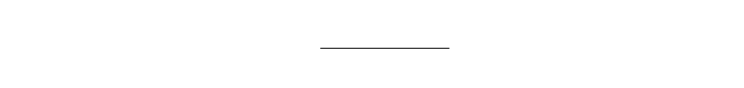
\includegraphics[width=\textwidth]{Figures/SlaterDeterminant1.pdf}
			\label{Slaterdeterminant1}
			\caption{Diagram for the reference state $| \left. \right>$}
		\end{figure}
		While the hole states are represented by vertical lines either going up or down, particle and hole states are depicted by a vertical line. An arrow pointing up relates a particle state, while an arrow pointing down means a hole state. Depicting the two states $\left| \Phi^a \right> $ and $\left| \Phi_i \right>$
		\begin{figure}[H]
			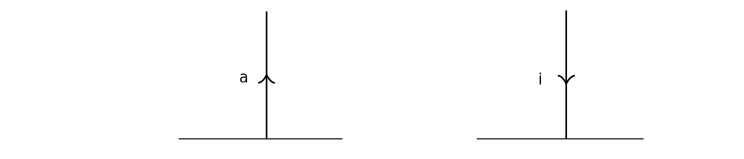
\includegraphics[width=\textwidth]{Figures/SlaterDeterminant2.pdf}
			\label{Slaterdeterminant2}
			\caption{Diagrams for the addition of a particle and a hole state, $\left| \Phi^a \right> $ and $\left| \Phi_i \right> $ respectively}
		\end{figure}
		The ket-variant of the singly excited Slater determinant $\left< \Phi_i^a \right| $ can be drawn as
		\begin{figure}[H]
			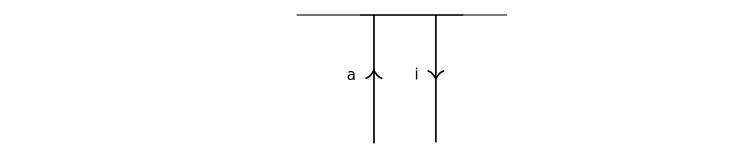
\includegraphics[width=\textwidth]{Figures/SlaterDeterminant3.pdf}
			\label{Slaterdeterminant3}
			\caption{Diagram for the singly excited ket state $\left< \Phi_i^a \right|$}
		\end{figure}
		And the doubly excited states $\left| \Phi_{ij}^{ab} \right>$ can be drawn as
		\begin{figure}[H]
			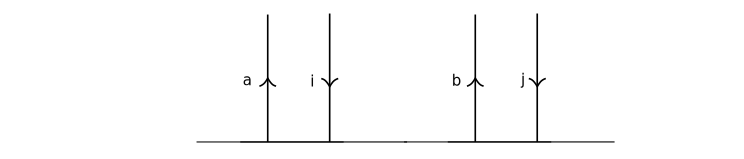
\includegraphics[width=\textwidth]{Figures/SlaterDeterminant4.pdf}
			\label{Slaterdeterminant4}
			\caption{Diagram for the doubly excited bra state $\left| \Phi_{ij}^{ab} \right>$}
		\end{figure}
	\end{section}

	\begin{section}{Operators}
		We need a convention for one-body operators as well. A general one-body operator is given by 
		\begin{align}
			\hat F_N = \sum_{pq} \left< p \right| \hat f \left| q \right> \left\{ \hat p^\dagger \hat q \right\}.
		\end{align}
		We will represent the matrix element $\left< p \right|
                \hat f \left| q \right>$ by a dashed line, while there
                will be one line entering and one line leaving the
                operator due to the annihilation and creation
                operator. Because the operator behaves differently
                depending on whether the general operators $p$ and $q$
                are virtual or occupied states, it can be  written out as 
               four different diagrams as shown in 
                the figure below (adapted from \cite{ShavittAndBartlett})
		\begin{figure}[H]
			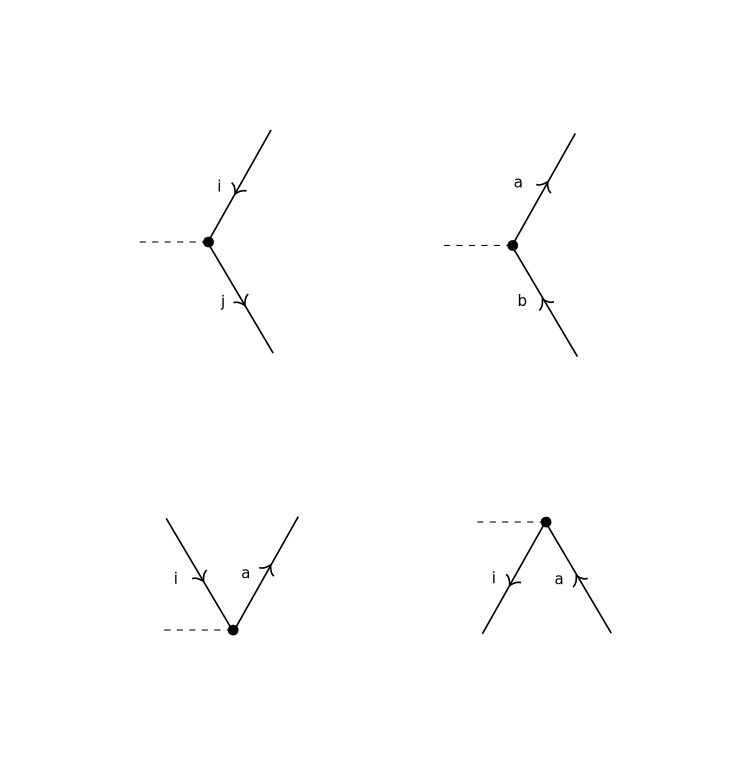
\includegraphics[width=\textwidth]{Figures/OneBodyOperator.pdf}
			\label{OneBodyOperator}
			\caption{Diagrams for four different variants of the one-body operator. From left to right, the operators shown are $\sum_{ij} h_{ij} i^\dagger j $, $\sum_{ab} h_{ab} a^\dagger b$, $\sum_{ai}h_{ai} a^\dagger i$ and $\sum_{ai} h_{ia} i^\dagger a$}
		\end{figure}
		The same logic can be applied to the general two-body operator, given by 
		\begin{align}
			\hat V_N = \frac{1}{4} \sum_{pqrs} \left<pq||rs\right> \left\{ \hat p^\dagger \hat q^\dagger \hat s \hat r \right\}.
		\end{align}
		When we draw this diagram, one will need two outgoing lines representing the creation operators and two incoming lines, representing the annihilation operators. The matrix element will, as for the one-body operator, be drawn as a horizontal \textit{interaction line}
		\begin{figure}[H]
			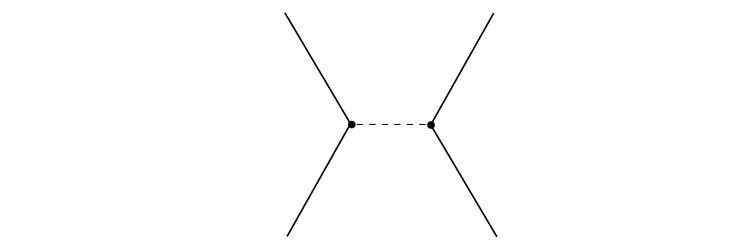
\includegraphics[width=\textwidth]{Figures/TwoBodyOperator0.pdf}
			\caption{two-body operator, showing the horizontal line and four creation or annihilation operators}
			\label{Figure:TwoBodyOperator0}
		\end{figure}
		The left half side of the interaction will represent particle 1, while the right half will represent particle two. We can therefore set up the general relations for the term $\left\{ \hat p^\dagger \hat q^\dagger \hat s \hat r \right\}$
		\begin{align}
			\nonumber \hat p^\dagger &\rightarrow \text{left outgoing line}, \:\:\:\: \hat q^\dagger \rightarrow \text{right outgoing line}, \\
			\nonumber \hat r &\rightarrow \text{left incoming line}, \:\:\:\: \hat s \rightarrow \text{right incoming line}.
		\end{align}
		For the matrix element, we use the rules 
		\begin{align}
			\left< \text{left-out } \text{ right-out } | | \text{ left-in } \text{ right-in } \right>.
		\end{align}
		There should be 16 combinations of particle- and hole-states distributed out between the operators $\hat p^\dagger$, $\hat q^\dagger$, $\hat s$ and $\hat r$, but since some diagrams will be equivalent, we are left with 9 distuingishable diagrams. The equivalent diagrams will be included by a weight factor $2$. 

		\begin{figure}[H]
			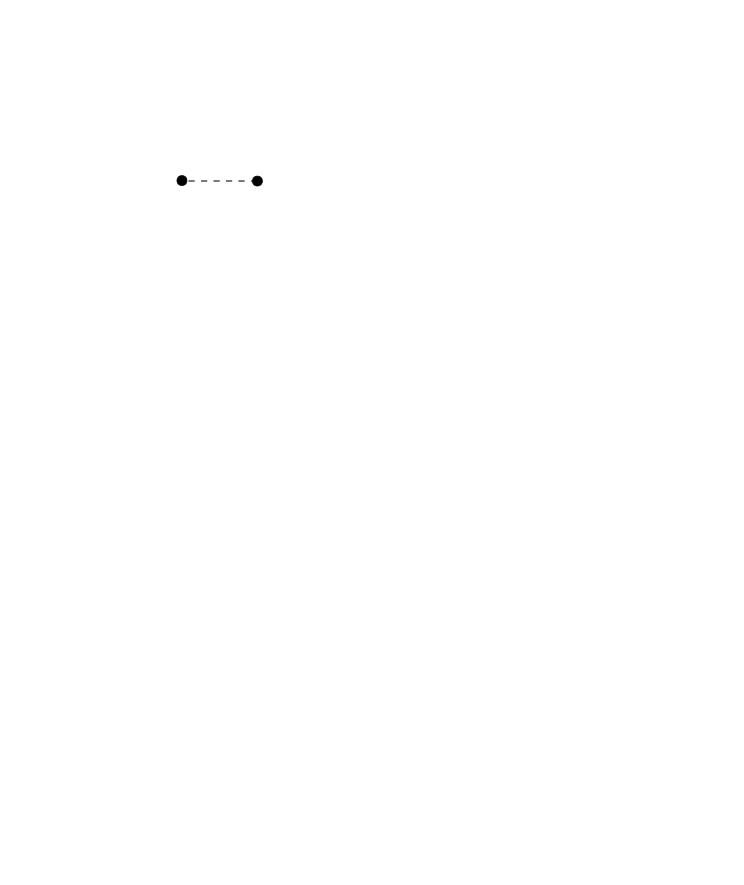
\includegraphics[width=\textwidth]{Figures/TwoBodyOperator.pdf}
			\caption{A figure showing 6 different Goldstone diagrams for the two-body operator. The matrix elements shown, from left to right, are:
			$\left<ab||cd\right>$, $\left<ij||kl\right>$, $\left<ai||bj\right>$, $\left<ab||ci\right>$, $\left<ia||jk\right>$, $\left<ai||bc\right>$.}
			\label{Figure:TwoBodyOperator1}
		\end{figure}

		\begin{figure}[H]
			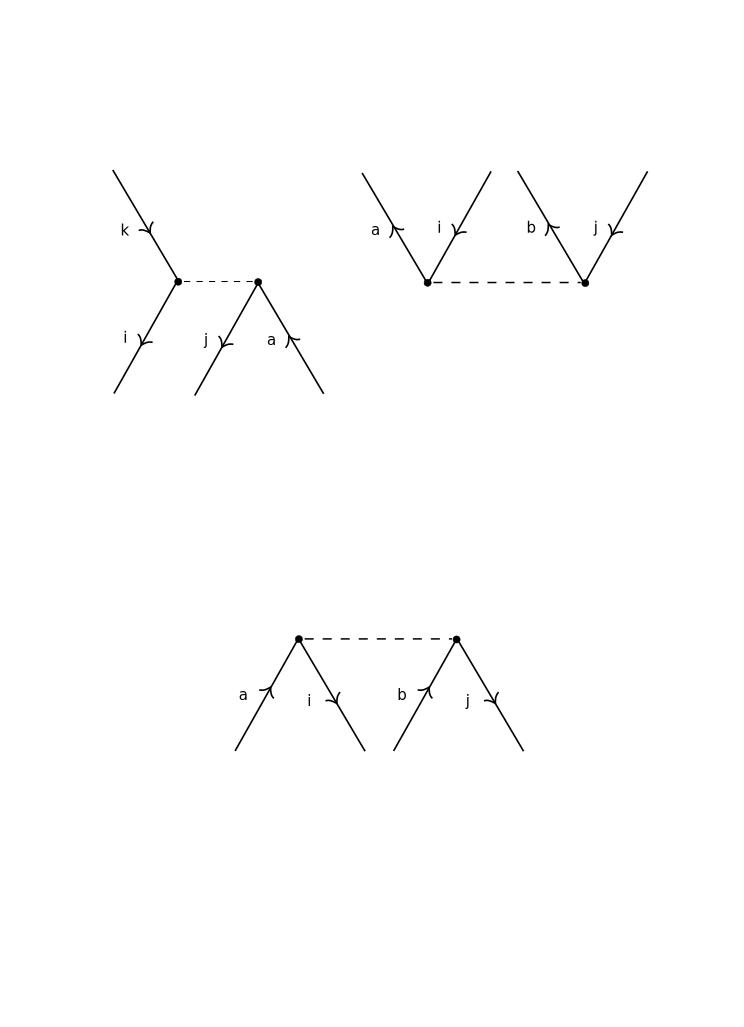
\includegraphics[width=\textwidth]{Figures/TwoBodyOperator2.pdf}
			\caption{A figure showing 3 different Goldstone diagrams for the two-body operator. The matrix elements shown, from left to right, are:
			$\left<ij||ka\right>$, $\left<ab||ij\right>$, $\left<ij||ab\right>$.}
			\label{Figure:TwoBodyOperator2}
		\end{figure}

	\end{section}

	\begin{section}{Contractions and Inner products}
		As seen, contractions are an important part of many-body methods. Representing contractions is easy when using a diagrammatic approach. It is done by connecting the lines between operators and Slater determinants. 
Let us for example consider
the Slater determinant \cite{Audun,ShavittAndBartlett}
		\begin{align}
			\left| \Phi_i^a \right> = \hat a^\dagger \hat i | \left. \right>,
		\end{align}
		and the general one-body operator 
		\begin{align}
			\hat U = \sum_{bc} \left< b | \hat u | c \right> \{ \hat b^\dagger \hat c \}.
		\end{align}
		When the operator $\hat U$ acts on the Slater determinant, the resulting Slater determinant will change 
		\begin{align}
			\hat U \left| \Phi_i^a \right> = \sum_{bc} \left< b | \hat u | c \right> \{ \hat b^\dagger \hat c \} \{ \hat a^\dagger \hat i \} | \left. \right>.
		\end{align}
		We can write this out using the generalized Wick's theorem, noticing that there is only one possible contraction that is non-zero. 
		\begin{align}
			= \left< b | \hat u | c \right> \{ \hat b^\dagger \hat c \hat a^\dagger \hat i \} + \left< b | \hat u | c \right> \{ \hat b^\dagger \contraction{}{\hat c}{}{\hat a^\dagger}
			\hat c \hat a^\dagger \hat i \} = 0 + \left< b | \hat u | c \right> \delta_{ac} \left| \Phi_i^b \right>,
		\end{align}
		which gives
		\begin{align}
			\left< b | \hat u | a \right> \{ \hat b^\dagger \hat i \} | \left. \right> = \left< b | \hat u | a \right> \left| \Phi_i^b \right>
		\end{align}
		The diagrammatic representation of contractions are given in the following figure.
		\newpage 
		\begin{figure}[H]
			\includegraphics[width=\textwidth]{Figures/Contraction.pdf}
			\caption{The diagrammatic representation of a contraction between the  one-body operator and a singly excited Slater determinant.}
			\label{Contraction}
		\end{figure}
		Representing an inner product of two Slater determinants is done by putting together the diagram for a ket state and the diagram for a bra state. Looking at the previous example, taking the expectation value of the general operator $\hat U$, we get 
		\begin{align}
			\left< \Phi_k^d \right| \hat U \left| \Phi_i^a \right>,
		\end{align}
		which can be written out as
		\begin{align}
			\sum_{bj} \left< b | \hat u | c \right> \left< \right. | \{ \hat k^\dagger \hat d \} \{ \hat b^\dagger \hat c \} \{ \hat a^\dagger \hat i \} | \left. \right>.
		\end{align}
		A calculating with the generalized Wick's theorem gives us the result
		\begin{align}
			= \left< d | \hat u | a \right> \delta_{db} \delta_{ac} \delta_{ki}.
		\end{align}
		The expectation are represented in the following figure. 
		\begin{figure}[H]
			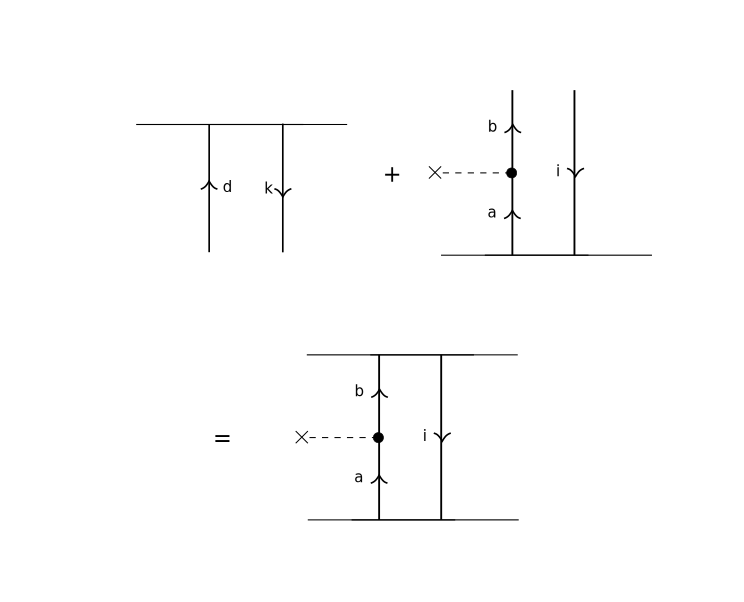
\includegraphics[width=\textwidth]{Figures/InnerProduct.pdf}
			\label{InnerProduct}
			\caption{Diagrammatic representation of the expectation value for a one-body operator between two singly excited Slater determinants.}
		\end{figure}
	\end{section}
	\begin{section}{Interpreting Diagrams}	
		The many-body methods presented in this thesis rely heavily upon operator expressions and contractions. A common way to utilize the toolset presented in this chapter, is to give a visual representation of equations that are less prone to human errors. Using diagrams to perform contractions is by many considered to be more efficient than to perform calculations using Wick's theorem by hand. 

		An important part of using diagrams, is to have a consistent toolset to translate diagrams into mathematical expressions. These tools exist, see for example \cite{ShavittAndBartlett}, and the implementation of perturbation theory for the pairing model presented in this thesis. 
	\end{section}

\end{chapter}



\begin{chapter}{Many-Body Methods}
	We define an ansatz for the ground state, $\left| \Phi_0 \right>$ as a Slater determinant consisting of the single-particle states, $\left| \phi_i \right>$
	\begin{align}
		\ket{\Psi} \approx \ket{\Phi_0} = 	\frac{1}{ \sqrt{N!} } \left|\begin{matrix}
			\phi_1(\mathbf{x}_1) & \phi_2(\mathbf{x}_1) & ... & \phi_N(\mathbf{x}_1) \\
			\phi_1(\mathbf{x}_2) & \phi_2(\mathbf{x}_2) & ... & \phi_N(\mathbf{x}_2) \\
			... & & & \\
			\phi_1(\mathbf{x}_N) & \phi_2(\mathbf{x}_N) & ... & \phi_N(\mathbf{x}_N),
		\end{matrix} \right|
	\end{align}
	which can be rewritten using second quantization
	\begin{align}
		\left| \Phi_0 \right> = \left( \prod_{i \leq F} \hat i^\dagger \right) \left| 0 \right> = |\left.  \right>.
	\end{align}
	Typically one chooses well-known and mathematically simple single-particle states that are easy to implement. In this thesis, I have used a free particle wave function as single-particle states for infinite matter. Using this basis, I obviously fail to incorporate the interaction between electrons since $\phi_1$ remains unchanged if I also add $\phi_2$. This can be solved by using a smarter basis, which is the goal of Hartree-Fock. Through an iterative method, the single-particle basis is modified so as to to get an improved representation of the ground state. This can be viewed as incorporating the interaction as a \textit{mean field} approximation. 

	I will in this thesis present, and use, three \textit{post Hartree-Fock} methods. These are \textit{Full Configuration Interaction Theory}, \textit{Many-Body Perturbation Theory} and \textit{Coupled Cluster Theory}, where the latter is the main focus of my thesis. These methods aim to compute the \textit{Correlation Energy} as presented in the chapter on Second Quantization. It is common to first implement the Hartree-Fock method, providing the most precise reference energy. 

	\begin{section}{Full Configuration Interaction Theory}
		The first \textit{Post Hartree-Fock} method to be presented is  \textit{Full Configuration Interaction theory}. We expand the true wave function as a linear combination of the ground state ansatz and all possible excitations
		\begin{align}
			\left| \Psi \right> = C_0 \left| \Phi_0 \right> + \sum_{ai} C_i^a \left| \Phi_i^a \right> + \sum_{abij} C_{ij}^{ab} \left| \Phi_{ij}^{ab} \right> + ... ,
		\end{align}
		which can be rewritten in terms of a \textit{correlation operator}
		\begin{align}
			\left| \Psi \right> = ( C_0 + \hat C) \left| \Phi_0 \right>,
		\end{align}
		with
		\begin{align}
			\hat C = \sum_{ai} C_i^a \hat a^\dagger \hat i + \sum_{abij} C_{ij}^{ab} \hat a^\dagger \hat b^\dagger \hat j \hat i + ... \; .
		\end{align}
		We can name the terms such that
		\begin{align}
			\hat C = \hat C_1 + \hat C_2 + ... \; .
		\end{align}
		We use intermediate normalization, which gives us $C_0 = 1$, such that we get the relation
		\begin{align}
			\left< \Psi | \Phi_0 \right> = C_0 \left< \Phi_0 | \Phi_0 \right> = 1.
		\end{align}
		We can now rewrite $\left| \Psi \right>$
		\begin{align}
			\left| \Psi \right> = (1 + \hat C) \left| \Phi_0 \right> .
			\label{equation:FCI}
		\end{align}
		To simplify the notation, we can write the equation in terms of $P$ and $H$, which symbolizes all possible chains of creation and annihilation operators
		\begin{align}
			\left| \Psi \right> = \sum_{PH} C_H^P \left| \Phi_H^P \right> = \left( \sum_{PH} C_H^P \hat A_H^P \right) \left| \Phi_0 \right>  .
		\end{align}
		We are working with orthonormal states, meaning that 
		\begin{align}
			\left< \Psi | \Psi \right> = \sum_{PH} \left| C_H^P \right|^2 = 1.
		\end{align}
		The only thing left now, is defining how to compute the correlation energy. We write the expression for the energy as
		\begin{align}
			E = \left< \right. \Psi | \hat H | \Psi \left. \right> = \sum_{PHP'H'} (C^P_H)^* \left< \right. \Phi_H^P | \hat H | \Phi_{H'}^{P'} \left. \right> C_{H'}^{P'} .
		\end{align} 
		
		\begin{subsection}{The Hamiltonian Matrix}
			We can build a Hamiltonian matrix consisting of all possible combinations of Slater determinants, i.e. all possible combinations of $P,H$ and $P',H'$. The matrix elements will be the expectation value for the Hamiltonian, $\hat{\mathcal{H}}$, with respect to the given Slater determinants. The matrix is set up with the inner products of the following excited states
			\begin{align}
				\begin{pmatrix}
							& 0p - 0h & 1p - 1h & 2p - 2h & 3p - 3h & 4p-4h & ... & Np - Nh \\ 
					0p - 0h & x 	  & x 		& x 	  & 0 		& 0 	& 0	   & 0 		\\		
					1p - 1h & x 	  & x 		& x 	  & x  		& 0 	& 0    & 0 		\\
					2p - 2h & x 	  & x 		& x 	  & x  		& x		&\cdots& 0		\\
					3p - 3h & 0 	  & x 		& x 	  & x  		& x 	&\cdots& 0 		\\
					4p - 4h & 0		  & 0 		& x 	  & x 		& x 	&\cdots& 0		\\
					\vdots 	& 0  	  & 0 	    & \vdots  & \vdots  & \vdots&\ddots& \vdots \\
					Np - Nh & 0 	  & 0		& 0 	  & 0 		& 0		&\hdots& x
				\end{pmatrix}. 
			\end{align}
			Above is an example of a general Hamiltonian matrix, $\mathcal{H}$, set up for an $N$-particles, $N$-holes, basis. One can notice that many matrix elements are zero. This is because the Hamiltonian only have a two-particle interaction term. If we have performed Hartree-Fock calculations, or start out with a Hartree-Fock basis, we have shifted the basis so that all matrix elements of the type
			\begin{align}
				\left< 0p-0h \right| \hat H \left| 1p-1h \right> = \left< 1p-1h \right| \hat H \left| 0p-0h \right> = 0, 
			\end{align}
			will be equal to zero. This gives a shifted Hamiltonian matrix, $\hat{\mathcal{H}}$, where the inner products are changed. The shifted matrix is given as 
			\begin{align}
				\left(  \begin{matrix}
							& 0p - 0h & 1p - 1h & 2p - 2h & 3p - 3h & 4p - 4h & ... & Np - Nh \\ 
					0p - 0h & \tilde x& 0       & \tilde x& 0 		& 0 	  & 0	 & 0 		\\		
					1p - 1h & 0 	  & \tilde x& \tilde x& \tilde x& 0 	  & 0    & 0 		\\
					2p - 2h & \tilde x& \tilde x& \tilde x& \tilde x& \tilde x&\cdots& 0		\\
					3p - 3h & 0 	  & \tilde x& \tilde x& \tilde x& \tilde x&\cdots& 0 		\\
					4p - 4h & 0		  & 0 		& \tilde x& \tilde x& \tilde x&\cdots& 0		\\
					... 	& 0  	  & 0 	    & \vdots  & \vdots  & \vdots  &\ddots& \vdots\\
					Np - Nh & 0 	  & 0		& 0 	  & 0 		& 0		  &\cdots& \tilde x
				\end{matrix} \right)
			\end{align}
			To find the ground state correlation energy,
                        the normal procedure is to diagonalize the
                        Hamiltonian matrix through diagonalization
                        algorithms. If we have a finite size Hilbert
                        space, we can set up a finite Hamiltonian
                        matrix which, when diagonalized, will provide
                        us with the exact ground state correlation
                        energy.

			Unfortunatly, Full Configuration
                        Interaction Theory is computationally
                        costly. The Hamiltonian matrix will grow
                        exponentially fast for large Hilbert spaces,
                        which both increases the memory usage
                        dramatically and increases the prosessing
                        power associated with diagonalizing the
                        matrix. For infinite and very large Hilbert
                        spaces, one can truncate the number of
                        excitations at some level to reduce the size
                        of Hamiltonian matrix. I will later refer to
                        this as just \textit{Configuration Interaction
                          theory}.
		\end{subsection}

		\begin{subsection}{Computational cost}
			As an example on how costly  full configuration interaction theory can be \cite{MHJFCI}, we look at the oxygen nucleus. For a system consisting of $N$ states and $n$ particles, the total number of unique Slater determinants is given by 
			\begin{align}
				\binom{N}{n} = \frac{n!}{(n-N)!N!}.
				\label{FCI1}
			\end{align}
			Looking at the oxygen-16, we have $8$ protons and $8$ neutrons. If we only include the first major shells, we have a total of $40$ states that the neutrons and protons can occupy \cite{MHJFCI}. Using equation (\ref{FCI1})
			\begin{align}
				\binom{40}{8} = \frac{40!}{32!8!} \approx 10^9,
			\end{align}
			for both the protons and the neutrons. Multiplying them together, we get 
			\begin{align}
				10^9 10^9 = 10^{18},
			\end{align}
			Slater determinants for the whole system. This shows how fast the dimensionality explodes! 

		\end{subsection}

	\end{section}	

	\begin{section}{Many-body Perturbation Theory}
		Many-body perturbation theory presents a non-iterative approach to approximating the ground state energy. The approach is similar to previous methods. We start by splitting the Hamiltonian into a solvable part and a perturbation 
	 	\begin{align}
	 		\hat H = \hat H_0 + \hat V,
	 	\end{align}
	 	where we have chosen our basis such that
	 	\begin{align}
	 		\hat H_0 \left| \Psi_0 \right>  = W_0 \left| \Psi_0 \right>.
	 	\end{align}
	 	We also split the basis
	 	\begin{align}
	 		\left| \Psi_0 \right> = \left| \Phi_0 \right> + \sum_i^{\infty} c_i \left| \phi_i \right>.
	 	\end{align}
	 	Assuming intermediate normalization
	 	\begin{align}
	 		\left< \Phi_0 | \Psi_0 \right> = 1,
	 	\end{align}
		we can calculate the total exact energy
	 	\begin{align}
	 		E = \left< \Phi_0 \right| \hat H_0 \left| \Psi_0 \right> + \left< \Phi_0 \right| \hat V \left| \Psi_0 \right>,
	 	\end{align}
	 	where we know that
	 	\begin{align}
	 		 \left< \Phi_0 \right| \hat H_0 \left| \Psi_0 \right>  = W_0.
	 	\end{align}
	 	We get the correlation energy
	 	\begin{align}
	 		E - W_0 = \Delta E = \left< \Phi_0 \right| \hat V \left| \Psi_0 \right>.
	 	\end{align}
	 	We will usually aim to compute the correlation energy, $\Delta E$, when doing MBPT. 

	 	\begin{subsection}{General derivation of Many-Body Particle Theory equations}
	 		Looking at the equation
	 		\begin{align}
	 			\hat V \left| \Psi_0 \right> = \hat H \left| \Psi_0 \right> - \hat H_0 \left| \Psi_0 \right> ,
	 		\end{align}
	 		we reorganize and add the term $\omega \left| \Psi_0 \right>$ on both sides
	 		\begin{align}
	 			\hat V \left| \Psi_0 \right> + \omega \left| \Psi_0 \right> - \hat H \left| \Psi_0 \right> = \omega \left| \Psi_0 \right> - \hat H_0 \left| \Psi_0 \right> .
	 		\end{align}
	 		Remembering that $\hat H \left| \Psi_0 \right> = E\left| \Psi_0 \right> $, we get 
	 		\begin{align}
	 			\left| \Psi_0 \right> = \frac{ \hat V + \omega - E }{\omega - \hat H_0} \left| \Psi_0 \right>.
	 			\label{pert_1}
	 		\end{align}
	 		Before continuing, we introduce the operators $\hat P$ and $\hat Q$, such that
	 		\begin{align}
	 			\left| \Psi_0 \right> = \hat P \left| \Psi_0 \right> + \hat Q \left| \Psi_0 \right> 
	 			&= \left| \Phi_0 \right> \left< \Phi_0 \middle| \Psi_0 \right> + \sum_i \left| \Phi_i \right> \left< \Phi_i \middle| \Psi_0 \right> ,
	 			\label{pert_2} \\
	 			&= \left| \Phi_0 \right> + \chi ,
	 		\end{align}
	 		which gives
	 		\begin{align}
	 			\left| \Phi_0 \right> = \hat P \left| \Psi_0 \right> \;\;\;\; \chi = \hat Q \left| \Psi_0 \right> .
	 			\label{pert_3}
	 		\end{align}
	 		Using $\hat R(\omega) = \frac{\hat{Q}}{\left( \omega - \hat H_0 \right)}$ and multiplying both sides with $\hat Q$ from the left in equation (\ref{pert_1}) we attain
	 		\begin{align}
	 			\hat Q \left| \Psi_0 \right> = \hat R(\omega) \left( \hat V + \omega - E \right) \left| \Psi_0 \right>.
	 		\end{align}
	 		Using equations (\ref{pert_2}) and (\ref{pert_3}), we get
	 		\begin{align}
	 			\left| \Psi_0 \right> = \left| \Phi_0 \right> + \hat R(\omega) \left( \hat V + \omega - E \right) \left| \Psi_0 \right>.
	 		\end{align}
	 		This sets up an iterative scheme, where we need to know $\left| \Psi_0 \right>$ before we can calculate $\left| \Psi_0 \right>$. We can substitute the state $\left| \Psi_0 \right>$ on the right hand side with the entire right hand side. This results in an infinite sum provided the series converges
	 		\begin{align}
	 			\left| \Psi_0 \right> = \sum_0^\infty \left\{ \hat R(\omega) (\hat V + \omega - E) \right\}^m \left| \Phi_0 \right>.
	 		\end{align}
	 		The right hand side does include the energy, $E$, which must be computed using $ E = W_0 + \Delta E$, and
	 		\begin{align}
	 			\Delta E = \left< \Phi_0 \right| \hat V \left| \Psi_0 \right> 
	 			= \sum_0^\infty \left< \Phi_0 \right| \hat V \left[ \hat R(\omega) (\hat V - E + \omega) \right]^m \left| \Phi_0 \right>.
	 		\end{align}
	 	\end{subsection}

	 	\begin{subsection}{Equations for Rayleigh-Schr\"{o}dinger Perturbation Theory}
	 		We can interpret $\omega$ in different ways. I here present the Rayleigh-Schr\"{o}dinger Perturbation Theory which postulates that
	 		\begin{align}
	 			\omega = E_0^{(0)},
	 		\end{align}
	 		such that we get the expression for the resolvent
	 		\begin{align}
	 			\hat R_0 = \frac{\hat Q}{E_0^{0} - \hat H_0}.
	 		\end{align}
	 		This gives the expression for $\left| \Psi_0 \right>$
	 		\begin{align}
	 			\left| \Psi_0 \right> = \frac{ \hat V - \Delta E }{\omega - \hat H_0} \left| \Psi_0 \right>,
	 		\end{align}
	 		and we get the final equation for the wave function 
	 		\begin{align}
	 			\left| \Psi_0 \right> = \sum_0^\infty \left\{ \hat R(\omega) (\hat V + - \Delta E) \right\}^m \left| \Phi_0 \right>.
	 		\end{align}
	 		The correlation energy can be calculated by 
	 		\begin{align}
	 			\Delta E = \sum_0^\infty \left< \Phi_0 \right| \hat V \left[ \hat R(\omega) (\hat V - \Delta E) \right]^m \left| \Phi_0 \right> .
	 		\end{align}
	 		Taking a closer look at the energy-equations, we find that we can write the first orders as
	 		\begin{align*}
	 			E^{(1)} &= \left< \Phi_0 \right| \hat V \left| \Phi_0 \right>  = V_{00},\\
	 			E^{(2)} &= \left< \Phi_0 \right| \hat V \hat R_0 \hat V \left| \Phi_0 \right>, \\
	 			E^{(3)} &= \left< \Phi_0 \right| \hat V \hat R_0 (\hat V - E^{(1)})  \hat R_0 \hat V \left| \Phi_0 \right>, \\
	 			E^{(4)} &= \left< \Phi_0 \right| \hat V \hat R_0 (\hat V - E^{(1)})  \hat R_0 (\hat V - E^{(1)}) \hat R_0 \hat V \left| \Phi_0 \right> 
	 					- E^{(2)} \left< \Phi_0 \right| \hat V \hat R_0^2 \hat V \left| \Phi_0 \right>.
	  		\end{align*}
	  		Because of the frequent appearance, we can rewrite $\hat V - E^{(1)}$ as
	  		\begin{align}
	  			\hat \Omega = \hat V - E^{(1)} = \hat V - \left< \Phi_0 \right| \hat V \left| \Phi_0 \right>.
	  		\end{align}
	  		We name this new variable the wave operator, and rewrite the equations in a simpler form 
	  		\begin{align*}
	 			E^{(1)} &= \left< \Phi_0 \right| \hat V \left| \Phi_0 \right>  = V_{00},\\
	 			E^{(2)} &= \left< \Phi_0 \right| \hat V \hat R_0 \hat V \left| \Phi_0 \right>, \\
	 			E^{(3)} &= \left< \Phi_0 \right| \hat V \hat R_0 \hat \Omega \hat R_0 \hat V \left| \Phi_0 \right>, \\
	 			E^{(4)} &= \left< \Phi_0 \right| \hat V \hat R_0 \hat \Omega  \hat R_0 \hat \Omega \hat R_0 \hat V \left| \Phi_0 \right> 
	 					- E^{(2)} \left< \Phi_0 \right| \hat V \hat R_0^2 \hat V \left| \Phi_0 \right>.
	 			\label{MBPT equations}
	  		\end{align*}
	  		I am, in this thesis, concerned with calculating the correlation energy, and these four equations will be implemented for the Pairing model. 
	 	\end{subsection}
	\end{section}

	\begin{section}{Linked Diagram theorem}
		The linked diagram theorem is an important theorem, presented by Goldstone in 1957 \cite{ShavittAndBartlett,Goldstone} which leads to the cancellation of all unlinked diagrams in Rayleigh-Schr\"{o}dinger perturbation theory.

		The theorem states that the wave function and the energy can be expressed as a sum of linked diagrams \textit{only}, reducing the equations to 
		\begin{align}
			E^{(n)} = \left< \right. | \hat W (\hat R_0 \hat W)^{n-1} \left. | \right>_L, \\
			\left| \Psi^{(n)} \right> = \left[ (\hat R_0 \hat W)^n |\left.\right>  \right]_L.
		\end{align}

	\end{section}

	\begin{section}{Hartree-Fock calculations}
 		When doing Hartree-Fock calculation, we conduct a
                change of the basis, and instead of expanding our
                Hamiltonian, we vary the wave function to minimize the
                energy. We name the original basis by greek letters
                and the new basis by latin letters. The original basis
                should be chosen such that we can calculate its
                expectation value.
 		\begin{align}
 			\left< \Phi_0 \right| \hat H \left| \Phi_0 \right> = E^{\text{HF}}.
 		\end{align}
 		The variational principle ensures that 
 		\begin{align}
 			E^{\text{HF}} > 0 .
 		\end{align}
 		We introduce a change of basis
 		\begin{align}
 			\left| \psi_a \right> = \sum_{\lambda} C_{a\lambda} \left| \psi_{\lambda} \right>.
 		\end{align}
 		Varying $C_{p\lambda}$, we can search for the basis which yields the lowest energy. We start by rewriting $E^{HF}$ as a functional
 		\begin{align}
 			E\left[ \psi \right] = \sum_{a=1}^N \left< a \right| h \left| a \right> + \frac{1}{2} \sum_{ab}^N \left< ab \right| v \left| ab \right>.
  		\end{align}
  		Rewriting it in terms of the original basis (greek letters), we get the energy functional given as
  		\begin{align}
  			E\left[ \psi \right] = \sum_{a=1}^N \sum_{\alpha \beta} C_{a \alpha}^* C_{a \beta} \left< \alpha \right| h \left| \beta \right> + \frac{1}{2} \sum_{ab}^N \sum_{\alpha \beta \gamma \delta} C_{a \alpha}^* C_{b \beta}^* C_{a \gamma} C_{b \delta} \left< \alpha \beta \right| v \left| \gamma \delta \right>.
  		\end{align}
  		To find the minima, we introduce a Lagrange multiplier before differentiating with respect to $C_{a  \alpha}^*$. This will give N equations, one for each state $a$. The equations are given by
  		\begin{align}
  			\sum_{\beta} C_{a \beta} \left< \alpha \right| h \left| \beta \right> + \sum_b^N \sum_{\beta \gamma \delta} C_{b \beta}^* C_{b \delta} C_{a \gamma} \left< \alpha \beta \right| v \left| \gamma \delta \right> = \epsilon_a C_{a \alpha}.
  		\end{align}
  		Defining
  		\begin{align}
  			h_{\alpha \gamma}^{\text{HF}} = \left< \alpha \right| h \left| \gamma \right> + \sum_{b=1}^N \sum_{\beta \delta} C_{b \beta}^* C_{b \delta} \left< \alpha \beta \right| v \left| \gamma \delta \right> ,
  		\end{align}
  		we get the short hand iterative equations to be solved 
  		\begin{align}
  			\sum_{\gamma} h_{\alpha \gamma}^{\text{HF}} C_{a \gamma} = \epsilon_{a} C_{a \alpha}.
  		\end{align}
  		A natural starting point for the constants, $C$, is to set
  		\begin{align}
  			C_{a\lambda} = \delta_{a \lambda},
  		\end{align}
  		which means that the first guess is to use the original greek basis. 
 	\end{section}

\end{chapter}



\begin{chapter}{Coupled-Cluster Theory} 
	Coupled-cluster theory is similar to full configuration
        interaction theory. Coupled-cluster theory is a
        post-Hartree-Fock method.
        The goal of Coupled-cluster theory is to
        improve the ansatz by including a set of excitations that can be summed to infinite order. Coester
        and K\"ummel initially developed the ideas that led to the
        coupled-cluster theory in the late 1950's \cite{MHJonline}.
 	
 	\begin{section}{The Exponential Ansatz}
 		The basic idea of Coupled-cluster theory is to express the true wave function as an exponential operator working on the Slater determinant \cite{ShavittAndBartlett,MHJonline,Crawford}
 		\begin{align}
	 		\ket{\Psi} \approx e^{\hat T} \ket{\Phi_0}.
	  	\end{align}
	  	The operator $\hat T$, is a sum of the excitation operators, also known as cluster operators
	  	\begin{align}
	  		\hat T = \hat T_1 + \hat T_2 + \hat T_3 + ... + \hat T_N,
	  	\end{align}
	  	where the operators are defined as
	  	\begin{align}
	  		T_1 &= \sum_{ia} t_i^a \hat a_a^{\dagger} \hat a_i, \\
	  		T_2 &= \frac{1}{2} \sum_{ijab} t_{ij}^{ab} \hat a_a^{\dagger}\hat a_b^{\dagger} \hat a_j \hat a_i, \\
	  		T_N &= \left(\frac{1}{n!}\right)^2 \sum_{ij..ab..}^n t_{ij..n}^{ab..n} \hat a_a^{\dagger}\hat a_b^{\dagger} ...\hat a_n^{\dagger} \hat a_n ... \hat a_j \hat a_i, \\
	  	\end{align}
	  	which we will see is similar to configuration interaction theory.
	\end{section}

	\begin{section}{Comparison with Configuration Interaction}
	  	By doing an expansion of the exponential operator, we can rewrite it as
	  	\begin{align}
	  		e^{\hat T} = 1 + \hat T + \frac{\hat T^2}{2!} + \frac{\hat T^3}{3!} + \cdots.
	  	\end{align}
	  	Calculating the terms and organizing them in terms of total excitations, we can write the exponential operator as 
	  	\begin{align}
	  		e^{\hat T} = \left( 1 \right)  + \left( \hat T_1 \right) + \left( \hat T_2 + \frac{\hat T_1^2}{2} \right) + \left( \hat T_3 + \hat T_1 \hat T_2 + \frac{\hat T_1^3}{6} \right) + \cdots .
	  	\end{align}	
	  	Remembering the equation for configuration interaction, given by equation (\ref{equation:FCI})
	  	\begin{align*}
	  		\ket{\Psi_{CI}} = (1 + \hat C) \ket{\Phi_0}, 
	   	\end{align*}
	   	where
	  	\begin{align*}
	  		\hat C = \hat C_1 + \hat C_2 + ... =  \sum_{ia} c_i^a a_a^{\dagger} a_i + \frac{1}{4} \sum_{ijab} c_{ij}^{ab} a_a^{\dagger} a_b^{\dagger} a_j a_i + ...
	   	\end{align*}
	   	By comparing configuration interaction with coupled-cluster theory, we see that we can write
	   	\begin{align}
	   		\hat C_0 = 1 \:\:\:\:\:\:\:, \hat C_1 = \hat T_1 ,
	   	\end{align}
	   	\begin{align}
	   		\hat C_2 = \hat T_2 + \frac{1}{2} T_1^2,
	   	\end{align}
	   	and 
	   	\begin{align}
	   		\hat C_3 = \hat T_3 + \hat T_1 \hat T_2 + \frac{\hat T_1^3}{6}.
	   	\end{align}
	   	The difference we notice, is that coupled-cluster introduces a mixing of excitation operators for every level of total excitations. 
 	\end{section}

	\begin{section}{Truncating the Exponential Ansatz}
	  	By including infinite terms, this expansion will represent the true wave function, but the equations cannot be computed unless they are truncated at some point. 
	  	\begin{enumerate}
	  		\item By including only $\hat T = \hat T_1$, we are doing coupled-cluster singles, short-handed by \textit{CCS}
	  		\item By truncating the equations at double excitations, $\hat T = \hat T_1 + \hat T_2$, we are doing coupled-cluster singles and doubles, with the short-hand given by \textit{CCSD}
	  		\item By truncating the equations at triple excitations, $\hat T = \hat T_1 + \hat T_2 + \hat T_3$, we are doing coupled-cluster singles, doubles and 		triples, \textit{CCSDT}
	  		\item four excitations are called quadruples, and so on
	  	\end{enumerate}

	  	We introduce a new operator, $\overline H$, given by 
	  	\begin{align}
	  		\overline H = e^{-\hat T} \hat H e^{\hat T} .
	  	\end{align}
	  	When calculating the energy, we look at the expectation value for the Hamiltonian 
	  	\begin{align}
	  		\left< \Phi_0 \right| e^{-\hat T} \hat H e^{\hat T} \left| \Phi_0 \right> = \left< \Phi_0 \right| \overline H \left| \Phi_0 \right> = E.
	  	\end{align}
	  	By subsequent left-projection of various excited states, we get amplitude equations
	  	\begin{align}
	  		\left< \Phi_{ij\cdots}^{ab\cdots} \right| \overline H \left| \Phi_0 \right> = 0.
	  	\end{align}
	  	We have now decoupled the amplitude equations from the energy equations, reducing the complexity of a coupled-cluster solver. The energy-equation is a function of the amplitudes $t_i, t_j, \cdots$ and $t_a, t_b, \cdots$, which can now be found through a different set of iterative equations. We have introduced the similarity transformed Hamiltonian, which can be significantly simplified using the Baker-Campbell-Hausdorff formula \cite{Crawford}
	  	\begin{align}
	  		\overline H = e^{-\hat T} \hat H e^{\hat T} =& \hat H + [ \hat H, \hat T] + \frac{1}{2!} [[\hat H, \hat T], \hat T] \\ + &\frac{1}{3!} [[[ \hat H, \hat T ], \hat T ], \hat T ] + \frac{1}{4!} [[[[\hat H, \hat T], \hat T], \hat T], \hat T] + \cdots \nonumber .
	  	\end{align}
	  	At first glance, this equation does not look like a simplification, but based on properties on the system, we can truncate this expansion. The cluster operators, $\hat T_1, \hat T_2, \hat T_3, \cdots$ commute with each other, but they do not generally commute with the Hamiltonian operator. Consider the general commutation of the one-body Hamiltonian and the $T_1$ cluster operator
	  	\begin{align}
	  		[\hat H_0, \hat T_1] = [\hat p^\dagger \hat q, \hat a^\dagger \hat i] = \hat p^\dagger \hat q \hat a^\dagger \hat i - \hat a^\dagger \hat i \hat p^\dagger \hat q.
	  	\end{align}
	  	We can use the anti-commutator relations to rewrite two terms on the right-hand side
	  	\begin{align}
	  		\hat p^\dagger \delta_{qa} \hat i - \hat a^\dagger \delta_{ip} \hat q.
	  	\end{align}
	  	Because $p$ and $q$ are summed over of all possible states, and are not limited to virtual or occupied states, we cannot explicitly state that the Kronecker delta functions $\delta_{qa}$ or $\delta_{ip}$ are either $0$ or $1$. 

	  	Because the cluster operators commute, to get a non-zero result, the Hamiltonian must create one Kronecker-delta function for each of the participating cluster operators. For every system in this thesis, we are only working with a two-body Hamiltonian, so a commutation with more than four cluster operators must provide zero. We will get a natural truncation, that holds for both the energy and amplitude equations. This is true for all systems that have a two-body Hamiltonian. We now write the similarity transformed Hamiltonian as
	  	\begin{align}
	  		\overline H = e^{-\hat T} \hat H e^{\hat T} = \hat H &+ [ \hat H, \hat T] + \frac{1}{2!} [[\hat H, \hat T], \hat T] + \frac{1}{3!} [[[ \hat H, \hat T ], \hat T ], \hat T ] \\  &+ \frac{1}{4!} [[[[\hat H, \hat T], \hat T], \hat T], \hat T] \nonumber.
	  	\end{align}

	\end{section}  	

	\begin{section}{The Variational Principle}
		Using a variational method comes with great advantages. One can be sure to have calculated an upper boundary to the energy, but the coupled-cluster energy equation do not conform to any variational conditions \cite{Crawford}. However, the exponential ansatz does allow for another way of setting up the energy equation
		\begin{align}
			E_{\text{exact}} \leq E = \frac{\left< \Phi_0 \right| (e^{\hat T})^\dagger \hat H e^{\hat T} \left| \Phi_0 \right>}{\left< \Phi_0 \right| (e^{\hat T})^\dagger \hat H e^{\hat T} \left| \Phi_0 \right>} = \frac{\left< \Psi \right| \hat H \left| \Psi \right>}{\left< \Psi \right| \hat H \left| \Psi \right>},
		\end{align}
		which is variational. Unfortunately, one can not apply
                the same logic of natural truncation to the
                variational coupled-cluster energy. 
	\end{section}

  	\begin{section}{Size-Extensivity}
  		It can be important to have a wave function that scales with size. Imagine two particles, $X$ and $Y$, with infinite separation, meaning that they do not interact. This means we should be able to write the total energy as
  		\begin{align}
  			E = E_X + E_Y.
  		\end{align}
  		Rewriting the cluster operators in terms of the two particles
  		\begin{align}
  			\hat T = \hat T_X + \hat T_Y,
  		\end{align}
  		the wave function can be rewritten as 
  		\begin{align}
  			\ket{\Psi}_{CC} = e^{\hat T_X + \hat T_Y} \ket{\Phi_0} = e^{\hat T_X} e^{\hat T_Y} \ket{\Psi_0}.
  		\end{align}
  		Since we can write the reference state as a product of the two separated parts, we are able to write
  		\begin{align}
  			E_{CC} = E_{CC}^X + E_{CC}^Y.
  		\end{align}
  		For Configuration Interaction, multiplicative separability is not possible
  		\begin{align}
  			\Psi_{CI} = \left(1 + \hat C\right) \Phi_0 = \left( 1 + \hat C_x + \hat C_y \right) \Phi_0,
  		\end{align}
  		which cannot be rewritten as two separable parts. This means the coupled-cluster theory produces a \textit{size-extensive} energy, contrary to full configuration interaction. A size-extensive system will scale perfectly with the size of the system, regardless of the interaction between the particles.

  	\end{section}

  	\begin{section}{The Coupled-Cluster Doubles Equations}
  		We need to truncate the cluster operator, $\hat T$, and the approximation used in this thesis, is to only allow 2p-2h excitations. This is normally referred to as the coupled-cluster doubles equations, or CCD. We can rewrite the operator as \cite{MHJonline}
  		\begin{align}
  			\hat T \approx \hat T_2.
  		\end{align}
  		The wave function will be approximated by 
  		\begin{align}
  			\left| \Psi_0 \right> \approx \left| \Psi_{\text{CCD}} \right> = e^{\hat T_2} \left| \Phi_0 \right>.
  		\end{align}
  		Inserting this ansatz into the Hamiltonian expectation value, we get
  		\begin{align}
  			\left< \Phi_0 \right| e^{-\hat T_2} \hat H e^{\hat T_2} \left| \Phi_0 \right> ,
  		\end{align}
  		which will have the natural truncation at 
  		\begin{align}
  			\left< \Phi_0 \right|  \hat H (1 + \hat T_2) \left| \Phi_0 \right> = E_{\text{CCD}}.
  		\end{align}
  		This leads up to the energy equation
  		\begin{align}
  			E_{\text{CCD}} = E_{\text{ref}} + \frac{1}{4} \sum_{abij} \left<ij|\hat v|ab\right> t_{ij}^{ab},
  		\end{align}
  		with the reference energy defined as 
  		\begin{align}
  			E_{ref} = \sum_i \left< i \right| \hat h_0 \left| j\right> + \sum_{ij} \left<ij\middle|\hat v\middle|ij\right> + \frac{1}{2}Av_0.
  		\end{align}
  		We have used $v_0$, which is a constant, nonzero for the finite electron gas. The second part of the energy, is known as the correlation energy. It is given by
  		\begin{align}
  			\Delta E_{CCD} = \frac{1}{4} \sum_{ijab}\left<ij\middle|\hat v\middle|ab\right> t_{ij}^{ab}.
  		\end{align}
  		The computation of this correlation energy is the goal of the coupled-cluster theory. This depends on the amplitudes $t_{ij}^{ab}$ and we need the corresopnding amplitude equations, found by
  		\begin{align}
  			\left< \Phi_{ij}^{ab} \right| e^{-\hat T_2} \hat H_N e^{\hat T_2} \left| \Phi_0 \right> = 0.
  		\end{align}
  		After several applications of Wick's theorem, the amplitude equations can be reduced to 
  		\begin{align}
  			(\epsilon_i + \epsilon_j - \epsilon_a - \epsilon_b) t_{ij}^{ab} = \left<ab\middle|\hat v\middle|ij\right> + \frac{1}{2} \sum_{cd}\left<ab\middle|\hat v\middle|cd\right>t_{ij}^{cd} \\
  			+ \frac{1}{2} \sum_{kl} \left<kl\middle|\hat v\middle|ij\right>t_{kl}^{ab} + \hat P\left(ij\middle|ab\right) \sum_{kc}\left<kb\middle|\hat v\middle|cj\right>t_{ik}^{ac} \nonumber \\
  			+ \frac{1}{4} \sum_{klcd}\left<kl\middle|\hat v\middle|cd\right>t_{ij}^{cd} t_{kl}^{ab} + \frac{1}{2} \hat P\left(ij\middle|ab\right) \sum_{klcd}\left<kl\middle|\hat v\middle|cd\right>t_{ik}^{ac} t_{lj}^{db} \nonumber\\
  			- \frac{1}{2}\hat P(ij) \sum_{klcd}\left<kl\middle|\hat v\middle|cd\right>t_{ik}^{ab} t_{jl}^{cd} - \frac{1}{2}\hat P(ab) \sum_{klcd}\left<kl\middle|\hat v\middle|cd\right>t_{kl}^{bd} t_{ij}^{ac}\nonumber,
  			\label{CCD_equations1}
  		\end{align}
  		where we have defined
  		\begin{align}
  			\hat P(ij) = 1 - \hat P_{ij}. 
  		\end{align}
  		The permutation operator, $\hat P_{ij}$, interchanges the two particles occupying the quantum states $i$ and $j$. Furthermore, we define the operator 
  		\begin{align}
  			\hat P\left( ij \middle| ab \right) = (1 - \hat P_{ij}) (1 - \hat P_{ab}).
  		\end{align}
  		We notice that some parts are linear in the amplitude, while some are quadratic. Sorting them into the linear and quadratic parts, $L$ and $Q$ respectably, I get
  		\begin{align}
  			L(t_{ij}^{ab}) = \frac{1}{2} \sum_{cd}\left<ab\middle|\hat v\middle|cd\right>t_{ij}^{cd} + \frac{1}{2} \sum_{kl} \left<kl\middle|\hat v\middle|ij\right>t_{kl}^{ab} + \hat P\left(ij\middle|ab\right) \sum_{kc}\left<kb\middle|\hat v\middle|cj\right>t_{ik}^{ac}, 
  		\end{align}
  		and 
  		\begin{align}
  			Q(t_{ij}^{ab}t_{ij}^{ab}) = \frac{1}{4} \sum_{klcd}\left<kl\middle|\hat v\middle|cd\right>t_{ij}^{cd} t_{kl}^{ab} + \frac{1}{2} \hat P\left(ij\middle|ab\right) \sum_{klcd}\left<kl\middle|\hat v\middle|cd\right>t_{ik}^{ac} t_{lj}^{db} \\
  			- \frac{1}{2}\hat P(ij) \sum_{klcd}\left<kl\middle|\hat v\middle|cd\right>t_{ik}^{ab} t_{jl}^{cd} - \frac{1}{2}\hat P(ab) \sum_{klcd}\left<kl\middle|\hat v\middle|cd\right>t_{kl}^{bd} t_{ij}^{ac}. \nonumber
  		\end{align}
  		For practical reasons, I label each term
  		\begin{align}
  			L_a &= \frac{1}{2} \sum_{cd}\left<ab\middle|\hat v\middle|cd\right>t_{ij}^{cd}, \\
  			L_b &= \frac{1}{2} \sum_{kl} \left<kl\middle|\hat v\middle|ij\right>t_{kl}^{ab}, \\
  			L_c &= \hat P\left(ij\middle|ab\right) \sum_{kc}\left<kb\middle|\hat v\middle|cj\right>t_{ik}^{ac}, \\
  			Q_a &= \frac{1}{4} \sum_{klcd}\left<kl\middle|\hat v\middle|cd\right>t_{ij}^{cd} t_{kl}^{ab}, \\
  			Q_b &= \frac{1}{2} \hat P\left(ij\middle|ab\right) \sum_{klcd}\left<kl\middle|\hat v\middle|cd\right>t_{ik}^{ac} t_{lj}^{db}, \\
  			Q_c &= - \frac{1}{2}\hat P(ij) \sum_{klcd}\left<kl\middle|\hat v\middle|cd\right>t_{ik}^{ab} t_{jl}^{cd}, \\
  			Q_d &= - \frac{1}{2}\hat P(ab) \sum_{klcd}\left<kl\middle|\hat v\middle|cd\right>t_{kl}^{bd} t_{ij}^{ac}.
  		\end{align}
   	\end{section}
  	\begin{section}{Intermediates}
  		As coupled-cluster computations consume large amounts of computational power, researchers are spending much effort trying to reduce computational cost. One way of reducing the cost is by refactoring the amplitude equations such that we can perform an intermediate computation first and use the result to compute various diagrams later. 

  		Rewriting the equation, (\ref{CCD_equations1}) for CCD amplitudes \cite{Baardsen,Audun}:
  		\begin{align}
  			(\epsilon_i + \epsilon_j - \epsilon_a - \epsilon_b) t_{ij}^{ab} = \left<ab\middle|\hat v\middle|ij\right> + \frac{1}{2} \sum_{cd}\left<ab\middle|\hat v\middle|cd\right>t_{ij}^{cd} \\
  			+ \frac{1}{2} \sum_{kl} t_{kl}^{ab} \left[ \left<kl\middle|\hat v\middle|ij\right> + \frac{1}{2} \sum_{cd} \left<kl\middle|\hat v\middle|cd\right> t_{ij}^{cd} \right] \nonumber\\
  			+ \hat P\left(ij\middle|ab\right) \sum_{kc} t_{ik}^{ac} \left[ \left<kb\middle|\hat v\middle|cj\right> + \frac{1}{2}\sum_{ld}\left<kl\middle|\hat v\middle|cd\right>t_{lj}^{db} \right] \nonumber\\
  			- \frac{1}{2} \hat P(ij) \sum_{k} t_{ik}^{ab} \left[ \sum_{lcd} \left<kl\middle|\hat v\middle|cd\right> t_{jl}^{cd} \right] \nonumber\\
  			- \frac{1}{2} \hat P(ab) \sum_{c} t_{ij}^{ac} \left[ \sum_{kld} \left<kl\middle|\hat v\middle|cd\right> t_{kl}^{bd} \right]. \nonumber
  		\end{align}
  		We can now define, and precompute the following values
  		\begin{align}
  			I_1 = \left<kl\middle|\hat v\middle|ij\right> + \frac{1}{2} \sum_{cd} \left<kl\middle|\hat v\middle|cd\right> t_{ij}^{cd}, \\
  			I_2 = \left<kb\middle|\hat v\middle|cj\right> + \frac{1}{2}\sum_{ld}\left<kl\middle|\hat v\middle|cd\right>t_{lj}^{db} ,\\
  			I_3 = \sum_{lcd} \left<kl\middle|\hat v\middle|cd\right> t_{jl}^{cd} ,\\
  			I_4 = \sum_{kld} \left<kl\middle|\hat v\middle|cd\right> t_{kl}^{bd}. 
  		\end{align}
  		We can now redefine the CCD equation in terms of the intermediate factorizations, 
  		\begin{align}
  			(\epsilon_i + \epsilon_j - \epsilon_a - \epsilon_b) t_{ij}^{ab} = \left<ab\middle|\hat v\middle|ij\right> + \frac{1}{2} \sum_{cd}\left<ab\middle|\hat v\middle|cd\right>t_{ij}^{cd} + \frac{1}{2} \sum_{kl} t_{kl}^{ab} I_1 \\
  			+ \hat P\left(ij\middle|ab\right) \sum_{kc} t_{ik}^{ac} I_2 - \frac{1}{2} \hat P(ij) \sum_{k} t_{ik}^{ab} I_3  - \frac{1}{2} \hat P(ab) \sum_{c} t_{ij}^{ac} I_4 \nonumber
  			\label{Intermediates}
  		\end{align}
  		By doing the intermediate calculations, we can achieve a reduction of computational cost from $\mathcal{O}(h^4 p^4)$ to $\mathcal{O}(h^4 p^2)$, which is significant for large systems approaching the thermodynamic limit. However, storing the intermediate values will require a greater use of memory. 

  	\end{section}

\end{chapter}



\begin{chapter}{The Pairing Model}
	The first system I looked at is the pairing model. I have
        implemented a pairing model consisting of four energy levels
        with degeneracy two, one for positive and negative spin. The
        system consists of four electrons where we fill up the four
        lower-most states below the Fermi level.
	\begin{figure}[h]
		\includegraphics[width=\textwidth]{Figures/Pairing_model.pdf}
		\label{PairingModel_1}
		\caption{This figure depicts a 4 particles-4 holes state. The system consists of occupied particle states below the Fermi level and unoccupied hole states above Fermi level.}
	\end{figure}
	
	\begin{section}{The Hamiltonian}
		We limit ourselves to a two-body interaction, writing the Hamiltonian as
		\begin{align}
			\hat H = \sum_{\alpha \beta} \left< \alpha \right| \hat h_0 \left| \beta \right> \hat a_{\alpha}^{\dagger} \hat a_{\beta} 
			        + \frac{1}{4} \sum_{\alpha \beta \gamma \delta} \left< \alpha \beta \middle| \hat v_0 \middle| \gamma \delta \right> \hat a_{\alpha}^{\dagger} \hat a_{\beta}^{\dagger} \hat a_{\delta} \hat a_{\gamma}.
		\end{align}
		We use the complete basis $\left| \alpha \right>$ and define the set as eigenvalues of the one-body operator, $\hat h_0$. 
		
		The system does require that the total spin is equal
                to $0$. In addition we will not allow spin pairs to be
                broken, i.e.\ singly excited states are not allowed.
		\begin{align}
			\left| \Psi_i^a \right> = 0.
		\end{align}	
		We introduce the double creation operator, $\hat P_{pq}^{\dagger}$
		\begin{align}
			\hat P_{pq}^{\dagger} = \hat a_{p \sigma}^{\dagger} \hat a_{p -\sigma}^{\dagger},
		\end{align}
		and the double annihilation operator, $\hat P_{pq}$
		\begin{align}
			\hat P_{pq} =  a_{q \sigma} a_{q -\sigma}.
		\end{align}
		We can rewrite the Hamiltonian as an unperturbed part and a perturbation
		\begin{align}
			\hat H = \hat H_0 + \hat V,
		\end{align}
		Where the unperturbed part is given by 
		\begin{align}
			\hat H_0 = \delta \sum_{p \sigma} (p-1) \hat a_{p \sigma}^{\dagger} \hat a_{p \sigma},
		\end{align}
		and the perturbation operator is given by
		\begin{align}
			\hat V = - \frac{1}{2}g \sum_{pq} \hat a_{p +}^{\dagger} \hat a_{p-}^{\dagger} \hat a_{q-} \hat a_{q+}.
		\end{align}
		The value of $\xi$ determines the spacing between the energy levels, which is set to $1$ for the calculations in this thesis. This will not impact the insight attained solving this system. $p$ and $q$ determines the energy level. $\sigma$ is the spin, with value either $+\frac{1}{2}$ or $-\frac{1}{2}$. Both the unperturbed and perturbed Hamiltonian keeps total spin at $0$.

		We can normal order the Hamiltonian by Wick's general theorem, which introduces the relations
		\begin{align}
			a_p^{\dagger} a_q = \left\{ a_p^{\dagger}a_q \right\} + \delta_{pq \in i},
		\end{align}
		and
		\begin{align}
			a_p^{\dagger} a_q^{\dagger} a_s a_r = \left\{ a_p^{\dagger}a_q^{\dagger} a_s a_r \right\} +\left\{a_p^{\dagger}a_r\right\} \delta_{qs\in i} - \left\{a_p^{\dagger}a_s\right\} \delta_{qr\in i} \\
			+\left\{a_q^{\dagger}a_s\right\} \delta_{pr\in i} \
			- \left\{a_q^{\dagger}a_r\right\} \delta_{ps\in i} + \delta_{pr \in i} \delta_{qs \in i} - \delta_{ps \in i}\delta_{qr \in i}. \nonumber
		\end{align}
		The Hamiltonian can be written as a sum of the normal-ordered terms and the reference energy, as shown in equation (\ref{equation:normalorderHamiltonian}). We have 
		\begin{align*}
			\hat H = \hat H_N + E_{ref},
		\end{align*}
		with the reference energy
		\begin{align}
 			E_{ref} = \sum_{i} h_{ii} + \frac{1}{2} \sum_{ij} \left< ij \middle| \middle| ij \right>.
		\end{align}
		We have defined the normal ordered Hamiltonian as
		\begin{align}
			\hat H_N = \hat F_N + \hat W .
		\end{align}
		The one-body operator can be calculated as
		\begin{align}
			\hat F_N =  \sum_{pq} h_{pq} \left\{ \hat a_{p \sigma}^{\dagger} \hat a_{p \sigma} \right\}
			- \sum_{pqi} \left< pi || qi \right> \left\{ \hat a_{p +}^{\dagger} \hat a_{q -} \right\},
		\end{align}
		and the two-body operator 
		\begin{align}
			\hat W = - \frac{1}{2} \sum_{pqrs} \left< pq || rs \right> \left\{ \hat a_{p +}^{\dagger} \hat a_{p-}^{\dagger} \hat a_{q-} \hat a_{q+} \right\}.
		\end{align}
		

	\end{section}

	\newpage

	\begin{section}{Configuration Interaction theory}
		This system is a good way to benchmark various methods as we can compute the exact solution using Full Configuration Interaction. 

		\begin{figure}[H]
			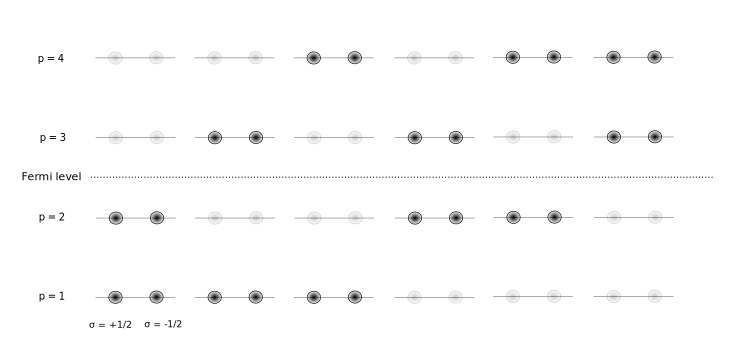
\includegraphics[width=1.1\linewidth]{Figures/Pairing_model2.pdf}
			\label{PairingModel_2}
			\caption{Configuration space for given pairing model showing all possible distributions of electrons}
		\end{figure}

	 	We need to diagonalize the Hamiltonian matrix, which is set up by calculating all the expectation values of all combination of states. The matrix elements will be set up as
		\begin{align}
			\begin{pmatrix}
				& \left| \Phi_0 \right> & \left| \Phi_{12}^{56} \right> & \left| \Phi_{12}^{78} \right> & \left| \Phi_{34}^{56} \right> & \left| \Phi_{34}^{78} \right> & \left| \Phi_{1234}^{5678} \right> \\ 
				\left< \Phi_0 \right| &   &   &   &   &   & \\
				\left< \Phi_{12}^{56} \right| &   &   &   &   &   & \\
				\left< \Phi_{12}^{78} \right| &   &   &   &   &   & \\
				\left< \Phi_{34}^{56} \right| &   &   &   &   &   & \\
				\left< \Phi_{34}^{78} \right| &   &   &   &   &   & \\
				\left< \Phi_{1234}^{5678} \right| &   &   &   &   &   & 
			\end{pmatrix}.
		\end{align}
		Excluding the 4p-4h excitations one does not diagonalize the exact matrix, but rather the approximated matrix known from Configuration Interaction. 
		The diagonal elements are calculated using Wick's theorem. Looking first at the ground state calculation with the unperturbed Hamiltonian part
		\begin{align}
			\left< \Phi_0 \right| \hat{\mathbf{H_0}} \left| \Phi_0 \right>,
		\end{align}
		we rewrite the states with respect to the vacuum state, we get the first equation for $\hat H_0$
		\begin{align}
			= \left< \right|  a_{2 \downarrow}  a_{2 \uparrow} a_{1 \downarrow} a_{1 \uparrow} \sum_{p \sigma} \delta (p-1) a_{p \sigma}^{\dagger} a_{p \sigma} 
			a_{1 \uparrow}^{\dagger} a_{1 \downarrow}^{\dagger} a_{2 \uparrow}^{\dagger} a_{2 \downarrow}^{\dagger} \left| \right>.
		\end{align}
		This expectation value can be contracted in four different ways, giving the final result 
		\begin{align}
			= 2 \delta (1-1) + 2 \delta (2-1) = 2 \delta.
		\end{align}
		The perturbation part, given by the expectation value 
		\begin{align}
			\left< \Phi_0 \right| \hat{\mathbf{V}} \left| \Phi_0 \right>,
		\end{align}
		written in terms of the vacuum state, this becomes 
		\begin{align}
			\left< \right| a_{2 \downarrow}  a_{2 \uparrow} a_{1 \downarrow} a_{1 \uparrow} \left( -g / 2 \sum_{pq} a_{p \uparrow}^{\dagger} a_{q \downarrow}^{\dagger} a_{q \downarrow} a_{p \uparrow} \right) 
			a_{1 \uparrow}^{\dagger} a_{1 \downarrow}^{\dagger} a_{2 \uparrow}^{\dagger} a_{2 \downarrow}^{\dagger} \left| \right>.
		\end{align}
		There are two ways this can contract, each contributing with the constant factor, $-g / 2$. 
		Performing similar calculations for all possible expectation values, will result in the final Hamiltonian matrix 
		\begin{align}
			\hat{\mathcal{H}} = \left( \begin{matrix}
				2 \delta - g & -g / 2 & -g / 2 & -g / 2 & -g / 2 & 0  \\
				-g / 2 & 4 \delta - g & -g / 2 & -g / 2 & 0 & -g / 2  \\
				-g / 2 & -g / 2 & 6 \delta - g & 0 & -g / 2 & -g / 2 \\
				-g / 2 & -g / 2 & 0 & 6 \delta - g & -g / 2 & -g / 2 \\
				-g / 2 & 0 & -g / 2 & -g / 2 & 8 \delta - g & -g / 2 \\
				0 & -g / 2 & -g / 2 & -g / 2 & -g / 2 & 10 \delta - g 
			\end{matrix} \right).
		\end{align}
		Diagonalizing this, and finding the smallest eigenvalue, will produce the exact energy for the Pairing model. 

	\end{section}

	\begin{section}{Hartree-Fock calculations}
		When doing Hartree-Fock calculations on the pairing model, the goal is to minimize the Hamiltonian expectation value through a change in basis. The ground state energy is given by 
		\begin{align}
			\left< \Phi_0 \right| \hat H \left| \Phi_0 \right> = E^{\text{HF}}.
		\end{align}
		This leads to the iterative equation 
		\begin{align}
  			\sum_{\gamma} h_{\alpha \gamma}^{\text{HF}} C_{a \gamma} = \epsilon_{a} C_{a \alpha},
  		\end{align}
  		where 
  		\begin{align}
  			h_{\alpha \gamma}^{\text{HF}} = \left< \alpha \right| h \left| \gamma \right> + \sum_{b=1}^N \sum_{\beta \delta} C_{b \beta}^* C_{b \delta} \left< \alpha \beta \right| v \left| \gamma \delta \right> .
  		\end{align}
  		For the first iteration, we must make a guess on the factors, $C_{b \beta}^*$ and $C_{b \delta}$. A natural starting point is to set
  		\begin{align}
  			C_{b \beta} = \delta_{b \beta} \:\:\:\:\:\: C_{b \delta} = \delta_{b \delta}.
  		\end{align}
  		This is the same as using the original basis in the first iteration, as there is no overlap between the states
  		\begin{align}
  			\left| \psi_a \right> = \sum_ \lambda \delta_{a \lambda} \left| \psi_ \lambda \right> .
  		\end{align}
  		To evaluate the Hartree-Fock matrix elements, we look at the states below Fermi level 
  		\begin{align}
  			\{p, \sigma\} \in \{ 1 \uparrow, 1 \downarrow, 2 \uparrow, 2 \downarrow \}.
  		\end{align}
  		The greek basis will therefore loop over these four states. The one-electron operator $\hat H_0$ is diagonal, so the matrix element
  		\begin{align}
  			\left< \alpha | h | \gamma \right> ,
  		\end{align}
 		will also be diagonal. Because of the starting point for the basis coefficients, we see that the two-electron operator can be written as
 		\begin{align}
 			V = \sum_{ b = 1 }^4 \left< \alpha b | v | \gamma b \right> .
 		\end{align}
 		Because the pairing model does not allow broken pairs, this matrix element will only be non-zero when $\alpha = \gamma$ and when $p_{\alpha} = p_{b}$, $\sigma_ \alpha = \sigma_b$. The Hartree-Fock matrix will therefore be diagonal, meaning the original basis is a canonical Hartree-Fock basis. Hartree-Fock calculations on this basis will not provide any new results. The Hartree-Fock energy can be calculated
 		\begin{align}
 			E^{\text{HF}} = \left< \Phi_0 \right| \hat H \left| \Phi_0 \right> = \left< \Phi_0 \right| \hat H_0 \left| \Phi_0 \right> + \left< \Phi_0 \right| \hat V \left| \Phi_0 \right>, 
 		\end{align}
 		which gives the result
 		\begin{align}
 			E^{\text{HF}} = 2 - g 
 		\end{align}
 		This energy will be referred to as the reference energy. 
 	\end{section}

	\begin{section}{Many-Body Perturbation Theory}
 		When setting up the many-body perturbation theory
                equations, it is useful to present them as
                diagrams. All the diagrams from   second to fourth
                order in perturbation theory are presented and translated
                to equations in this section.
 		
		Because of the properties of the pairing model, many
                of these diagrams can be removed by 
                examination. First, we have no broken pairs, meaning
                that a general two-body matrix element
		\begin{align}
			\left< pq | v | rs \right>,
		\end{align}
		is only non-zero if \textit{both} $p$ and $q$ are hole
                states or \textit{both} are particle states. The same
                restriction applies to $r$ and $s$. The second thing
                to notice, is that we have a canonical
                Hartree-Fock basis. That means only diagonal one-body matrix
                elements are non-zero. We will compute the correlation
                energy $\Delta E$, using the Hamiltonian
		\begin{align}
			\hat H_N = \hat F_N^d + \hat F_N^o + \hat W = \hat F_N^d + \hat W,
		\end{align}
		where
		\begin{align}
			f_{pq} = \epsilon_p \delta_{pq}.
		\end{align}
		The diagrams to second and third order, are presented in the following diagram
 		\begin{figure}[H]
			\includegraphics[width=\textwidth]{Figures/FirstSecondThirdOrder.pdf}
			\caption{Diagrams for Many-Body Perturbation theory to second and third order. }
			\label{figure:mbpt23}
		\end{figure}

		\begin{subsection}{Interpreting diagrams}
			When reading the diagrams, and connecting them to the equations presented in the equations (\ref{MBPT equations}), there are a simple set of rules. We have the expression for the resolvent, $\hat R_0$ given as 
			\begin{align}
				\hat R_0 = \frac{\hat Q}{E_0^{(0)} - \hat H_0} = \sum_I \frac{\left| \Phi_I \right> \left< \Phi_I \right| }{E_0^{(0)} - E_I^{(0)}},
			\end{align}
			where we sum over all states apart from $\left| \Phi_0 \right>$. When this operator operates on any state $\left| J \right>$ other than $\left| \Phi_0 \right> $, it will only produce, as shown in \cite{ShavittAndBartlett}, 
			\begin{align}
				\hat R_0 \left| J \right> = \left| J \right> \frac{1}{E_0^{(0)} - E_J^{(0)}}, 
			\end{align}
			meaning that the resolvent will only introduce a denominator expressed in terms of zeroth-order energies. We will introduce a more practical notation for this denominator
			\begin{align}
				\epsilon_{ij..}^{ab..} = E_0^{(0)} - E_{\left| \Phi_{ij..}^{ab..} \right> } = \epsilon_i + \epsilon_j + ... - \epsilon_a - \epsilon_b - ... .
			\end{align}
			The operator $\hat V$, as shown in equations (\ref{MBPT equations}), will give rise to matrix elements. If we have a canonical Hartree-Fock basis, we can rewrite the operator by 
			\begin{align}
				\hat V = \hat W + \hat F^o = \hat W ,
			\end{align}
			and there will only be two-body matrix elements present. Thich implies that all diagrams with one-body interactions can be removed. In the noncanonical Hartree-Fock case, $\hat F^o$ will give non-zero results and must be present. The procedure for interpreting the diagram and write out the corresponding equations can be summed up in the following sequence of operations
		\end{subsection}

		\begin{subsection}{Label all lines}
			First one should identify which lines represent hole states and which represent particle states, and label the lines with the corresponding letter, using $i,j,k,l,...$ for hole states and $a,b,c,d,...$ for particle states. 
		\end{subsection}

		\begin{subsection}{Identify the operators}
			A one-body vertex should be identified as the one-body operator used for the system, where one sets up the matrix element $f_p^q$ by the labels as
			\begin{align}
				f_p^q = \left< \text{line out} \right| \hat f \left| \text{line in} \right>.
			\end{align}
			The two-body vertices are identified as the two-body operators, and when identified, one should set up the corresponding matrix elements following the interpretation rule
			\begin{align}
				\left< pq || rs \right> = \left< \text{left in, right in} || \text{left out, right out} \right> .
			\end{align}
		\end{subsection}

		\begin{subsection}{Identify the denominator}
			To identify the denominator produced by the resolvent, $\hat R_0$, one draws imaginary lines between the interactions and set up the $\epsilon$ for every state-line that was crossed.
		\end{subsection}

		\begin{subsection}{Including phase factor}
			The resulting diagram will get a phase factor depending on how many hole states and how many closed loops there are. The factor is given by 
			\begin{align}
				(-1)^{\text{Closed loops} + \text{Number of holes}}.
			\end{align}
		\end{subsection}

		\begin{subsection}{Identify equivalent lines}
			Equivalent lines are pairs of lines that connect at the same vertices. They must also be of the same kind, either both particle states or both hole states. They will introduce a factor given as 
			\begin{align}
				\left( \frac{1}{2} \right)^{\text{number of equivalent lines}}.
			\end{align}
		\end{subsection}

		\begin{subsection}{Second Order Perturbation Theory}
			Starting with diagram 1, we see that this diagram is non-zero, because there is no one-body operator and no pairs are broken. We can set up the equation as
			\begin{align}
				E_\text{Diagram 1} = (-1)^{2+2} \frac{1}{2^2} \sum_{\substack{ab \\ ij}} \frac{\left< ij || ab \right> \left< ab || ij \right>}{\epsilon_{ij}^{ab}}.
			\end{align}
			Diagram 2 can be written out as
			\begin{align}
				E_\text{Diagram 2} = \sum_{ia} \frac{\left<i\right|f\left|a\right> \left<a\right| \hat f \left| i \right>}{\epsilon_i^a} = 0.
			\end{align}
			This diagram, however, will be zero. This is because we are operating with a canonical Hartree-Fock basis. By the definition of a non canonical Hartree Fock basis, $f_i^a = 0$, that basis would provide the same result. That means, only diagram 1 will provide a non-zero result for second order perturbation theory. 

		\end{subsection}

		\begin{subsection}{Third Order Perturbation Theory}
			The third order diagrams, shown in figure
                        \ref{figure:mbpt23}, are numbered from 3 to
                        15. Third order diagrams have three
                        interaction parts: One at the top and one at
                        the bottom of the diagram along with an
                        intermediate interaction part in the
                        middle. Applying the same logic that we
                        applied for diagram 2, we can exclude all
                        diagrams with a one-body interaction term,
                        leaving only diagrams 3, 4 and 5.
			\begin{align}
				E_{\text{diagram 3}} = \sum_{\substack{abc \\ ijk}} \frac{\left<ij||ab\right>\left<bk||jc\right>\left<ac||ij\right>}{\epsilon_{ij}^{ac} \epsilon_{ij}^{ab}} = 0. 
			\end{align}
			However, here we see a problem. We have an interaction term $\left<bk||jc\right>$, which is a broken pair. The Pairing model does not allow such states, and this must be zero. This is not a problem for the diagrams 4 and 5. 
			\begin{align}
				E_{\text{diagram 4}} = \frac{1}{2^3} \sum_{\substack{abcd \\ ij}} \frac{\left<cd||ij\right>\left<ab||cd\right>\left<ij||ab\right>}{\epsilon_{ij}^{cd} \epsilon_{ij}^{ab}},
			\end{align}
			\begin{align}
				E_{\text{diagram 4}} = \frac{1}{2^3} \sum_{\substack{ab \\ ijkl}} \frac{\left<ab||kl\right>\left<kl||ij\right>\left<ij||ab\right>}{\epsilon_{kl}^{ab} \epsilon_{ij}^{ab}}.
			\end{align}
			When doing many-body perturbation theory to
                        third order with a canonical Hartree-Fock
                        basis for the pairing model, one only needs
                        to calculate diagrams 1, 4 and 5.

		\end{subsection}

		\begin{subsection}{Fourth Order Perturbation Theory}
			When calculating the correlation energy with the fourth order energy, the second and third order are included as well. The amount of diagrams increase dramatically when adding the fourth order, but as we only work with a canonical Hartree-Fock basis, the amount is somewhat limited \cite{ShavittAndBartlett}. We group the diagrams by the excitations they produce, i.e. how many pairs of external lines that are present.. 
			\begin{figure}[H]
				\includegraphics[width=\textwidth]{Figures/fourthorder1p1h.png}
				\caption{Goldstone diagrams for fourth order Rayleigh-Schr\"{o}dinger perturbation theory with 1p1h excitations}
				\label{figure:mbpt1p1h}
			\end{figure}
			The first set of diagrams in figure (\ref{figure:mbpt1p1h}) show diagrams giving rise to a 1particle-1hole excitation. All these diagrams have an intermediate step with a 1p-1h part. The Pairing model does not allow broken pairs, meaning that intermediate steps with 1p-1h or 3p-3h interaction parts must be zero. Therefore none of these diagrams are included in the calculations.
			\begin{figure}[H]
				\includegraphics[width=\textwidth]{Figures/fourthorder2p2h.png}
				\caption{Goldstone diagrams for fourth order Rayleigh-Schr\"{o}dinger perturbation theory with 2p2h excitations}
				\label{figure:mbpt2p2h}
			\end{figure}
			The set of diagrams shown in figure (\ref{figure:mbpt2p2h}), give rise to a 2 particle and 2 hole excitation. For all these diagrams, there are only 2p-2h interaction parts for all intermediate steps. However, many of these diagrams give rise to a broken pair interaction of the form 
			\begin{align}
			 	\left< ai || pq \right> .
			\end{align}
			Only the diagrams 5,6,14 and 15 have no broken pair interactions. They are calculated as
			\begin{align}
				E_{\text{diagram 5}} = \frac{1}{2^4} \sum_{\substack{abcd\\ijkl}} \frac{ \left<cd||kl\right>\left<kl||ij\right>\left<ab||cd\right>\left<ij||ab\right> }{ \epsilon_{kl}^{cd} \epsilon_{ij}^{cd} \epsilon_{ij}^{ab} },
			\end{align} 
			and diagram 6
			\begin{align}
				E_{\text{diagram 6}} = \frac{1}{2^4} \sum_{\substack{abcd\\ijkl}} \frac{ \left<cd||kl\right>\left<kl||ij\right>\left<ab||cd\right>\left<ij||ab\right> }{ \epsilon_{kl}^{ab} \epsilon_{kl}^{cd} \epsilon_{ij}^{ab} }.
			\end{align} 
			For diagram 14, we get 
			\begin{align}
				E_{\text{diagram 14}} = \frac{1}{2^4} \sum_{\substack{abcdef\\ij}} \frac{ \left<ij||ab\right>\left<ab||cd\right>\left<cd||ef\right>\left<ef||ij\right> }{ \epsilon_{ij}^{ab} \epsilon_{ij}^{cd} \epsilon_{ij}^{ef} },
			\end{align} 
			and for diagram 15
			\begin{align}
				E_{\text{diagram 15}} = \frac{1}{2^4} \sum_{\substack{ab\\ijklmn}} \frac{ \left<ij||ab\right>\left<kl||ij\right>\left<mn||kl\right>\left<ab||mn\right> }{ \epsilon_{ij}^{ab} \epsilon_{kl}^{ab} \epsilon_{mn}^{ab} }
			\end{align} 

			\begin{figure}[H]
				\includegraphics[width=\textwidth]{Figures/fourthorder3p3h.png}
				\caption{Goldstone diagrams for fourth order Rayleigh-Schr\"{o}dinger perturbation theory with 3p3h excitations}
				\label{figure:mbpt3p3h}
			\end{figure}
			The diagrams depicted in figure (\ref{figure:mbpt3p3h}), show the fourth order diagrams giving rise to 3 particles and 3 holes excitations. We notice that all these diagrams include one intermediate step with a 3p-3h excitation. Therefore we can exclude all these diagrams from the calculations.  

			\begin{figure}[H]
				\includegraphics[width=\textwidth]{Figures/fourthorder4p4h.png}
				\caption{Goldstone diagrams for fourth order Rayleigh-Schr\"{o}dinger perturbation theory with 4p4h excitations}
				\label{figure:mbpt4p4h}
			\end{figure}
			The last set of diagrams, depicted in figure (\ref{figure:mbpt4p4h}), show the fourth order diagrams that include a 4 particle and 4 hole part. Invoking the Linked diagram theorem, we can immediatly exclude diagram 33 and diagram 41. Diagram 34 to 40 do will be non-zero, and must be calculated. For diagram 34, we get
			\begin{align}
				E_{\text{diagram 34}} = \left(-1\right)^{(3+4)} \frac{1}{2^2} \sum_{\substack{abcd\\ijkl}} \frac{ \left<ij||ab\right>\left<kl||cd\right>\left<ab||ik\right>\left<cd||jl\right> }{ \epsilon_{ij}^{ab} \epsilon_{ijkl}^{abcd} \epsilon_{jl}^{cd} }.
			\end{align}
			We notice that there are 3 closed loops and 4 hole states, giving rise to the negative phase factor. We also notice that we have two pairs of equivalent lines, arising from the particle states, introducing a factor $\frac{1}{4}$. One can also notice the fourth order denominator term $\epsilon_{ijkl}^{abcd}$, arising from the 4p-4h intermediate excitation part. The last diagrams are calculated following the same principles, giving 
			\begin{align}
				E_{\text{diagram 35}} = \left(-1\right)^{(3+4)} \frac{1}{2^2} \sum_{\substack{abcd\\ijkl}} \frac{ \left<ij||ab\right>\left<kl||cd\right>\left<ac||ij\right>\left<bd||kl\right> }{ \epsilon_{ij}^{ab} \epsilon_{ijkl}^{abcd} \epsilon_{kl}^{bd} },
			\end{align}
			Before calculating diagram 36, please notice that there is a mistake in the drawing of the diagram 36. The right-most particle state is supposed to be a hole state, giving the correct equation 
			\begin{align}
				E_{\text{diagram 36}} = \frac{1}{2^4} \sum_{\substack{abcd\\ijkl}} \frac{ \left<ij||ab\right>\left<kl||cd\right>\left<ab||kl\right>\left<cd||ij\right> }{ \epsilon_{ij}^{ab} \epsilon_{ijkl}^{abcd} \epsilon_{ij}^{cd} }.
			\end{align}
			Diagram 37 is also depicted with the right-most state wrong. It is supposed to be a particle state, giving
			\begin{align}
				E_{\text{diagram 37}} = \frac{1}{2^4} \sum_{\substack{abcd\\ijkl}} \frac{ \left<ij||ab\right>\left<kl||cd\right>\left<cd||ij\right>\left<ab||kl\right> }{ \epsilon_{ij}^{ab} \epsilon_{ijkl}^{abcd} \epsilon_{kl}^{ab} }.
			\end{align}
			and for diagram 38, we notice that there are no equal state pairs
			\begin{align}
				E_{\text{diagram 38}} = \sum_{\substack{abcd\\ijkl}} \frac{ \left<ij||ab\right>\left<kl||cd\right>\left<db||lj\right>\left<ac||ik\right> }{ \epsilon_{ij}^{ab} \epsilon_{ijkl}^{abcd} \epsilon_{ik}^{ac} }.
			\end{align}
			Diagram 39 gives
			\begin{align}
				E_{\text{diagram 39}} = \left(-1\right)^{(3+4)} \frac{1}{2^2} \sum_{\substack{abcd\\ijkl}} \frac{ \left<ij||ab\right>\left<kl||cd\right>\left<bd||kl\right>\left<ac||ij\right> }{ \epsilon_{ij}^{ab} \epsilon_{ijkl}^{abcd} \epsilon_{ij}^{ac} }.
			\end{align}
			And finally, diagram 40 gives the equation
			\begin{align}
				E_{\text{diagram 40}} = \left(-1\right)^{(3+4)} \frac{1}{2^2} \sum_{\substack{abcd\\ijkl}} \frac{ \left<ij||ab\right>\left<kl||cd\right>\left<cd||jl\right>\left<ab||ik\right> }{ \epsilon_{ij}^{ab} \epsilon_{ijkl}^{abcd} \epsilon_{ik}^{ab} }.
			\end{align}
		\end{subsection}
 		
 	\end{section}

 	\begin{section}{Spin Summations}
 		Up to this point, we have not taken into account the effect of spin in the matrix elements. Because of spin orthogonality, terms may vanish from certain two-electron matrix elements. Listed here, are all the different ways spins can be organized, along with the resulting integration. Representing the spin up orbital with a bar, we get \cite{ShavittAndBartlett}
 		\begin{align}
 			\left< pq || rs \right> &= \left< pq | \hat v | rs \right> - \left< pq | \hat v | sr \right>, \\
 			\left< p\bar q || r\bar s \right> &= \left<pq | \hat v | rs \right> ,\\
 			\left< p \bar q|| \bar r s \right> &= - \left<pq | \hat v | sr \right> ,\\
 			\left< \bar p q|| \bar r s\right> &= \left< pq | \hat v | rs \right>, \\
 			\left< \bar p q|| r \bar s \right> &= - \left< pq | \hat v | sr \right>, \\
 			\left< \bar p \bar q || \bar r \bar s \right> &= \left< pq | \hat v | rs \right> - \left< pq | \hat v | sr \right> .
 		\end{align}
 		Because of the restrictions on the pairing model, the first and the last equations will also be zero, because the states are not allowed to exist. Matrix elements, where there are an unequal amount of equal spin orbitals will all give zero as result as well
 		\begin{align}
 			\left< \bar p q || rs \right> &= \left< p \bar q || rs \right> = \left< pq || \bar r s \right> = \left< pq || r \bar s \right> = 0, \\
 			\left< \bar p \bar q || rs \right> &= \left< pq || \bar r \bar s \right>  = 0 ,\\
 			\left< \bar p \bar q || \bar r s \right> &= \left< \bar p \bar q || r \bar s \right> = \left< \bar p q || \bar r \bar s \right> = \left< p \bar q || \bar r \bar s \right> = 0.
 		\end{align} 


 	\end{section}

\end{chapter}



\begin{chapter}{Infinite Matter}
	A study of infinite matter can convey important information about the equation of state in dense objects like neutron stars, and hopefully shed light on the strong force acting in a many-body medium. This thesis will study the infinite electron gas before the final study of nuclear matter. This is done for pedagogical reasons and because the electron gas has closed form solutions that provide important benchmarking for the code. 
	\begin{section}{The Infinite Electron Gas}
		The infinite electron gas gives a good approximation to valence electrons in metal. The gas consists only of interacting electrons with a uniform background of charged ions. The whole system is charge neutral. We assume a finite cubic box as done in \cite{Shepherd2012} and \cite{Shepherd2013}. The box has a length $L$ and volume $\Omega = L^3$, with $N_e$ as the number of electrons with a charge density $\rho = N_e / \Omega$.

		\begin{subsection}{The Hamiltonian}
			The electrons interact with the central symmetric Colomb potential, $\hat V(\vec r_1, \vec r_2)$ depending only on the distance $\left| \vec r_1 - \vec r_2 \right|$. The Hamiltonian for infinite electron gas is \cite{Baardsen}
			\begin{align}
				\hat H = \hat H_1 + \hat H_2 = \hat H_{\text{kin}} + \hat H_{\text{interaction}}.
			\end{align}
			The interaction term will be dependent on both the electron-electron interaction, the electron-background interaction and the background-background interaction
			\begin{align}
				\hat H = \hat H_{\text{kin}} + \hat H_{\text{ee}} + \hat H_{\text{eb}} + \hat H_{\text{bb}}.
			\end{align}
			The kinetic energy, $\hat H_{\text{kin}}$ is given as
			\begin{align}
				\hat H_{\text{kin}} = \sum_p \frac{\hbar ^2 k^2}{2m} a_{k \sigma}^{\dagger} a_{k \sigma}.
			\end{align}
			The background-interaction terms will vanish as explained by Fraser et al \cite{Fraser et al} both for three- and two-dimensional electron gas. When we sum over all particles, we can write the electron-electron interaction term as an Ewald summation term, because it is not possible to use a $1/r$ term for infinite systems \cite{Drummond2008} \cite{MHJonline}. We can write this term as
			\begin{align}
				\hat H_{ee} = \sum_{i<j}^N v_E(\mathbf{r}_i - \mathbf{r}_j) + \frac{1}{2}Ne^2v_0,
			\end{align}
			where $v_E(\mathbf{r})$ is an effective two-body interaction. $v_0$ is the self-interaction term, defined as 
			\begin{align}
				v_0 = \lim_{\mathbf{r}\rightarrow \infty} \left\{ v_E(\mathbf{r}) - \frac{1}{r} \right\}.
			\end{align}
			The Ewald summation will account for interactions between all electrons in the finite size system as well as all the image electrons that will arize from self-interaction because of periodic boundaries. We define it as 
			\begin{align}
				v_E(\mathbf{r}) &= \sum_{k \neq 0} \frac{4\pi}{L^3k^2} e^{i \mathbf{k}\cdot \mathbf{r} } e^{-\eta^2 k^2 / 4} \\
								&+ \sum_{\mathbf{R}} \frac{1}{|	\mathbf{r} - \mathbf{R}|} \text{erfc} \left( \frac{| \mathbf{r} - \mathbf{R}|}{\eta} \right) - \frac{\pi \eta^2}{L^3}, \nonumber
			\end{align}
			where $L$ is the size of the box, $\mathbf{k}$ is the momentum vector, while $\mathbf{r}$ represent the position vectors for all electrons. The translational vector $\mathbf{R}$, is used to obtain all image cells in the entire real space \cite{MHJonline}
			\begin{align}
				\mathbf{R} = L(n_x \mathbf{u}_x + n_y \mathbf{u}_y + n_z \mathbf{u}_z).
			\end{align}
			We have used the error functions
			\begin{align}
				\text{erf}(x) = \frac{2}{\sqrt{\pi}} \int_0^x e^{-t^2} \text{dt},
			\end{align}
			and
			\begin{align}
				\text{erfc}(x) = 1 - \text{erf}(x) = \frac{2}{\sqrt{\pi}} \int_x^\infty e^{-t^2} \text{dt}.
			\end{align}
			We use this relation because an interaction on the form $1/|r|$ is not convergent for an infinite number of particles \cite{Audun}. Ewald found that one can rewrite the interaction in terms of these error functions \cite{Ewald}
			\begin{align}
				\frac{1}{r} = \frac{\text{erf}(\frac{1}{2}\sqrt{\eta}r)}{r} + \frac{\text{erfc}(\frac{1}{2}\sqrt{\eta}r)}{r}.
			\end{align}
			One can calculate the two-dimensional Ewald term as well \cite{Baardsen}, resulting in 
			\begin{align}
				v_E^{\eta=0, z=0} = \sum_{\mathbf{k} \neq 0} \frac{2 \pi}{L^2 k} e^{i \mathbf{k} \cdot \mathbf{r}_{xy}}.
			\end{align}
		\end{subsection}
		
		\begin{subsection}{The Reference Energy}
			The reference energy for electron gas can be written as \cite{Baardsen}
			\begin{align}
				E_{\text{ref}} = \sum_i \left<i | h_0 | i\right> + \frac{1}{2} \sum_{ij} \left<ij||ij\right> + \frac{1}{2} Av_0.
			\end{align}
			$A$ is the number of electrons, and the term $A v_0$ is the so-called Madelung constant. It is how we incorporate the self-interaction term into the system. This factor will be larger for smaller system and vanish as we approach the thermodynamic limit. 
		\end{subsection}
		
		\begin{subsection}{The Fock Matrix Elements}
			The Fock Matrix Elements will be given as
			\begin{align}
				\left< p | f | q \right> = \frac{k_p^2}{2m} \delta_{\mathbf{k}_p \mathbf{k}_q} \delta_{m_{s_p} m_{s_q}} + \sum_i \left<pi||qi\right>.
			\end{align}
			We notice that the Fock Matrix elements can be written as a diagonal part plus the $\hat U$ operator. As we can see from (\ref{3.93}) and (\ref{3.95}), this means the perturbation is given solely by the two-body interaction
			\begin{align}
				\hat V = \frac{1}{4} \sum_{pqrs} \left<pq||rs\right> \hat p^\dagger \hat q^\dagger \hat s \hat r.
			\end{align}
		\end{subsection}

		\begin{subsection}{Anti-Symmetric Matrix Elements}
			We now need to define the matrix elements for the two- and three-dimensional electron gas to calculate the perturbation 
			\begin{align}
				&\left< \mathbf{k}_p m_{s_p} \mathbf{k}_q m_{s_q} || \mathbf{k}_r m_{s_r} \mathbf{k}_s m_{s_s} \right> \\
				&= \frac{4 \pi e^2}{L^3} \delta_{\mathbf{k}_p + \mathbf{k}_q, \mathbf{k}_r + \mathbf{k}_s} \left\{ \delta_{ m_{s_p},m_{s_r} } \delta_{ m_{s_q},m_{s_s} } (1 - \delta_{\mathbf{k}_p, \mathbf{k}_r}) \frac{1}{| \mathbf{k}_r - \mathbf{k}_p|^2} \right. \nonumber \\
				& - \delta_{ m_{s_p},m_{s_s} } \delta_{ m_{s_q},m_{s_r} } (1 - \delta_{\mathbf{k}_p, \mathbf{k}_s}) \left. \frac{1}{| \mathbf{k}_s - \mathbf{k}_p|^2}  \right\}. \nonumber
			\end{align}
			The two-dimensial case is almost identical
			\begin{align}
				&\left< \mathbf{k}_p m_{s_p} \mathbf{k}_q m_{s_q} || \mathbf{k}_r m_{s_r} \mathbf{k}_s m_{s_s} \right> \\
				&= \frac{2 \pi e^2}{L^2} \delta_{\mathbf{k}_p + \mathbf{k}_q, \mathbf{k}_r + \mathbf{k}_s} \left\{ \delta_{ m_{s_p},m_{s_r} } \delta_{ m_{s_q},m_{s_s} } (1 - \delta_{\mathbf{k}_p, \mathbf{k}_r}) \frac{1}{| \mathbf{k}_r - \mathbf{k}_p|} \right. \nonumber \\
				& - \delta_{ m_{s_p},m_{s_s} } \delta_{ m_{s_q},m_{s_r} } (1 - \delta_{\mathbf{k}_p, \mathbf{k}_s}) \left. \frac{1}{| \mathbf{k}_s - \mathbf{k}_p|}  \right\}. \nonumber
			\end{align}		
		\end{subsection}

		\begin{subsection}{The Plane Wave Basis}
			When set up with periodic boundary conditions, the homogenous electron gas can be set up with free particle normalized wave functions
			\begin{align}
				\psi_{\vec k \sigma} (\vec r) = \frac{1}{\sqrt{\Omega}} e^{i \vec k \vec r} \xi_{\sigma},
			\end{align}
			where $\vec k$ is the wave number and $\xi_{\sigma}$ is a spin function. 
			\begin{align}
				\xi_{+\frac{1}{2}} = \left( \begin{matrix} 1 \\ 0 \end{matrix} \right), \:\;\:\; \xi_{-\frac{1}{2}} = \left( \begin{matrix} 0 \\ 1 \end{matrix} \right).
			\end{align}
			Because of periodic boundary conditions, we acquire the following wave numbers
			\begin{align}
				k_i = \frac{2\pi n_i}{L}, \:\:\:\;\; i = x,y,z \;\;\:\:\: n_i = 0, \pm 1, \pm 2, ... .
			\end{align}
			and the associated single-particle energies for two dimensions
			\begin{align}
				\epsilon_{n_x,n_y} = \frac{\hbar^2}{2m} \left( \frac{2\pi}{L} \right)^2 (n_x^2 + n_y^2).
			\end{align}
			For three dimensions, we get the energy 
			\begin{align}
				\epsilon_{n_x,n_y,n_z} = \frac{\hbar^2}{2m} \left( \frac{2\pi}{L} \right)^2 (n_x^2 + n_y^2 + n_z^2 ).
			\end{align}
			By the nature of the single particle energies, the energy levels will be determined by the value of $n_x^2 + n_y^2 + n_z^2$. There are different combinations of $n_x, n_y$ and $n_z$ that set up each energy level. The cumulative number of particles needed to completely fill these energy states will be named \textit{magic numbers} and are listed in table \ref{Magic Numbers 3d}. 
			\begin{table}[H]
				\begin{center}
					\begin{tabular}[center]{l | c c c | c | c | r }
						$n_x^2 + n_y^2 + n_z^2$ & $n_x$ & $n_y$ & $n_z$ & $N_{\uparrow \uparrow}$ & $N_{\uparrow \downarrow}$ & $N_{\uparrow \downarrow} \hat \tau$ \\
						\hline
						0 & 0 & 0 & 0 & 1 & 2 & 4 \\
						\hline
						1 & 1 & 0 & 0 &   &   &   \\
						  & -1& 0 & 0 &   &   &   \\
						  & 0 & 1 & 0 &   &   &   \\
						  & 0 & -1& 0 &   &   &   \\
						  & 0 & 0 & 1 &   &   &   \\
						  & 0 & 0 & -1& 7 & 14& 28\\
						\hline
						2 & 1 & 1 & 0 &   &   &   \\
						  & 1 & -1& 0 &   &   &   \\
						  & 1 & 0 & 1 &   &   &   \\
						  & 1 & 0 & -1&   &   &   \\
						  & -1& 1 & 0 &   &   &   \\
						  & -1& -1& 0 &   &   &   \\
						  & -1& 0 & 1 &   &   &   \\
						  & -1& 0 & -1&   &   &   \\
						  & 0 & 1 & 1 &   &   &   \\
						  & 0 & 1 & -1&   &   &   \\
						  & 0 & -1& 1 &   &   &   \\
						  & 0 & -1& -1&19 &38 & 76\\
						\hline
						3 & 1 & 1 & 1 &   &   &   \\
						  & 1 & 1 & -1&   &   &   \\
						  & 1 & -1& 1 &   &   &   \\
						  & 1 & -1& -1&   &   &   \\
						  & -1& 1 & 1 &   &   &   \\
						  & -1& 1 & -1&   &   &   \\
						  & -1& -1& 1 &   &   &   \\
						  & -1& -1& -1&27 & 54&108\\
						\hline
						4 & 2 & 0 & 0 &   &   &   \\
						  & -2& 0 & 0 &   &   &   \\
						  & 0 & 2 & 0 &   &   &   \\
						  & 0 & -2& 0 &   &   &   \\
						  & 0 & 0 & 2 &   &   &   \\
						  & 0 & 0 & -2& 33& 66&132\\
						\hline
						5 &   &   &   & 57&114&228\\
						\hline
						6 &   &   &   & 81&162&324\\
						\hline
						7 &   &   &   & 81&162&324\\
						\hline
						8 &   &   &   & 93&186&372
					\end{tabular}
				\end{center}
				\caption{All magic numbers for three dimensional infinite matter. The table demonstrates how states will fill up energy levels. $n_x$, $n_y$ and $n_z$ represent momentum quantum numbers, $n_x^2 + n_y^2 + n_z^2$ represent energy level. $N_{\uparrow \uparrow}$ shows magic number without spin degeneracy, $N_{\uparrow \downarrow}$ adds two possible spins, and $N_{\uparrow \downarrow} \hat \tau $ also adds isospin degeneracy.} 
				\label{Magic Numbers 3d}
			\end{table}

		\end{subsection}

	\end{section}

	\begin{section}{Infinite Nuclear Matter}
		Central to my thesis, is the study of infinite nuclear
                matter. I look at baryonic matter similar to the dense
                baryonic matter found in neutron stars. I limit the
                study to temperatures far below the Fermi level
                temperature, assuming thereby that I can treat
                neutrons and protons as a degenerate Fermi gas. The
                matter is mostly made up of neutron and protons in
                $\beta$-equilibrium with the relevant leptons. 
                The
                equilibrium conditions are specified by
		\begin{align}
		 	b_1 \rightarrow b_2 + l + \bar \nu_l \:\:\:\:\:\: b_2 + l \rightarrow b_1 + \nu_l,
		\end{align} 
		where $b$ represent either a neutron or a proton and $l$ is either an electron or muon. $\nu_l$ is the corresponding neutrino. 

		Nuclear matter is a hypothetical system filling all of
                space at a uniform density. Symmetric nuclear matter
                (SNM) consist of equal numbers of protons of neutrons,
                while pure nuclear matter (PNM) consist only of
                neutrons. For finite-nucleus systems, the most
                difficult part is calculating the single particle wave
                function. For nuclear matter we can use the same plane
                wave basis that we used for the electron gas. The
                difficult part is calculating the energy and the
                effective interaction between particles
                \cite{Day1967}. In my calculations, I have looked at
                pure neutron  matter only.
	\end{section}

	\begin{section}{Nuclear Interaction}
		Nuclear matter is composed of baryons which interact through the strong force. Here we will employ a simplified model of the nuclear forces, the so-called Minnesota potential. This potential has been widely used in studies of different many-body methods.
		
		\begin{subsection}{The Minnesota Potential}
			The Minnesota Potential is given as
			\begin{align}
				v(r) = &\left(v_R + (1 + P_{12}^\sigma) v_T/2 + (1 - P_{12}^\sigma) v_S/2 \right) \\
					   \cdot &\left( \alpha + (2- \alpha)P_{12}^r \right)/2 + (1+m_{t,1})(1+m_{t,2})\frac{e^2}{4r}, \nonumber
			\end{align}
			where $r$ is given as $\left| \mathbf{r_1} - \mathbf{r_2} \right|$ and $m_t$ is the isospin projection of particle 1 or 2. $m_t = \pm 1$. 
			$P_{12}^\sigma $ and $P_{12}^r$ are exchange operators for spin and position, respectively \cite{Baardsen}. Furthermore, we have used
			\begin{align} 
				v_R = v_{0R}e^{-k_R r^2}, \:\:\: v_T = -v_{0T} e^{-k_Tr^2}, \:\:\: v_S = -v_{0S}e^{-k_sr^2},
			\end{align}
			where the constants $v_{0R}$, $v_{0T}$, $v_{0S}$, $k_R$, $k_T$ and $k_S$ are given by \cite{Thompson1977}
			\begin{enumerate}
				\item $v_{0R} = 200$MeV,  $k_R = 1.487 \text{fm}^{-2}$,
				\item $v_{0T} = 178$MeV,  $k_T = 0.649 \text{fm}^{-2}$,
				\item $v_{0S} = 91.85$MeV, $k_S = 0.465 \text{fm}^{-2}$.
			\end{enumerate}
In momentum space the interaction reads
			\begin{align}
			 	\left<k_p k_q \middle| v \middle| k_r k_s \right> = \frac{V_0}{L^3} \left(\frac{\pi}{\alpha}\right)^{3/2} e^{-q^2 / 4 \alpha} \delta_{\vec k_p + \vec k_q, \vec k_r + \vec k_s},
			\end{align}
			where $q$ is the relative momentum transfer given by 
			\begin{align}
				\mathbf{q} = \mathbf{p} - \mathbf{p'},
			\end{align}
			and the momentum vectors are defined as
			\begin{align}
				\mathbf{p} = \frac{1}{2} (\mathbf{k}_p - \mathbf{k}_q), \:\:\:\:\: \mathbf{p'} = \frac{1}{2}(\mathbf{k}_r- \mathbf{k}_s).
			\end{align}
			We can now set up the two-body Matrix-elements for the Minnesota Potential
			\begin{align}
				\left<\mathbf{k}_p \mathbf{k}_q \middle| v \middle| \mathbf{k}_r \mathbf{k}_s \right> = 
				&\left<\mathbf{k}_p \mathbf{k}_q \right| \frac{1}{2} \left( V_R + \frac{1}{2} V_T + \frac{1}{2} V_S \right) \left| \mathbf{k}_r \mathbf{k}_s \right>   \\
				+&\left<\mathbf{k}_p \mathbf{k}_q \right| \frac{1}{4} (V_T - V_S) P_{12}^\sigma \left| \mathbf{k}_r \mathbf{k}_s \right> \nonumber \\
				-&\left<\mathbf{k}_p \mathbf{k}_q \right| \frac{1}{2} \left( V_R + \frac{1}{2} V_T + \frac{1}{2} V_S \right) P_{12}^\sigma P_{12}^\tau \left| \mathbf{k}_r \mathbf{k}_s \right> \nonumber \\
				-&\left<\mathbf{k}_p \mathbf{k}_q \right| \frac{1}{4}(V_T - V_S) P_{12}^\tau  \left| \mathbf{k}_r \mathbf{k}_s \right>&. \nonumber
			\end{align}
			Matrix elements for the spin and isospin exchange operators are 
			\begin{align}
				\left< \sigma_p \sigma_q \right| P_{12}^\sigma \left| \sigma_r \sigma_s \right> = \delta_{\sigma_p,\sigma_s} \delta_{\sigma_q,\sigma_r}.
			\end{align}
			One can see that these matrix elements come at
                        a far greater computational cost than the
                        electron-electron interaction in the electron
                        gas. Therefore, storing the matrix elements instead of computing them
                        "on the fly" can lead to a significant boost in performance \cite{MHJonline}.
		\end{subsection}
		
	\end{section}

\end{chapter}



\begin{chapter}{Implementation of CCD}
	In this thesis I have created three different solvers for coupled-cluster doubles equations. 
	\begin{enumerate}
		\item A naive brute force implementation of the equations summing over all variables. 
		\item A naive brute force implementation of intermediate equations summing over all variables.
		\item Rewriting the summations as matrix-matrix multiplications and exploiting various symmetry arguments that one can set up as a block implementation.
	\end{enumerate}	
	There is a significant performance leap between each method,
        but I have included the first two solvers for both educational
        and benchmarking purposes. The pairing model with 4 particles
        and 4 holes is a small system that one can easily solve using
        the naive approach. After producing expected results with the
        naive solver, I have compared the more complicated solvers to
        the naive solver for all systems.

	\begin{section}{Implementing the CCD equations}
		The basic steps of all implemented CCD algorithms can
                be explained through the following four steps:
		\begin{enumerate}
			\item Initialize amplitudes $t^{(0)} = 0$ and $\Delta E_{CCD}^{(0)} = 0$.
			\item Update the amplitudes and calculate $\Delta E_{CCD}^{(1)}$.
			\item If $ |\Delta E_{CCD}^{(1)} - \Delta E_{CCD}^{(0)}| \geq \epsilon $, update amplitudes and compute $\Delta E_{CCD}^{2}$.
			\item Repeat until $ |\Delta E_{CCD}^{(n+1)} - \Delta E_{CCD}^{(n)}| \leq \epsilon $.
		\end{enumerate}
		The difference between the three solvers I have
                implemented is the way I update amplitudes. The naive
                brute force solver loops over all indices when
                computing. An example of diagram $L_a$ is shown below

		\begin{lstlisting}
		for i in 0, ..., Nholes:
			for j in 0, ..., Nholes:
				for a in Nholes, ..., Nparticles:
					for b in Nholes, ..., Nparticles:
						for c in Nholes, ..., Nparticles:
							for d in Nholes, ..., Nparticles:
								tnew(a,b,i,j) = 0.5 * v(a,b,c,d) * told(c,d,i,j) / epsilon(i,j,a,b);
		\end{lstlisting}

		A significant cost reduction can be obtained by
                factorizing the diagrams as shown in equation
                (\ref{Intermediates}). By calculating the four
                intermediate diagrams, $I_1$, $I_2$, $I_3$ and $I_4$
                beforehand and storing the results reduce the cost of
                calculation from $\mathcal{O}(h^4 p^4)$ to
                $\mathcal{O}(h^4 p^2)$. The second solver applies this
                method.

                The solver might diverge when iterating, and a work-around for this, is to include a relaxing factor, $\alpha$ when updating the amplitudes. This can be implemented as
                \begin{align}
                  t_{\text{new}} = \alpha t_{\text{new}} + (1-\alpha) t_{\text{old}}
                \end{align}

	\end{section}

	\begin{section}{Matrix Representation of Contractions}
		Diagrams can be viewed as contractions of tensors of
                varying degree. An example is the matrix-matrix
                multiplication product
		\begin{align}
		 	\left( M N \right)_{\gamma}^{\alpha} = \sum_{\beta} M_{\beta}^\alpha N_\gamma^\beta .
		 	\label{matrix matrix multiplication}
		\end{align} 

		As our goal is to rewrite the coupled-cluster
                equations as matrix-matrix products, we will need to
                map tensors of rank $\geq 2$ onto matrices. One
                mapping that provides systematic and unique matrix
                elements is
		\begin{align}
			\left<pq\middle| \hat v\middle|rs\right> = V_{\alpha(p,q),\beta(r,s)},
		\end{align}
		where 
		\begin{align}
			\alpha(p,q) = p + q N_p, \;\,\:\; \beta(r,s) = r + s N_r.
			\label{mapping of matrix elements}
		\end{align}
		We need to be careful when mapping tensors this
                way. Consider first the calculation of the perfectly
                aligned $L_a$ term
		\begin{align}
			L_a = \sum_{cd} \left< ab \middle| \hat v\middle|cd\right> t_{ij}^{cd}.
		\end{align}
		Mapping this equation using equation (\ref{mapping of matrix elements})
		\begin{align}
			\left< ab \middle| \hat v\middle|cd\right> = v_{ab}^{cd} \rightarrow V_{\beta(c,d)}^{\alpha(a,b)},
		\end{align}
		and
		\begin{align}
			t_{ij}^{cd} \rightarrow T_{\delta(i,j)}^{\beta(c,d)}.
		\end{align}
		As we are mapping to unique elements 
		\begin{align}
			\beta(c,d) = \beta(c,d),
		\end{align}
		we can now rewrite the equation 
		\begin{align}
			(L_a)_ \delta^\alpha = \sum_ \beta V_ \beta^\alpha T_ \delta^\beta,
		\end{align}
		implying by regarding equation (\ref{matrix matrix multiplication}) that we can rewrite the product as a matrix-matrix multiplication 
		\begin{align}
			L_a = VT.
		\end{align}

		\begin{subsection}{Aligning elements}	
			Unfortunately, not all products are perfectly aligned like $L_a$. Consider, for example, the term $L_c$
			\begin{align}
				L_c = -P\left(ij\middle|ab\right) \sum_{kc} \left<kb\middle|\hat v\middle|cj\right>t_{ik}^{ac}.
			\end{align}
			Using the same mapping scheme
			\begin{align}
				\left<kb\middle|\hat v\middle|cj\right> = v_{cj}^{kb} \rightarrow V_{\beta(cj)}^{\alpha(kb)},
			\end{align}
			and
			\begin{align}
				t_{ik}^{ac} \rightarrow T_{\delta(ik)}^{\gamma(ac)},
			\end{align}
			we notice that this matrix multiplication is misaligned, and if the number of particles is unequal to the number of holes, the  size of the matrices will be incompatible
			\begin{align}
				(L_c)_ \delta^\alpha \neq -P\left(ij\middle|ab\right) \sum_ \beta V_{\beta(cj)}^{\alpha(kb)} T_{\delta(ik)}^{\gamma(ac)}.
			\end{align}
			We need to find another mapping, such as
			\begin{align}
				v_{cj}^{kb} \rightarrow \tilde V_{\beta(ck)}^{\alpha(bj)},
			\end{align}
			and 
			\begin{align}
				t_{ik}^{ac} \rightarrow \tilde T_{\delta(ia)}^{\gamma(ck)}.
			\end{align}
			The matrix-matrix  multiplication is now properly aligned
			\begin{align}
				(\tilde L_c)_ \delta^\alpha = -P\left(ij\middle|ab\right) \sum_ \beta \tilde V_{\beta(ck)}^{\alpha(bj)} \tilde T_{\delta(ia)}^{\gamma(ck)}.
			\end{align}
			Note, however, that 
			\begin{align}
				L_c \neq \tilde L_c,
			\end{align}
			so we need "realign" $\tilde L_c$ to match the correct diagram
			\begin{align}
				(\tilde L_c)_{\delta(i,a)}^{\alpha(b,j)} \rightarrow (L_c)_{\delta(i,k)}^{\alpha(k,b)}.
			\end{align}

			Another example is the $Qc$ term
			\begin{align}
				Q_c = -\frac{1}{2} \hat P(ij) \sum_{klcd} \left< kl \middle| v \middle| cd \right> t_{ik}^{ab} t_{jl}^{cd}.
			\end{align}
			We can rewrite this as a matrix-matrix
                        multiplication with the matrix elements given
                        by
			\begin{align}
				\left< kl \middle| v \middle| cd \right> = v_{cd}^{kl} & \rightarrow V^{\alpha(cd)}_{\beta(kl)}, \\
				t_{ik}^{ab} & \rightarrow (T_1)_{\gamma(ik)}^{\delta(ab)}, \\
				t_{jl}^{cd} & \rightarrow (T_2)_{\omega(jl)}^{\eta(cd)}.
			\end{align}
			Because we sum over the coefficients $klcd$,
                        we must make sure that they belong to the
                        "inner" indexes. This can only be done by
                        creating a hole, particle-particle-hole
                        configuration. We must also change the order
                        of multiplication
			\begin{align}
				V^{\alpha(cd)}_{\beta(kl)} &  \rightarrow \tilde V^{\delta(k)}_{\gamma(cdl)}, \\
				(T_1)_{\gamma(ik)}^{\delta(ab)} & \rightarrow \tilde (T_1)^{\alpha(abi)}_{\delta(k)}, \\
				(T_2)_{\omega(jl)}^{\eta(cd)} & \rightarrow \tilde (T_2)^{\gamma(cdl)}_{\beta(j)}.
			\end{align}
			This gives us
			\begin{align}
				( \tilde Q_c )_{\beta(j)}^{\alpha(abi)} = -\frac{1}{2} \hat P(ij) \sum_{klcd} (\tilde T_1)^{\alpha(abi)}_{\delta(k)} \tilde V^{\delta(k)}_{\gamma(cdl)} (\tilde T_2)^{\gamma(cdl)}_{\beta(j)}.
			\end{align}
			Which must be realigned back to the properly aligned $Q_c$ before it can be added to the amplitude equations
			\begin{align}
				( \tilde Q_c )_{\beta(j)}^{\alpha(abi)} \rightarrow (Q_c)_{\beta(ij)}^{\alpha(ab)}.
			\end{align}
			We will need a general mapping function that
                        can be used regardless of the amount of states
                        used. It turns out that we can use the same
                        mapping as before, just generalized to $N$
                        states.
			\begin{align}
				\alpha(p_1,p_2,p_3,...,p_N) = p_1 + p_2N_1 + p_3N_1N_2 + ... + p_N N_1 N_2 ... N_{N-1},
			\end{align}
			where $N_n$ determines the maximum number of
                        states for $p_n$. If for example $p_n \in i$,
                        i.e. $p_n$ is a hole-state, $N_n = N_{holes}$.

			Writing the diagrams as matrix-matrix
                        multiplications serves as a significant
                        reduction of computational time  due to the
                        efficient algortithms in the BLAS-packages for
                        matrix-matrix multiplications. However, since
                        one has to save all the matrices, memory usage
                        will be a problem for large basis sets.
		\end{subsection}

	\end{section}

	\begin{section}{Block Implementation}
		One can both greatly reduce memory usage and improve
                computational speed by exploiting symmetries for
                infinite matter. Due to the kroenecker delta's in the
                interaction, one such symmetry is the conservation of
                momentum
		\begin{align}
			\delta_{\vec k_p + \vec k_q, \vec k_r + \vec k_s} \rightarrow \vec k_p + \vec k_q = \vec k_r + \vec k_s.
		\end{align}
		We also conserve spin 
		\begin{align}
			m_{s_p} + m_{s_q} = m_{s_r} + m_{s_s},
		\end{align}
		and for nuclear matter, we will conserve isospin as well
		\begin{align}
			m_{t_p} + m_{t_q} = m_{t_r} + m_{t_s}.
		\end{align}
		The amplitudes will be subject to the same
                restrictions, vizualised by the first order amplitude
                generated by perturbation theory
		\begin{align}
			(t_{ij}^{ab})^{t=0} = \frac{\left<ab\middle|\hat v\middle|ij\right>}{\epsilon_i + \epsilon_j - \epsilon_a - \epsilon_b}.
		\end{align}
		Looking at the $L_a$ term
		\begin{align}
			L_a = \sum_{cd} \left<ab\middle|\hat v\middle|cd\right> t_{ij}^{ab},
		\end{align}
		we see that we have conservation of momentum
		\begin{align}
			\vec k_a + \vec k_b = \vec k_c + \vec k_d = \vec k_i + \vec k_j,
		\end{align}
		and conservation of spin
		\begin{align}
			m_{s_a} + m_{s_b} = m_{s_c} + m_{s_d} = m_{s_i} + m_{s_j} .
		\end{align}
		When summing over all variations of contractions, only
                the quantum numbers preserving the symmetry
                requirements are non-zero. When storing the
                interactions in a matrix, most of it will have
                zero-elements. The blocking method will store the
                non-zero parts in blocks inside the matrix. By keeping
                track of the blocks, we can reduce the full
                matrix-matrix multiplication to a series of
                multiplications of the blocks. We will hereby refer to
                the series of blocks as \textit{channels}.

		\begin{subsection}{Two-state configurations}
			As we can see from the $L_a$ diagram, the
                        conservation laws apply for a combination of
                        two states. The next step is then to set up
                        all two-state configurations that will be
                        needed. We start by setting up the direct
                        two-state channels, $T$, which consist of all
                        two-hole and two-particle configurations. A
                        unique identifier must be set up for the
                        combination of quantum numbers. The identifier
                        is used to aligning the non-zero combinations
                        of two-body states to the same
                        channel. Without this identifier, we will have
                        to loop over all channels for each two-body
                        state. I have used the following function
			\begin{align}
				\text{Index}(N_x,N_y,N_z,S_z,T_z) = &2(N_x + m)M^3 + 2(N_y+m)M^2 \\+&  2(N_z+m)M + 2(S_z+1) + (T_z+1). \nonumber
			\end{align}
			We use the same logic as in equation
                        (\ref{mapping of matrix elements}) to get a
                        unique identifier for every combination of
                        $N_x,N_y,N_z,S_z$ and $T_z$. This implies that
                        the two-body states have the same momentum,
                        spin and isospin projection, which satisfies
                        our conservation laws. We need $m$ and $M$ to
                        be sufficiently large. I have used
			\begin{align}
				m = 2|\sqrt{N_{\text{max}}}|, \:\:\:\:\:\: M = 2m +1.
			\end{align}
			As a consequence of the Pauli principle, two particles
                        cannot occupy the same state, so we can
                        further reduce the amount of two-body states
                        by excluding equal one-body states from the
                        channels. An algorithm for setting up the
                        direct channels can be portraied as
			\begin{align*}
				&\mathbf{for } \text{ one-body state 1} \in \text{STATES}: \\
				&\:\:\:\: \mathbf{for } \text{ one-body state 2} \in \text{STATES}: \\
				&\:\:\:\:\:\:\:\: \mathbf{if} \text{ one-body state 1} \neq \text{ one-body state 2}: \\
				&\:\:\:\:\:\:\:\:\:\: N_x = n_{x,1} + n_{x,2} \\
				&\:\:\:\:\:\:\:\:\:\: N_y = n_{y,1} + n_{y,2} \\
				&\:\:\:\:\:\:\:\:\:\: N_z = n_{z,1} + n_{z,2} \\
 				&\:\:\:\:\:\:\:\:\:\: S_z = m_{s,1} + m_{s,2} \\
				&\:\:\:\:\:\:\:\:\:\: T_z = m_{t,1} + m_{t,2} \\
				&\:\:\:\:\:\:\:\:\:\: \text{Id} = \text{Index}(N_x,N_y,N_z,S_z,T_z) \\
				&\:\:\:\:\:\:\:\:\:\: T \leftarrow (\text{ one-body state 1}, \text{ one-body state 2}, \text{ Id})
			\end{align*}

		\end{subsection}
		
		\begin{subsection}{Unaligned channels}
			Diagram $L_a$, $L_b$ and $Q_a$ have the same
                        conservation requirements as shown previously
                        for $L_a$
			\begin{align}
			 	\mathbf{k}_a + \mathbf{k}_b = \mathbf{k}_c + \mathbf{k}_d = \mathbf{k}_i + \mathbf{k}_j ,
			\end{align}
			The direct channels satisfy this conservation
                        requirement. We will however run into some
                        trouble when computing the unaligned diagrams
                        $L_c$, $Q_b$, $Q_c$ and $Q_d$. Looking first
                        at the diagram $L_c$, given by
			\begin{align}
				L_c = - \hat P(ij|ab) \sum_{kc} \left<kb\middle|\hat v\middle| cj \right> t_{ik}^{ac},
			\end{align}
			with the corresponding conservation requirement for momentum, given by
			\begin{align}
				\mathbf{k}_k + \mathbf{k}_b = \mathbf{k}_c + \mathbf{k}_j = \mathbf{k}_a + \mathbf{k}_c = \mathbf{k}_i + \mathbf{k}_k,
			\end{align}
			and for spin and isospin, we have
			\begin{align}
				m_{s,k} + m_{s,b} = m_{s,c} + m_{s,j},  \:\:\:\:\:\:\: m_{t,k} + m_{t,b} = m_{t,c} + m_{t,j}. 
			\end{align}
			When realigning the equation, we want it to be on the form
			\begin{align}
				\tilde Lc = -\hat P(ij|ab) \sum_{kc} \left<bj | \tilde v | ck \right> \left< ck \right| \tilde t \left| ai \right>.
			\end{align}
			We reorganize the conservation requirements in
                        terms of the realigned matrix
                        multiplication. This is to make sure we only
                        calculate the non-zero terms. The momentum
                        requirement becomes
			\begin{align}
				\mathbf{k}_b - \mathbf{k}_j = \mathbf{k}_c - \mathbf{k}_k = \mathbf{k}_c - \mathbf{k}_k = \mathbf{k}_i - \mathbf{k}_a,
			\end{align}
			and spin and isospin will be subject to the
                        same reorganizing. We see that the direct
                        channels do not represent the right
                        conservation requirement, so we must set up
                        the cross channels, $X$, that consist of
                        particle-hole or hole-particle two-body
                        configurations. An algorithm can be set up as
			\begin{align*}
				&\mathbf{for } \text{ one-body state 1} \in \text{STATES}:\\
				&\:\: \mathbf{for } \text{ one-body state 2} \in \text{STATES}:\\
				&\:\:\:\: \mathbf{if} \text{ one-body state 1} \neq \text{ one-body state 2}:\\
				&\:\:\:\:\:\: N_x = n_{x,1} - n_{x,2} \\
				&\:\:\:\:\:\: N_y = n_{y,1} - n_{y,2} \\
				&\:\:\:\:\:\: N_z = n_{z,1} - n_{z,2} \\
 				&\:\:\:\:\:\: S_z = m_{s,1} - m_{s,2} \\
				&\:\:\:\:\:\: T_z = m_{t,1} - m_{t,2} \\
				&\:\:\:\:\:\: \text{Id} = \text{Index}(N_x,N_y,N_z,S_z,T_z) \\
				&\:\:\:\:\:\: X \leftarrow (\text{ one-body state 1}, \text{ one-body state 2}, \text{ Id}) \\
				&\:\:\:\:\:\: \text{Id}' = \text{Index}(-N_x,-N_y,-N_z,-S_z,-T_z) \\
				&\:\:\:\:\:\: X' \leftarrow (\text{ one-body state 2}, \text{ one-body state 1}, \text{ Id'})
			\end{align*}
			where $X'$ is the cross channel compliment,
                        $X(pq) = X'(qp)$. The cross-channels are used
                        for calculating the diagrams $Q_b$ and $L_c$.

			Looking at the diagram $Q_c$
			\begin{align}
				Q_c = -\frac{1}{2} \hat P(ij) \sum_{klcd} \left<kl|\hat v|cd\right> t_{ik}^{ab} t_{jl}^{cd},
			\end{align}
			with the momentum conservation requirement
			\begin{align}
				\mathbf{k}_k + \mathbf{k}_l = \mathbf{k}_c \mathbf{k}_d = \mathbf{k}_i + \mathbf{k}_k = \mathbf{k}_a + \mathbf{k}_b = \mathbf{k}_j + \mathbf{k}_l = \mathbf{k}_c + \mathbf{k}_d.
			\end{align}
			We see that we must realign the diagram as
			\begin{align}
				\tilde Q_c = -\frac{1}{2} \hat P(ij) \sum_{klcd} \left<abi\right|\tilde t\left|k\right> \left<k\right|\tilde v\left|cdl\right> \left<cdl\right|\tilde t\left|j\right>,
			\end{align}
			which sets the conservation requirement as 
			\begin{align}
				\mathbf{k}_a + \mathbf{k}_b	- \mathbf{k}_i = \mathbf{k}_k = \mathbf{k}_k = \mathbf{k}_c + \mathbf{k}_d - \mathbf{k}_l = \mathbf{k}_c + \mathbf{k}_d - \mathbf{k}_l = \mathbf{k}_j.
			\end{align}
			We set up three-body and corresponding
                        one-body channels to calculate $Q_c$ and
                        $Q_d$. An example algorithm for the $K_h$ and
                        $K_{p,p,h}$ channels can be outlined as
			\begin{align*}
				&\mathbf{for } \text{ one-body state 1 } \in \text{HOLES}:\\
				&\:\: N_x = n_{x,1}\\
				&\:\: N_y = n_{y,1}\\
				&\:\: N_z = n_{z,1}\\
 				&\:\: S_z = m_{s,1}\\
				&\:\: T_z = m_{t,1}\\
				&\:\: \text{Id} = \text{Index}(N_x,N_y,N_z,S_z,T_z) \\
				&\:\: K_h \leftarrow (\text{ one-body state 1}, \text{ Id}) \\ \\ 
				&\mathbf{for } \text{ one-body state 1} \in \text{PARTICLES}: \\
				&\:\: \mathbf{for } \text{ one-body state 2} \in \text{PARTICLES}: \\
				&\:\:\:\: \mathbf{for } \text{ one-body state 3} \in \text{HOLES}: \\
				&\:\:\:\:\:\: \mathbf{if} \text{ one-body state 1} \neq \text{ one-body state 2}: \\
				&\:\:\:\:\:\:\:\: N_x = n_{x,1} + n_{x,2} - n_{x,3}\\
				&\:\:\:\:\:\:\:\: N_y = n_{y,1} + n_{y,2} - n_{y,3}\\
				&\:\:\:\:\:\:\:\: N_z = n_{z,1} + n_{z,2} - n_{z,3}\\
 				&\:\:\:\:\:\:\:\: S_z = m_{s,1} + m_{s,2} - n_{s,3}\\
				&\:\:\:\:\:\:\:\: T_z = m_{t,1} + m_{t,2} - n_{t,3}\\
				&\:\:\:\:\:\:\:\: \text{Id} = \text{Index}(N_x,N_y,N_z,S_z,T_z) \\
				&\:\:\:\:\:\:\:\: K_{p,p,h} \leftarrow (\text{ one-body state 1}, \text{ one-body state 2}, \text{ one-body state 3},  \text{ Id}) \\
			\end{align*}
		\end{subsection}

		\begin{subsection}{Permutations}
			Some diagrams come with permutations. These are easy to handle by simply interchanging indices when adding the diagram to $t^{(n+1)}$. 
			\begin{align*}
				&\mathbf{for } \text{ i} \in \text{Holes}: \\
				&\:\:\mathbf{for } \text{ j} \in \text{Holes}: \\
				&\:\:\:\:\mathbf{for } \text{ a} \in \text{Particles}: \\
				&\:\:\:\:\:\:\mathbf{for } \text{ b} \in \text{Particles}: \\
				&\:\:\:\:\:\:\:\: t^{(n+1)}(a,b,i,j) = t^{(n+1)} - \frac{1}{2}\left(Q_c(a,b,i,j) - Q_c(a,b,j,i)\right) \:\:\:\:\:\:\:\:\:\:\:\:\:\:\:
			\end{align*}
		\end{subsection}

	\end{section}

	\begin{section}{Setting Up Basis}
		Before doing coupled-cluster calculations, the basis
                must be set up. An important property of this basis,
                is represented by the occupied and the virtual states. For infinite
                nuclear matter, the following algorithm can be used to
                set up the states. This algorithm should reproduce the
                magic numbers presented.
		\begin{align*}
			&\mathbf{for } \text{ shell } \in \text{ All Shells}: \\
			&\:\:\:\mathbf{for } \: n_x, n_y, n_z \in [-\text{shell, shell} ]: \\
			&\:\:\:\:\:\:n = n_x^2 + n_y^2 + n_z^2 \\
			&\:\:\:\:\:\:\mathbf{if }\: n = \text{shell}: \\
			&\:\:\:\:\:\:\:\:\:\mathbf{for } \: m_s \in \{-1,1\} \\
			&\:\:\:\:\:\:\:\:\:\:\:\: \mathbf{for } \: m_t \in \{-1,1\} \\
			&\:\:\:\:\:\:\:\:\:\:\:\:\:\:\:\text{States} \leftarrow (e, n_x, n_y, n_z, m_s, m_t)\:\:\:\:\:\:\:\:\:\:\:\:\:\:\:\:\:\:\:\:\:\:\:\:\:\:\:\:\:\: \:\:\:\:\:\:\:\:\:\:\:\:\:\:\:\:\:\:\:\:\:\:\:\:\:\:\:\:\:\: \\
			&\:\:\:\:\:\:\:\:\:\:\:\:\:\:\:N_s = N_s + 1 \\
			&\:\:\:\:\:\:\:\:\:\:\:\:\:\:\:\mathbf{if } \text{ shell} < \text{ Fermi level}: \\
			&\:\:\:\:\:\:\:\:\:\:\:\:\:\:\:\:\:\: N_h = N_h + 1
		\end{align*}
	\end{section}

	\begin{section}{Parallelization}
		To fully utilize the computational power in modern
                processors, one must use a parallelized code. Modern
                processors usually come with more than one core to
                save power output at the same effiency
                \cite{IntelOpenMP}. A standard code written in C++ 
                will be processed using only 1 \textit{thread},
                meaning that a single core only will be used. The
                super computer, \textit{Smaug}, located at the
                department of Physics at the University of Oslo is
                built of processors with many but low performing cores
                given todays standards. If one can split the program
                into multiple threads, each executed at the same time
                in different cores, one can hope to reduce
                computational time substansially.
		
		Measuring time on various parts of the solver, shows that the main bulk of the computational cost is spent when looping over states to fill matrices before multiplications. Particularly, a huge amount of time is spent on the $L_a$ term because of the double sum over particle-states. The other very costly operation is computing the $e_{ij}^{ab}$ values. Because of this, I have focused on parallellizing these loops to reduce cost. The general idea behind this implementation can be described by the following algorithm
		\begin{lstlisting}
			mat Matrix = zeros<mat>(max_iteration,max_iteration)
			#pragma omp parallel
			{

				int N = omp_get_num_threads();
				int n = omp_get_thread_num();

				for (int i=n; i<max_iteration; i += N){
					for (int j=0; j<max_iteration; j ++){

						Matrix(i,j) = value(i,j);
					}
				}
			}
		\end{lstlisting}
		where three new functions has been utilized to
                parallelize using OpenMP. The first function is
		\begin{lstlisting}
			#pragma omp parallel
			{}
		\end{lstlisting}
		which will define an enviroment that will be run in
                parallel. Each thread will execute the complete code
                written in this enviroment. By default, the command
                will utilize all available threads. The next function
                used is
		\begin{lstlisting}
			int N = omp_get_num_threads();
		\end{lstlisting}
		This code will find out the total number of threads. 
		\begin{lstlisting}
			int n = omp_get_thread_num();
		\end{lstlisting}
		This section checks which particular thread is
                used. This number will be different for each thread,
                and numbered from $0$ to $N_{\text{maxthread}}$. This
                is the only part that will be different for each
                thread, and is the key to utilizing
                paralelization. The loop for $i$ is set up as to
                calculate different values for $i$ depending on which
                thread is executing the code. As an example, looking
                at thread $2$ for an enviroment set up with four
                threads, the computed values of $i$ will be in the set
		\begin{align}
			i \in \{2, 6, 10, 14, \cdots \}.
		\end{align}
		In addition, OpenMP has functions for computing the time spent on each calculation, shown by the algorithm
		\begin{lstlisting}
			double time0 = omp_get_wtime();
			[Insert code]
			double time1 = omp_get_wtime();
			double time_spent = time1 - time0;
		\end{lstlisting}
		Which has been used for comparing computational cost of various solvers and loops.
	\end{section}

\end{chapter}



\begin{chapter}{Results}
	
	\begin{section}{The Pairing Model}
		The pairing Model serves as a valuable benchmark for
                implemented solvers. As I have looked at a 4p4h
                configuration, a full configuration interaction solver
                can be implemented giving the exact solution. One can
                easily obtain the analytical  solution for second order
                perturbation theory as shown in \cite{Hjorth-Jensen2016}.
		\begin{align}
			\Delta E_{MBPT(2)} = \frac{1}{4} \sum_{abij} \frac{\left<ij\middle|\middle|ab\right>\left<ab\middle|\middle|ij\right>}{\epsilon_{ij}^{ab}} = 
			\sum_{a<b,i<j} \frac{\left<ij\middle|\middle|ab\right>\left<ab\middle|\middle|ij\right>}{\epsilon_{ij}^{ab}},
		\end{align}
		where we have used
		\begin{align}
			\epsilon_{ij}^{ab} = \epsilon_i + \epsilon_j - \epsilon_a - \epsilon_b,
		\end{align}
		and
		\begin{align}
			\epsilon_p = h_{pp} + \sum_i \left<pi\middle|\middle|pi\right>.
		\end{align}
		This results in
		\begin{align}
			\Delta E_{MBPT(2)} = \frac{\left<01\middle|\middle|45\right>^2}{\epsilon_{01}^{45} } + \frac{\left<01\middle|\middle|67\right>^2}{\epsilon_{01}^{67} }
							  +\frac{\left<23\middle|\middle|45\right>^2}{\epsilon_{23}^{45} } \ \frac{\left<23\middle|\middle|67\right>^2}{\epsilon_{23}^{67} },
		\end{align}
		which can easily be calculated to give
		\begin{align}
			\Delta E_{MBPT(2)} = -\frac{g^2}{4} \left( \frac{1}{4+g} + \frac{1}{6+g} + \frac{1}{2+g} + \frac{1}{4+g} \right),
		\end{align}
		where $g$ represents the interaction strength. The table below shows my results for various $g$'s both using the exact MBPT(2) calculations and my numerically computed results. All results can be accessed on github \cite{WholmenGithub}

		\begin{table}[H]
			\begin{center}
				\begin{tabular}[center]{l | c | c | r}
					g & $E_0$ & exact $ \Delta E_{MBPT(2)}$  & $\Delta E_{MBPT(2)}$ \\
					\hline
					-1 & 3 & -0.466667 & -0.466667 \\
					-0.5 & 2.5 & -0.0887446 & -0.0887446 \\
					0 & 2 & 0 & 0 \\
					0.5 & 1.5 & -0.0623932 & -0.0623932 \\
					1 & 1 & -0.219048 & -0.219048
				\end{tabular}
			\end{center}
			\caption{A table showing correlation energies for the simple pairing model with 4 particle-states and 4 hole-states. The table presents a comparison of the exact result for second order Rayleigh-Scr\"{o}dinger perturbation theory, to a numerically implemented solver. }
			\label{Results1}
		\end{table}
		As one can see, the correlation energies computed perfectly matches.  This tells us that the basis set is set up correctly and that the MBPT(2) solver is set up correctly. The results presented also match the results found in \cite{Hjorth-Jensen2016}

		The second order perturbation theory result is valuable for benchmarking my implementation of the Coupled Cluster doubles equations. By initializing the first set of amplitudes, $t$, as zero, I get
		\begin{align}
			t_{ij}^{ab(0)} = 0 , 
		\end{align}
		and the first iteration becomes 
		\begin{align}
			t_{ij}^{ab(1)} = \frac{1}{4} \sum_{ijab} \frac{\left<ab\middle|\middle|ij\right>}{\epsilon_{ij}^{ab}} .
 		\end{align}
 		This is equal to second order pertubation theory. The solvers should produce the same results.
 		\begin{table}[H]
			\begin{center}
				\begin{tabular}[center]{l | c | r}
					g & $ \Delta E_{MBPT(2)}$  & $\Delta E_{CCD}^{(1)}$ \\
					\hline
					-1 & -0.466667 & -0.466667 \\
					-0.5 & -0.0887446 & -0.0887446 \\
					0 & 0 & 0 \\
					0.5 & -0.0623932 & -0.0623932 \\
					1 & -0.219048 & -0.219048
				\end{tabular}
			\end{center}
			\caption{A table comparing correlation energies for pairing model with 4 particle-states and 4 hole-states. This table shows that the CCD solver used with only a single iteration produces results exactly equal to MBPT(2). This was done with the naive implementation of CCD equations}
			\label{Results2}
		\end{table}
		

		\begin{subsection}{Comparison of CCD solvers}
			In this thesis I have created three different solvers for Coupled Cluster Doubles equations. 
			\begin{enumerate}
				\item A naive brute force implementation of the equations summing over all variables. 
				\item A naive brute force implementation of intermediate equations summing over all variables.
				\item Rewriting summations as matrix-matrix multiplications and exploiting various symmetry arguments one can set up a block implementation.
			\end{enumerate}		
			As shown in table (\ref{Results2}), the naive implementation reproduces the MBPT(2) energies as expected. I have used both the naive and intermediate CCD solver to compute correlation energies for the Pairing model, and again, \cite{Hjorth-Jensen2016} provides us with a good benchmark for the CCD equations.

			\begin{table}[H]
				\begin{center}
					\begin{tabular}[center]{l | c | r}
						g & $ \Delta E_{CCD}$ Naive  & $\Delta E_{CCD}$ Intermediates \\
						\hline
						0 & -0.940891 & -0.940891 \\
						-0.5 & -0.0630564 & -0.0630562 \\
						0 & 0 & 0 \\
						0.5 & -0.0833621 & -0.0833623 \\
						1 & -0.369557 & -0.369557
					\end{tabular}
				\end{center}
				\caption{A table comparing correlation energies for Pairing model with 4 particle-states and 4 hole-states. This table compare results from Naive and Intermediate implementation of CCD equations. A relaxing factor of $w = 0.3$ has been used because of divergence around $g=-1$}
				\label{Results3}
			\end{table}
			As one can see, my solvers reproduce results presented in \cite{Hjorth-Jensen2016}. For values of $g$ close to $-1$, one will see a divergence for CCD equations. By introducing a relaxing factor of $\alpha = 0.3$, this problem was solved. 
		\end{subsection}
		\newpage
		\begin{subsection}{Comparison of various solvers}
			The full configuration interaction provides us with the exact solution for the 4p4h Pairing model. It can therefore be useful to compare the performance of Perturbation theory to second, third and fourth order with coupled-cluster doubles and configuration interaction without the four-particle excitation. 
			\begin{figure}[]
				\includegraphics[width=\linewidth]{../Pairing_Model/Results/Figures/Pairing4p4h_CompareDE_AllMethods.png}
				\caption{Comparing the correlation energy for a 4 particle, 4 hole Pairing model. This has been calculated for various interaction terms, $g \in [-1,1]$ and for the single particle energy factor $\delta = 1$. The figure show relative performance for various solvers with FCI as exact energy.}
				\label{figure:CompareCorrelationPairing}
			\end{figure}

			\begin{figure}[]
				\includegraphics[width=\linewidth]{../Pairing_Model/Results/Figures/Pairing4p4h_CompareE_AllMethods.png}
				\caption{Comparing the ground state energy for a 4 particle, 4 hole Pairing model, given by $E_{\text{ref}} + \Delta E$ This has been calculated for various interaction terms, $g \in [-1,1]$ and for the single particle energy factor $\delta = 1$. The figure show relative performance for various solvers with FCI as exact solution.}
				\label{figure:CompareEnergyPairing}
			\end{figure}
			One can see from figures (\ref{figure:CompareCorrelationPairing},\ref{figure:CompareEnergyPairing}) that the performance is good across the board close to $g = 0$, where the interaction is weak or non-existent. Once the interaction grows stronger, one notice that perturbation theory starts deviating a lot from the exact solution given by Full Configuration Interaction. That is particularly obvious for a negative interaction term. The cupled-cluster doubles equations perform very well, barely distinguishable from FCI even at very strong interactions. The same can be said for Configuration Interaction without the 4p-4h excitation term.  
		\end{subsection}

	\end{section}

	\newpage

	\begin{section}{The Homogeneous Electron Gas}
		The homogeneous electron gas is a good system for benchmarking solvers, both in terms of produced results and computational cost. The coupled-cluster solver based on a matrix-matrix multiplications block implementation, has been implemented for this system along with the naive bruto force and intermediate solver. 

		\begin{subsection}{The Reference Energy}
			A benchmark on the reference energy is useful to test the implementation of the basis states and the interaction. It does not require any coupled-cluster solver, because it is not dependent on the amplitudes. It serves as a good first hand benchmark for the system, and Audun Skau Hansen and Gustav Baardsen \cite{Baardsen,Audun} present results that have been reproduced in this thesis
			\begin{table}[H]
				\begin{center}
					\begin{tabular}[center]{l | c  c  c  r}
						$r_s$ & $E_{\text{ref}} / N_p$ & $E_{\text{ref}} / N_p$ \cite{Baardsen} & $E_{\text{ref}} / N_p$ \cite{Audun} \\
						\hline
						1.0 & 0.971682666829 & 0.971682666826 & 0.9717 \\
						0.5 & 4.185191069164 &  &  \\
						2.0 & 0.205613116474 &  &  
					\end{tabular}
				\end{center}
				\caption{Reference energy, computed for three different $r_s$ for the homogenous electron gas with $14$ particles, compared with results from \cite{Baardsen,Audun}. The results are given in atomic units. My results can be found on github \cite{WholmenGithub}.}
				\label{table:ReferenceEnergyHEG}
			\end{table}

		\end{subsection}

		\begin{subsection}{Comparison of solvers}
			As shown, both the naive and intermediate solver reproduces satisfying results for the Pairing model, and can be further used for benchmarking of the implementation of the more advanced solver. 
			\begin{table}[H]
				\begin{center}
					\begin{tabular}[center]{l | c  c  c  r}
						$N_{\text{particles}}$ & $N_{\text{states}}$ & $ \Delta E_{CCD}$ naive  & $\Delta E_{CCD}$ interm. & $\Delta E_{CCD}$ block \\
						\hline
						2 & 14 & -0.0148277 & -0.0148277 & -0.0148277 \\
						14 & 38 & -0.276498 & -0.276498 & -0.276498 \\
						14 & 52 & \text{N/A} & -0.317821 & -0.317821 
					\end{tabular}
				\end{center}
				\caption{Calculations on the Homogeneous electron gas, using three different implementations of CCD equations. Showing results to benchmark the block solver, which was not benchmarked on the Pairing model. The System has been calculated with $2$ or $14$ particles and the total states either $14$, $38$ or $54$. The calculations has been made with a relaxing factor of $0.3$ and $r_s = 1.0$. The results are given in atomic units. Results can be found on github \cite{WholmenGithub}.}
				\label{table:CompareSolversHEG}
			\end{table}
			As we can see, the three solvers produce the exact same results, serving as a succesful benchmark for the block solver. These are relatively small calculations, at least compared to the thermodynamic limit. To fully grasp the point of using the block solver for larger computations, I have compared the time spent on performing the calculations for all three solvers
			\begin{table}[H]
				\begin{center}
					\begin{tabular}[center]{l | c  c  c  r}
						$N_{\text{particles}}$ & $N_{\text{states}}$ & $ \Delta E_{CCD}$ naive  & $\Delta E_{CCD}$ intermediates & $\Delta E_{CCD}$ block \\
						\hline
						2 & 14 & 17.54 s & 1.28 s & 0.01 s \\
						14 & 38 & 7.5 \text{days} & 28.4 \text{mins} & 0.49 s \\
						14 & 52 & \text{N/A} & 2.9 \text{hours} & 0.73 s  
					\end{tabular}
				\end{center}
				\caption{Calculations on the Homogeneous electron gas, using three different implementations of CCD equations. Showing time needed for every solver to calculate results in figure (\ref{table:CompareSolversHEG}). The System has been calculated with $2$ or $14$ particles and the total states either $38$ or $54$. The calculations has been made with a relaxing factor of $0.3$ and $r_s = 1.0$. The results are given in atomic units. Results found in file \textit{CompareTimeNaiveBlock.txt} \cite{WholmenGithub}.}
				\label{table:CompareSolversTimeHEG}
			\end{table}
			One see the enormous leap of computational time, where the intermediate solver needs almost 10 000 times the computational time and the naive solver even more for the small system with $38$ states. 
		\end{subsection}
 		
		For a more thurough benchmark of the block solver, I have compared results for different states, $r_s$ and weights, to compare with results from Audun Skau Hansen's results \cite{Audun}. I present only the results achieved by the use of a weight factor $\alpha = 0.3$. The results are equal for other weights, and the number of iterations needed are around $1/3$ for $\alpha = 1.0$, but for $r_s = 2.0$, the results are unstable without using the relaxing factor. The results are found in various files on github \cite{WholmenGithub}.
		\begin{table}[H]
			\begin{center}
				\begin{tabular}[center]{l  c  c  c r}
					$r_s$ & $N_{\text{s}}$ & $\Delta E_{CCD}$ block & $\Delta E_{CCD}$ interm. & $\Delta E_{CCD}$ \cite{Audun} \\
					\hline
					1.0 &  54 & -0.3178228436888623 & -0.3178228436888617 & -0.317822843688933 \\
						&  66 & -0.3926965898061108 & -0.392696589806104 & -0.3926965898061966 \\
						& 114 & -0.4479105961756186 & & -0.4479105961757175 \\
						& 162 & -0.4805572589305356 & & -0.4805572589306416 \\
						& 186 & -0.485522931752024 & & -0.4855229317521318 \\
						& 246 & -0.4929245740022883 & & -0.4929245740023975 \\
						& 294 & -0.4984909094065708 & & -0.4984909094066818 \\
						& 342 & -0.5019526761546675 & & -0.5019526761547779 \\
						& 358 & -0.5025196736075309 & & -0.502519673607641\\
					\hline
					0.5 &  54 & -0.3589655739945123 & -0.3589655739945096 &   \\
						&  66 & -0.4498148680442147 & -0.4498148680442103 & \\
						& 114 & -0.5120153541477088 &  & -0.5120153541478306 \\
						& 162 & -0.5476011323717939 &  & \\
						& 186 & -0.5533296597612266 &  & \\
						& 246 & -0.5622035867753152 &  & \\
						& 294 & -0.5687413543469695 &  & \\
						& 342 & -0.5729645498902303 &  & -0.572964549890367 \\
						& 358 & -0.5736805652891426 &  & \\
					\hline
					2.0 &  54 & -0.2589156130046963 & -0.2589156130046975 &   \\
						&  66 & -0.313408288753419 & -0.3134082887534144 & \\
						& 114 & -0.3577968843144314 &  &  -0.3577968843144996 \\
						& 162 & -0.3855831022718059 &  & \\
						& 186 & -0.3894387566078363 &  & \\
						& 246 & -0.3947792888408948 &  & \\
						& 294 & -0.3989857639655124 &  & \\
						& 342 & -0.401413618466477 &  &  -0.4014136184665555 \\
						& 358 & -0.4017831726474148 &  & \\
				\end{tabular}
			\end{center}
			\caption{A comparison of the block solver and the intermediate solver for different systems. The results have been compared to the results found in Audun Skau Hansen's thesis \cite{Audun}. The results are computed with a weight factor $\alpha=0.3$. The results are given in atomic units.}
			\label{table:CompareAudun}
		\end{table}

		\begin{subsection}{The Thermodynamic limit}
			When setting up the homogeneous electron gas, one is trying to simulate an infinite gas of electrons. One is, however, forced to truncate the number of wave functions. This leads to a system that is not infinite, and we do not get the right results when using many-body methods to compute the ground state energy for the electrons. As one increases the number of electrons, we will move closer to the real system. As one can see from figure (\ref{figure:thermodynamic_limit}), by adding more states, the energy converges towards the \textit{thermodynamic limit}, which is the true energy for the system. 

			\begin{figure}[H]
				\includegraphics[width=\textwidth]{../ElectronGas/Results/Figures/Thermodynamic_limit.png}
				\caption{Correlation energy for a system consisting of $14$ particles, with $r_s=1.0$, as the system approaches the thermodynamic limit. The results are produced with a relaxing factor $\alpha=0.3$. The results are given in atomic units.}
				\label{figure:thermodynamic_limit}
			\end{figure}
			The results for different amount of particles follow in the tables \newline (\ref{table:ThermodynamicLimit1},\ref{table:ThermodynamicLimit2},\ref{table:ThermodynamicLimit3},\ref{table:ThermodynamicLimit4},\ref{table:ThermodynamicLimit5}). I have computed energies for smaller and smaller system sizes. The memory usage expands rapidly when one includes more particles and states, so limited by a finite amount of ram, these are the largest systems simulated.  
			\begin{table}[H]
				\begin{center}
					\begin{tabular}[center]{l  c  c r}
						$N_{\text{h}}$ & $N_{\text{s}}$ & $\Delta E_{CCD}$ & $\Delta E_{CCD}/N_{\text{h}}$ \\
						\hline
						14 &  38 & -0.2764993874198891 & -0.01974996 \\
						14 &  54 & -0.3178228436888623 & -0.02270163\\ 
						14 &  66 & -0.3926965898061108 & -0.02804976\\
						14 & 114 & -0.4479105961756186 & -0.03199361 \\
						14 & 162 & -0.4805572589305356 & -0.03432552\\
						14 & 186 & -0.485522931752024  & -0.03468021\\
						14 & 246 & -0.4929245740022883 & -0.0352089\\
						14 & 294 & -0.4984909094065708 & -0.03560649\\
						14 & 342 & -0.5019526761546675 & -0.03585376\\
						14 & 358 & -0.5025196736075309 & -0.03589426\\
						14 & 406 & -0.5041428350345967 & -0.0360102\\
						14 & 502 & -0.5065799526613661 & -0.03618428\\
						14 & 514 & -0.506781381408595  & -0.03619867\\
						14 & 610 & -0.5080057508848216 & -0.03628613\\
						14 & 682 & -0.508790105475187  & -0.03634215\\
						14 & 730 & -0.5091947506339534 & -0.03637105\\
						14 & 778 & -0.5095611843519957 & -0.03639723\\
						14 & 874 & -0.5101903217890488 & -0.03644217\\
						14 & 922 & -0.5104161052302821 & -0.03645829\\
						14 & 970 & -0.5106074895685655 & -0.03647196\\
						14 & 1030& -0.5107995654154656 & -0.03648568\\
						14 & 1174& -0.5112320650408912 & -0.03651658\\
						14 & 1238& -0.5113982335227241 & -0.03652845\\
						14 & 1382& -0.5116958244764185 & -0.0365497\\
						14 & 1478& -0.5118827825222959 & -0.03656306\\
						14 & 1502& -0.5119149735422388 & -0.03656536\\
						14 & 1598& -0.5120443934671698 & -0.0365746\\
						14 & 1694& -0.5121557267165306 & -0.03658255\\
						14 & 1790& -0.512269185709 & -0.03659066\\
						14 & 1850& -0.512326660012 & -0.03659476\\
						14 & 1898& -0.512367897375 & -0.03659771\\
					\end{tabular}
				\end{center}
				\caption{Correlation energies computed with coupled-cluster doubles equations for a system of $14$ particles. The value of $r_s$ is set to $r_s=1$. All results have been computed with a relaxing factor $\alpha=0.3$. The columns show the number of particles, number of states, correlation energy for all particles and the correlation energy for each particle. The results are given in atomic units.}
				\label{table:ThermodynamicLimit1}
			\end{table}

			\begin{table}[H]
				\begin{center}
					\begin{tabular}[center]{l c  c r}
						$N_{\text{h}}$ & $N_{\text{s}}$ & $\Delta E_{CCD}$ & $\Delta E_{CCD}/N_{\text{h}}$ \\
						\hline
						38 &  54 & -0.252944115 & -0.00665642\\
						38 &  66 & -0.370737565 & -0.00975625\\
						38 & 114 & -0.871764141 & -0.02294116\\
						38 & 162 & -1.13154477  & -0.02977749\\
						38 & 186 & -1.19804172  & -0.03152741\\
						38 & 246 & -1.29346208  & -0.03403848\\
						38 & 294 & -1.34391772  & -0.03536626\\
						38 & 342 & -1.38535934  & -0.03645682\\
						38 & 358 & -1.39471117  & -0.03670293\\
						38 & 406 & -1.41770717  & -0.03730808\\
						38 & 502 & -1.45075296  & -0.03817771\\
						38 & 514 & -1.45292878  & -0.03823497\\
						38 & 610 & -1.46803297  & -0.03863245\\
						38 & 682 & -1.47722483  & -0.03887434 \\
						38 & 730 & -1.4823711   & -0.03900977\\
						38 & 778 & -1.48652184  & -0.039119
					\end{tabular}
				\end{center}
				\caption{Correlation energies computed with coupled-cluster doubles equations for a system of $38$ particles. The value of $r_s$ is set to $r_s=1$. All results have been computed with a relaxing factor $\alpha=0.3$. The columns show the number of particles, number of states, correlation energy for all particles and the correlation energy for each particle. The results are given in atomic units.}
				\label{table:ThermodynamicLimit2}
			\end{table}

			\begin{table}[H]
				\begin{center}
					\begin{tabular}[center]{l  c  c r}
						$N_{\text{h}}$ & $N_{\text{s}}$ & $\Delta E_{CCD}$ & $\Delta E_{CCD}/N_{\text{h}}$ \\
						\hline
						54 &  66 & -0.0421954494 &-0.0007813972\\
						54 &  114 & -0.524183851 &-0.0097071084  \\
						54 &  162 & -1.16644846  &-0.0216008974 \\
						54 & 186 & -1.29585369   &-0.0239972906 \\
						54 & 246 & -1.53905245   &-0.0285009713 \\
						54 & 294 & -1.63508823   &-0.0302794117 \\
						54 & 342 & -1.71780253   &-0.0318111580 \\
						54 & 358 & -1.74678467   &-0.0323478646 \\
						54 & 406 & -1.79566209   &-0.0332530017 \\
						54 & 502 & -1.87835721   &-0.0347843928 \\
						54 & 514 & -1.88337624   &-0.0348773379 \\
						54 & 610 & -1.92179323   &-0.0355887635 \\
						54 & 682 & -1.9446975    &-0.0360129167 \\
						54 & 730 & -1.95772367   &-0.0362541423 
					\end{tabular}
				\end{center}
				\caption{Correlation energies computed with coupled-cluster doubles equations for a system of $54$ particles. The value of $r_s$ is set to $r_s=1$. All results have been computed with a relaxing factor $\alpha=0.3$. The columns show the number of particles, number of states, correlation energy for all particles and the correlation energy for each particle. The results are given in atomic units.}
				\label{table:ThermodynamicLimit3}
			\end{table}

			\begin{table}[H]
				\begin{center}
					\begin{tabular}[center]{l  c  c r}
						$N_{\text{h}}$ & $N_{\text{s}}$ & $\Delta E_{CCD}$ & $\Delta E_{CCD}/N_{\text{h}}$ \\
						\hline
						66 & 114 & -0.69213050 & -0.01048683 \\
						66 & 162 & -1.51007005 & -0.02287985 \\
						66 & 186 & -1.65129650 & -0.02501964 \\
						66 & 246 & -2.01158657 & -0.03047858 \\
						66 & 294 & -2.23052988 & -0.03379591 \\
						66 & 342 & -2.37274100 & -0.03595062 \\
						66 & 358 & -2.40766203 & -0.03647973 \\
						66 & 406 & -2.48442087 & -0.03764274 \\
						66 & 502 & -2.61023699 & -0.03954905 \\
						66 & 514 & -2.62135316 & -0.03971747 \\
					\end{tabular}
				\end{center}
				\caption{Correlation energies computed with coupled-cluster doubles equations for a system of $66$ particles. The value of $r_s$ is set to $r_s=1$. All results have been computed with a relaxing factor $\alpha=0.3$. The columns show the number of particles, number of states, correlation energy for all particles and the correlation energy for each particle. The results are given in atomic units.}
				\label{table:ThermodynamicLimit4}
			\end{table}

			\begin{table}[H]
				\begin{center}
					\begin{tabular}[center]{l  c  c r}
						$N_{\text{h}}$ & $N_{\text{s}}$ & $\Delta E_{CCD}$ & $\Delta E_{CCD}/N_{\text{h}}$ \\
						\hline
						114 & 162 & -1.21746415 & -0.01067951 \\
						114 & 186 & -1.76124711 & -0.01544954 \\
						114 & 246 & -2.47264211 & -0.02168984 \\
						114 & 294 & -3.24858002 & -0.02849632 \\
						114 & 342 & -3.70744788 & -0.03252147 \\
						114 & 358 & -3.79981471 & -0.03333171
					\end{tabular}
				\end{center}
				\caption{Correlation energies computed with coupled-cluster doubles equations for a system of $114$ particles. The value of $r_s$ is set to $r_s=1$. All results have been computed with a relaxing factor $\alpha=0.3$. The columns show the number of particles, number of states, correlation energy for all particles and the correlation energy for each particle. The results are given in atomic units.}
				\label{table:ThermodynamicLimit5}
			\end{table}
		\end{subsection}
	\end{section}

	\begin{section}{Neutron Matter}
    The final set of results are for infinite nuclear matter. I have in this thesis chosen to only look at neutron matter, so there will be no variation of isospin for the particles. Therefore, every shell will contain the same amount of particles as the electron gas. Because of the constants introduced in the Minnesota potential, one will need to use real units, not atomic units. That introduces some changes to the calculation of one-particle energy. The results are calculated as a function of densities, $\rho$, which sets the volume, 
    \begin{align}
      V = L^3 = \frac{N_{\text{particles}}}{\rho}. 
    \end{align}
    The one-particle energies are defined as
    \begin{align}
      \frac{\hbar ^2 c^2}{2mc^2} \frac{4\pi^2}{L^2}. 
    \end{align}
    I have used the values 
    \begin{align}
      \hbar c = 197.3269788 \text{ MeVfm}, \:\:\:\:\: m c^2 = 939.565 \text{ MeV}
    \end{align}
    I have included results to show the convergence towards the thermodynamic limit and a comparison of two basis sets. These results are slightly shifted from the results found in \cite{Hjorth-Jensen2016}, and this is most likely due to definition of variables when defining the Minnesota potential. 
    \begin{figure}[]
      \includegraphics[width=\textwidth]{../NuclearMatter/Results/Figures/Thermodynamic_limit.png}
      \caption{Correlation energy for a system consisting of $14$ neutrons interacting, simulated with the Minnesota potential, with $\rho=0.2\text{ fm}^{-3}$. The results are produced with a relaxing factor $\alpha=0.3$. }
      \label{figure:thermodynamic_limit}
    \end{figure}
    \begin{figure}[]
      \includegraphics[width=\textwidth]{../NuclearMatter/Results/Figures/Vary_rho_Nh14.png}
      \caption{Correlation energy for a system consisting of $14$ neutrons interacting, simulated with the Minnesota potential for a varying density, $\rho$.  The results are produced with a relaxing factor $\alpha=0.3$. }
      \label{figure:thermodynamic_limit}
    \end{figure}
    
    
  \end{section}

\end{chapter}



\begin{chapter}{Conclusion and future prospects}
	Looking back on the goals defined in the introduction, I have
        fulfilled all main goals set for this thesis. Laying out the
        ground work for developing many-body methods, I have presented
        and explained the implementation of full configuration
        interaction, Hartree-Fock theory, Rayleigh-Schr\"{o}dinger
        perturbation theory and coupled-cluster theory. I have also
        presented the three quantum mechanical systems that were
        investigated in the thesis. I have tried to write a complete
        and well-explained theoretical introduction to many-body
        quantum mechanics. Hopefully, these sections can be useful for
        a future generation of students.

  I developed a brute force solver for all four methods, and applied
  them to the small and easy pairing model. The coupled-cluster
  doubles equations performed very well compared to many-body
  perturbation theory for the pairing model. This was easily shown, as
  the full configuration interaction provided a true result for
  benchmarking all solver. As expected, perturbation theory did not
  perform well when the interaction became stronger. When developing
  the equations for perturbation theory, one the ratio $\Delta
  E/E_{\text{ref}}$ to be small. The code for this system is openly
  available for further development and testing at github.

  I moved on to develop code for the infinite electron gas in three
  dimensions, which was tested and benchmarked to previous
  literature. I tried testing the same brute force coupled-cluster
  doubles implementation to calculate the energy for this system, and
  found that even for the smallest systems, a brute force
  implementation is far too costly for systematic use. The first
  attempt at optimizing the coupled-cluster doubles code, used a
  factorization of diagrams and intermediate storage of values. This
  significantly reduced the computational cost from the brute force
  method. The code was benchmarked against the brute force method, and
  it also could reproduce results from literature. This code is
  also available for the public on github.

  As I wanted to compute results for large systems approaching the
  thermodynamic limit, the solver based on intermediates proved to be
  far too costly on both cpu and memory. Most of the developing effort
  has been spent on implementing a more effiecient solver for the
  coupled-cluster equations. The first step was to rewrite equations
  as matrix-matrix multiplications. Because of the packages
  LAPAK/BLAS, matrix-matrix multiplication offers a significant speed
  improvement. However, the matrices consume a large amount of
  memory. To reduce this problem, one can exploit symmetries present
  in infinite matter to rewrite the full matrix-matrix multiplication
  as a large set of smaller multiplications. To further reduce cpu
  time, the code was rewritten to run in parallel. Compared to the
  brute force implementation, the difference in computational cost was
  huge, reducing computational time from $7.5$ days to $0.49$ seconds
  for a system with $14$ particles and $38$ states. The code
  reproduced results from literature exceptionaly well for
  three-dimensional infinite electron gas. Similarly, our calculations show a reasonable agreement for
  infinite neutron matter when compared to other calculations.

  Further improvements on the coupled-cluster solver can be achieved
  by adding singles, triples and quadruples excitations to the
  equations. Studies with more particles are also part of future studies.
  Further optimizations can be done to memory handeling of
  amplitues. My work can be used as a foundation for further
  implementations or it can be used for educational purposes for
  future students. For this reason, I have tried to write a clean and
  well documented code that can be understood by an educated
  reader. The code is object oriented and modular, so the inclusion of additional diagrams could be made relatively easily. 
  It can be interesting to calculate results for infinite
  nuclear matter with a more complex potential than the Minnesota
  potential.
\end{chapter}


\medskip


\begin{thebibliography}{9}

	\bibitem{Baardsen}
	Gustav Baardsen
	\textit{Coupled-cluster theory for infinite matter}, PhD thesis, University of Oslo, 2014.

	\bibitem{Audun}
	Audun Skau Hansen
	\textit{Coupled Cluster studies of infinite systems,} Master thesis, University of Oslo, 2015

	\bibitem{ShavittAndBartlett}
	Isaiah Shavitt and Rodney J. Bartlett
	\textit{Many-Body Methods in Chemistry and Physics}, Cambridge University Press, 2009

	\bibitem{Szabo}
	Attila Szabo and Neil S. Ostlund
	\textit{Modern Quantum Chemistry. Introduction to Advanced Electronic Structure Theory}, Dover Publications Inc, 1982

	\bibitem{Griffiths}
	David J. Griffiths
	\textit{Introduction to Quantum Mechanics} Second edition, Peason International, 2005.

	\bibitem{Sakurai}
	J.J. Sakurai
	\textit{Modern Quantum Mechanics} Revised Edition, Pearson, 1993.

	\bibitem{Hjorth-Jensen2016}
	Morten Hjorth-Jensen, Maria Paola Lombardo and Ubiraja van Kolck
	\textit{An Advanced Course in Computational Nuclear Physics} 2016.

	\bibitem{Raimes}
	Stanley Raimes
	\textit{Many-Electron Theory}, North-Holland Publishing Company, 1972.

	\bibitem{Susskind2014}
	Leonard Susskind and Art Friedman
	\textit{Quantum Mechanics, The Theoretical Minimum}, Basic Books, 2014.

	\bibitem{Goldstone}
	J. Goldstone
	\textit{Derivation of the Brueckner Many-Body Theory, Proc. R. Soc. (London)} 1957. 

	\bibitem{Crawford}
	T. Daniel Crawford and Henry F. Schaefer III
	\textit{An Introduction to Coupled Cluster Theory for Computational Chemists} 

	\bibitem{Kummel}
	Hermann G. Kummel. A biography of the coupled cluster method. 
	\textit{International Journal of Modern Physics B,} 17(28), 2003. 

	\bibitem{Day1967} 
	B. D. Day
	\textit{Rev. Mod. Phys.,}
	39:719, 1967.

	\bibitem{Thompson1977}
	D. R. Thompson, M. Lemere and Y.C. Tang.
	\textit{Nucl. Phys. A,} 286:53 1977.

	\bibitem{Shepherd2012}
	J. J. Shepherd, A. Grüneis, G.H. Booth, G. Kresse and A. Alavi 
	\textit{Phys. Rev. B,} 86:035111, 2012.

	\bibitem{Shepherd2013}
	J.J. Shepherd and A. Grüneis
	\textit{Phys. Rev. Lett.,} 110:226401, 2013.

	\bibitem{Drummond2008}
	N. D. Drummond, R. J. Needs, A. Sorouri and W. M. C. Foulkes
	\textit{Phys. Rev. B,} 78:125106

	\bibitem{Fraser et al}
	L. M. Fraser, W. M. C. Foulkes, G. Rajagopal, R. J. Needs, S.D. Kenny and A. J. Williamson
	\textit{Phys. Rev. B,} 53:1814, 1996

	\bibitem{Ewald}
	P.P. Ewald. Die berechnung optischer und elektrostatischer gitterpotentiale. 
	\textit{Annalen der Physik,} 369(3), 1921. ISSN 1521-3889. doi: 10.1002/andp.19213690304

	\bibitem{Langtangen}
	Hans Petter Langtangen
	\textit{A Primer on Scientific Programming with Python} Scond Edition, Springer, 2011

	\bibitem{NumericalRecipes}
	William H. Press, Saul A. Teukolsky, William T. Vetterling, Brian P. Flannery
	\textit{Numerical Recipes, The Art of Scientific Computing} Third Edition, Cambridge 2007

	\bibitem{MHJFCI}
	Morten Hjorth-Jensen
	\textit{Nuclear Shell Model, Nuclear Talent course 2} 
	URL (14. july, 2016): http://nucleartalent.github.io/Course2ManyBodyMethods/doc/pub/fci/pdf/fci-print.pdf

	\bibitem{MHJonline}
	Carlo Barbieri, Wim Dickhoff, Gaute Hagen, Morten Hjorth-Jensen, Artur Polls
	\textit{Many-body Methods for Nuclear Physics, Nuclear Talent course 2} 
	URL: \textit{http://nucleartalent.github.io/Course2ManyBodyMethods/doc/web/course.html}

	\bibitem{MHJSlides}
	Morten Hjorth-Jensen
	\textit{Slides from the course FYS-KJM4480 2013/2014}
	URL: \textit{http://www.uio.no/studier/emner/matnat/fys/FYS-KJM4480/h13/undervisningsmateriale/Slides\%20from\%20lectures/fys4480.pdf}

	\bibitem{IntelOpenMP}
	Tim Mattson
	\textit{Intel Youtube Course in OpenMp: Introduction to OpenMP - Tim Mattson (Intel)}
	URL: \textit{https://www.youtube.com/playlist?list=PLLX-Q6B8xqZ8n8bwjGdzBJ25X2utwnoEG}.

	\bibitem{Smaug}
	\textit{Computational physics homepage on use of computational cluster, Smaug.}
	URL: \textit{http://comp-phys.net/cluster-info/using-smaug/}

	\bibitem{WholmenGithub}
	Fredrik Wilhelm Holmen
	\textit{https://github.com/wholmen/Master} 

	\bibitem{Armadillo}
	Conrad Sanderson. Armadillo: An open source c++ linear algebra library for fast prototyping and computationally intensive experiments, 2010.
	URL: \textit{http://arma.sourceforge.net/docs.html}.

\end{thebibliography}


\end{document}
